
\section{Experimental results} \label{results}


% \begin{figure}[h!]
% \begin{center}
%  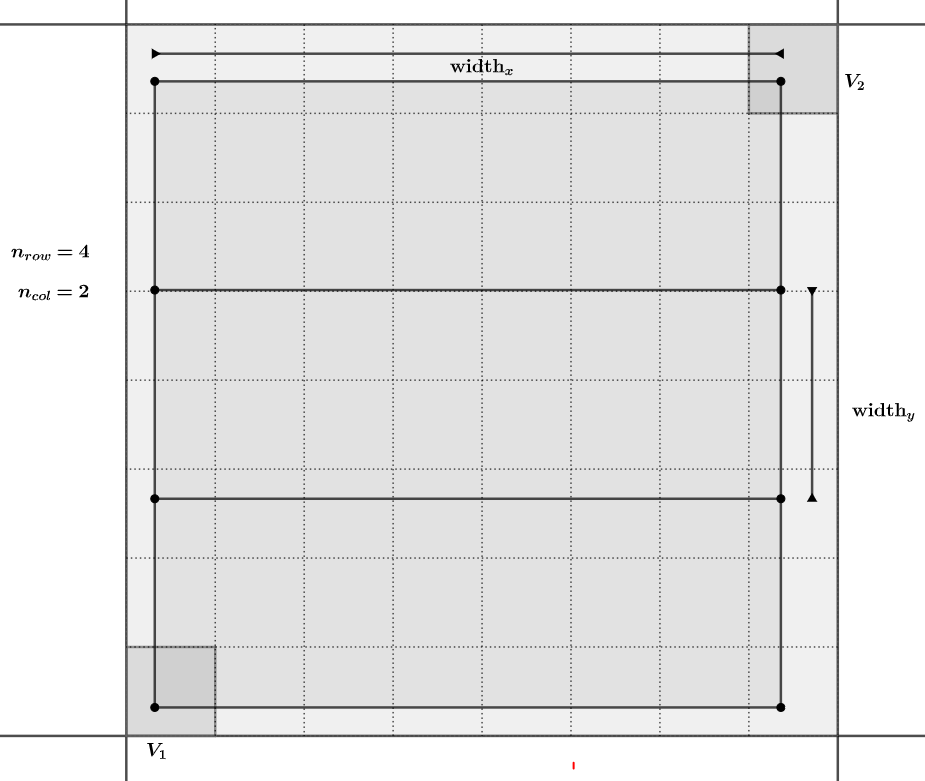
\includegraphics[width=1\linewidth]{Grid_generation.png}
% \end{center}
% \end{figure}


In this section we discuss the experimental results obtained testing the formulation presented in Section \ref{Form} and the matheuristic procedure proposed in Section \ref{Math} on a testbed of instances.\\
In particular, we consider instances of two typologies: the first one in which the targets to be visited are represented by points randomly located in a square of side 100 units, and the second one where the targets are represented by polygonals.\\
In this latter case, we set the cardinality of the set of points of the polygonal we want to build equal to 4 (this is for guaranteeing that the drone endurance is sufficient for traversing the whole polygonal) and we generate a random value $r$ in the interval $(5, 10)$. This value is used to generate a point $P=(P_x, P_y)$ inside the sub-square $[r, 100-r]^2$.\\
Next, sequentially, we generate a random angle $\alpha \in (0,2\pi)$ and from the current point $P$, we generate a new point $Q=(P_x+r*cos(\alpha), P_y + r*sin(\alpha))$. If point $Q$ belongs to the square $[r, 100-r]^2$, then we connect point $Q$ to point $P$ with a segment. Otherwise, we update $\alpha$ by adding $\pi/6$ to it until we obtain a point $Q^{'}=(P_x+r*cos(\alpha), P_y + r*sin(\alpha))$ that belongs to the square $[r, 100-r]^2$.
Then, the same procedure is repeated to generate the remaining break points of the polygonal.\\
For each of the two typologies, we generate instances of increasing size (number of targets) ranging between 5 and 15. For each size, we consider values of the drone endurance in the set $\{30,40,50,60,70\}$. For each combination of size and endurance value, we generate 5 instances.
We run the formulation on these instances by adopting two different commercial solvers, Cplex and Gurobi, setting a time limit of 2 hours.
Table \ref{table:tab1} shows the results of this comparison. Specifically, for each typology (Type 1 for points, Type 2 for polygonals), for each size and each endurance value, we report the number of instances for which the solvers are able to find at least a feasible solution of the problem within the time limit (\# f.i.), the average gap (Gap) and the average solution time in seconds (Time).





%\begin{figure}[h!]
%\begin{center}
% 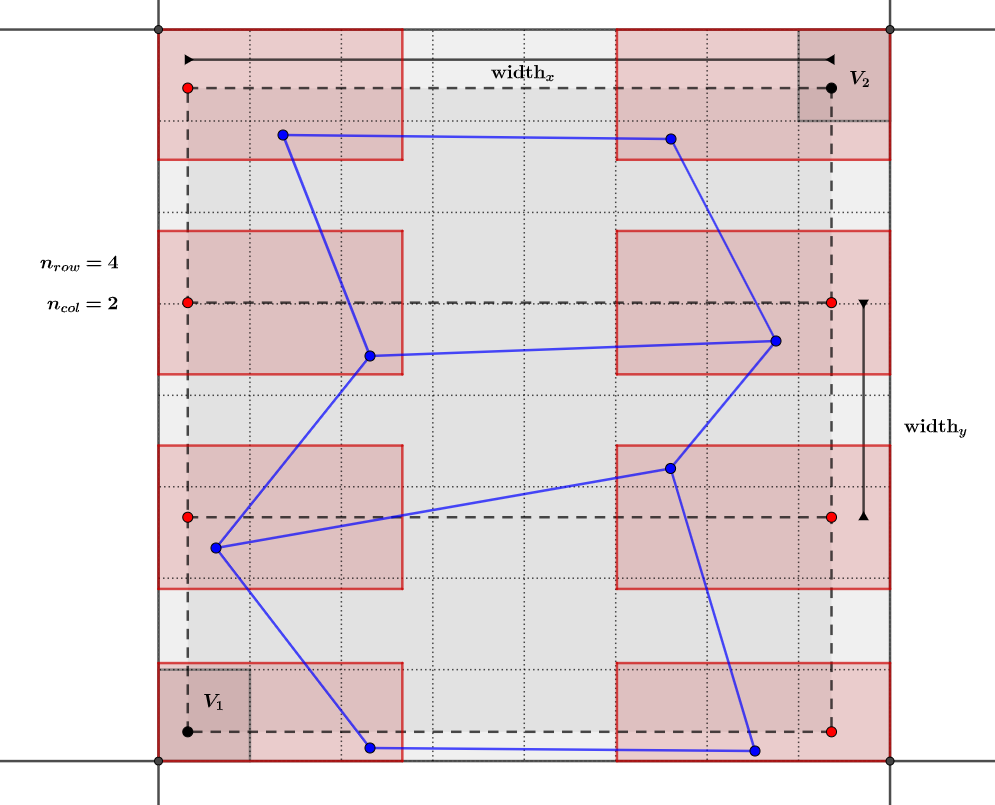
\includegraphics[width=0.6\linewidth]{Grid_generation_2.png}
%\end{center}
%\caption{Example of generation of a grid graph}
%\label{fig:fig1}
%\end{figure}
 
 


 
\begin{table}[!h]
\caption{Comparison between Cplex and Gurobi}
\centering
\tiny
\begin{tabular}{|c|c|c c c c c c|c c c c c c|}
\hline
\multirow{3}{*}{\textbf{|$\mathcal{T}$|}} & \multirow{3}{*}{\textbf{N}} & \multicolumn{6}{|c|}{\textbf{Type 1}} & \multicolumn{6}{|c|}{\textbf{Type 2}}\\
%\cline{4-15}
& & \multicolumn{3}{c|}{Cplex} & \multicolumn{3}{c|}{Gurobi} & \multicolumn{3}{c|}{Cplex} & \multicolumn{3}{c|}{Gurobi} \\
%\cline{3-15}
& & \# f.i. & Gap & Time & \# f.i. & Gap & Time & \# f.i. & Gap & Time & \# f.i. & Gap & Time\\
\hline
\multirow{5}{*}{\midrule 5} 
& 30 & 5 & 0 & 5,33 & 5 & 0 & 4.99 & 5 & 0 & 13,41 & 5 & 0 & 196.26\\
& 40 & 5 & 0 & 5,08 & 5 & 0 & 3.13 & 5 & 0 & 10,9 &  5 & 0 & 322.56\\
& 50 & 5 & 0 & 4,73 & 5 & 0 & 4.86 & 5 & 0 & 13,05 & 5 & 0 & 216.28\\
& 60 & 5 & 0 & 5,27 & 5 & 0 & 3.48 & 5 & 0 & 19,07 & 5 & 0 & 339.01\\
& 70 & 5 & 0 & 5,27 & 5 & 0 & 4.42 & 5 & 0 & 16,36 & 5 & 0 & 276.53\\
\hline
\multirow{5}{*}{\midrule 6} 
& 30 & 5 & 0 &  21,95 & 5 & 0 & 262.57 & 5 & 0 & 148.69 & 5 & 0.09 & 4250.68\\
& 40 & 5 & 0 &  30,5 & 5 & 0 & 106.7 &  5  & 0 & 238.77 &	5 &	0.14 &	5196.74\\
& 50 & 5 & 0 &	34,08 & 5 &	0 &	193.8 &  5 & 0 & 193.8  & 5 & 0.09 &	5333.45\\
& 60 & 5 & 0 &	33,39 &	5 &	0 &	138.46 & 5 & 0 & 185.92 & 4 & 0.25 &	6602.12\\
& 70 & 5 & 0 &	36,3 &	5 &	0 &	198.59 & 5 & 0 & 264.39 & 4 & 0.46 &	7200.52\\
\hline
\multirow{5}{*}{\midrule 7} 
& 30 &	5 &	0 &	229,75 & 5 & 0.11 &	4729.31 & 5 & 0    & 3063.24 & 2 &	0.62 &	7200.23\\
& 40 &	5 &	0 &	268,47 & 5 & 0.08 &	4060.19 & 5 & 0,06 & 3420.54 & 2 & 0.44 & 7200.11\\
& 50 &	5 &	0 &	255,35 & 5 & 0.23 &	6592.4  & 5 & 0,05 & 4034.04 & 3 &	0.58 &	7200.17\\
& 60 &	5 &	0 &	348,62 & 5 & 0.29 &	5879.46 & 5 & 0    & 4787.98 & 1 & 0.55 & 7200.17\\
& 70 &	5 &	0 &	301,47 & 5 & 0.27 &	6258.75 & 5 & 0    & 3986.24 & 0	& * & *\\
\hline
\multirow{5}{*}{\midrule 8} 
& 30 &	5 &	0 & 2265,56 & 5 & 0.73 & 7200.15 & 5 & 0,42 & 7200.02 & 1 &	0.73 &	7200.68\\
& 40 &	5 &	0 & 2820,11 & 5 & 0.61 & 7200.21 & 5 & 0,48 & 7200.02 & 0 & * & *\\
& 50 &	5 &	0 &	2877,69 & 5 & 0.65 & 7200.09 & 5 & 0,51 & 7200.02 & 0 & * & *\\
& 60 &	5 &	0 & 3159,62 & 5 & 0.76 & 7200.25 & 5 & 0,44 & 7200.02 &	0 &	* &	*\\
& 70 &	5 &	0 &	3188,16 & 5 & 0.72 & 7200.13 & 5 & 0,48 & 7200.02 &	0 &	* &	*\\
\hline
\multirow{5}{*}{\midrule 9} 
& 30 &  5 & 0,36 & 7200,03 & 5 & 0.86 &	7200.19 & 5 & 0,68 & 7200.03 &	0 &	* &	*\\
& 40 &	5 &	0,35 & 7200,02 & 5 & 0.89 &	7200.23 & 5 & 0,66 & 7200.02 & 0 & * & *\\
& 50 &	5 &	0,37 & 7200,1 & 5 & 0.83 &	7200.2  & 5 & 0,67 & 7200.02 & 0 & * & *\\
& 60 &	5 &	0,36 & 7200,1& 5 & 0.83  &	7200.18 & 5 & 0,66 & 7200.02 & 0 & * & *\\
& 70 &	5 &	0,33 & 7200,02 & 5 & 0.87 &	7200.24 & 5 & 0,64 & 7200.02 &	0 &	* & *\\
\hline
\multirow{5}{*}{\midrule 10} 
& 30 & 5 &	0,5 &	7200,42 & 5 & 0.92 & 7200.35 & 5 & 0,69 & 7200.03 &	0 &	* &	*\\
& 40 & 5 &	0,48 &	7200,62 & 5 & 0.91 & 7200.19 & 5 & 0,7 & 7200.04 &	0 &	* &	*\\
& 50 & 5 &	0,53 &	7200,47 & 5 & 0.92 & 7200.2  & 5 & 0,7 & 7200.04 & 0 & * & *\\
& 60 & 5 &	0,51 &	7200,94 & 5 & 0.92 & 7200.2  & 5 & 0,69 & 7200.14 & 0 & * & *\\
& 70 & 5 &	0,47 &	7201,19 & 5 & 0.92 & 7200.23 & 5 & 0,71 & 7200.04 &	0 &	* &	*\\
\hline
\multirow{5}{*}{\midrule 11} 
& 30 & 5 & 0,61 & 7200,35 &	5 &	0.94 & 7200.48 & 5 & 0,71 &	7200.03 & 0 & * & *\\
& 40 & 5 & 0,65 & 7200,2  &	5 &	0.95 & 7200.18 & 5 & 0,7 &	7200.07 & 0 & * & *\\
& 50 & 5 & 0,65 & 7200,42 &	5 &	0.93 & 7200.24 & 5 & 0,69 &	7200.03 & 0 & * & *\\
& 60 & 5 & 0,64 & 7200,54 &	5 &	0.94 & 7200.28 & 5 & 0,71 &	7200.04 & 0 & * & *\\
& 70 & 5 & 0,6 &  7201,07 &	5 &	0.93 & 7200.23 & 5 & 0,72 &	7200.03 & 0 & * & *\\
\hline
\multirow{5}{*}{\midrule 12} 
& 30 &	5 &	0,76 &	7200,59 &	5 &	 0.96 &	7200.24 &	5 &	0,72 &	7200.04 &	0 &	* &	*\\
& 40 &	5 &	0,75 &	7200,64 &	5 &	0.96 &	7200.29 &	5 &	0,72 &	7200.04 &	0 &	* &	*\\
& 50 &	5 &	0,72 &	7200,84 &	5 &	0.95 &	7200.28 &	5 &	0,72 &	7200.04 &	0 &	* &	*\\
& 60 &	5 &	0,74 &	7200,92 &	5 &	0.96 &	7200.22 &	5 &	0,71 &	7200.05 &	0 &	* &	*\\
& 70 &	5 &	0,71 &	7200,96 &	4 &	0.96 &	7200.25 &	5 &	0,71 &	7200.06 &	0 &	* &	*\\
\hline\multirow{5}{*}{\midrule 13} 
& 30 & 5 &0,85 & 7200,04 &	2 &	0.97 &	7200.31 &	5 &	0,76 &	7200.07 &	0 &	* &	*\\
& 40 & 5 &0,84 & 7200,06 &	2 &	0.96 &	7200.32 &	5 &	0,75 &	7200.04 &	0 &	* &	*\\
& 50 & 5 &0,82 & 7200,13 &	1 &	0.96 &	7200.24 &	5 &	0,75 &	7200.04 &	0 &	* &	*\\
& 60 & 5 &0,82 & 7200,08 &	2 &	0.97 &	7200.32 &	5 &	0,74 &	7200.05 &	0 &	* &	*\\
& 70 & 5 &0,83 & 7200,3  &	3 &	0.97 &	7200.4  &	5 &	0,75 &	7200.06 &	0 &	* &	*\\
\hline\multirow{5}{*}{\midrule 14} 
& 30 &	5 &	0,91 &	7200,26 &	0 &	* &	* &	5 &	0,73 &	7200.06 &	0 &	* &	*\\
& 40 &	5 &	0,9  &	7200,04 &	0 &	* &	* &	5 &	0,72 &	7200.07 &	0 &	* & *\\
& 50 &	5 &	0,89 &	7200,28 &	0 &	* &	* &	5 &	0,72 &	7200.06 &	0 &	* &	*\\
& 60 &	5 &	0,89 &	7200,23 &	0 &	* &	* &	5 &	0,73 &	7200.08 &	0 &	* &	*\\
& 70 &	5 &	0,91 &	7200,22 &	0 &	* &	* &	5 &	0,71 &	7200.05 &	0 &	* &	*\\
\hline
\multirow{5}{*}{\midrule 15} 
& 30 &	5 &	0,92 &	7200,07 &	0 &	* &	* &	5 &	0,72 &	7200.12 &	0 &	* &	*\\
& 40 &	5 &	0,9  &	7200,05 &	0 &	* &	* &	5 &	0,7 &	7200.08 &	0 &	* &	*\\
& 50 &	5 &	0,91 &	7200,25 &	0 &	* &	* &	5 &	0,72 &	7200.19 &	0 &	* &	*\\
& 60 &	5 &	0,92 &	7200,19 &	0 &	* &	* &	5 &	0,73 &	7200.41 &	0 &	* &	*\\
& 70 &	5 &	0,93 &	7200,22 &	0 &	* &	* &	5 &	0,71 &	7200.08 &	0 &	* &	*\\
\hline
\end{tabular}
\label{table:tab1}
\end{table}


\noindent


From Table \ref{table:tab1} we can observe that there is a significant difference in the solvers performances. Indeed, Gurobi is not able to find a feasible solution, within the time limit,  for any of  the instances of Type 1 for the largest size instances ($|\mathcal{T}|\in \{14,15\}$)  and for instances of Type 2 from size 8 and drone endurance equal to 40. Moreover, for instances of Type 1 and sizes 12 and 13 and for instances of Type 2 and sizes 6, 7 and 8, it is able to find a feasible solution only for a subset of them, as reported by the counter $\#$ f.i.\\
On the contrary, Cplex is always able to find  feasible solutions for all instances of both Types and for all sizes.\\
\indent This behaviour of the two solvers seems to be explainable by the different internal implementation for handling the lazy constraints in the formulations during the solution process. Indeed, by analyzing the .mps files generated by both solvers, we found out that Gurobi embeds the lazy constraints directly before to start  the branch and bound procedure, while Cplex adds them during the solution procedure when they are actually needed. This difference leads Gurobi to load and solve a more complex formulation since the beginning of the solution procedure. For this reason it is not able to find a feasible solution in 2 hours for most of the largest instances.\\
\indent Regarding the number of instances solved to optimality, Cplex can solve instances up to size 8 of Type 1 within the time limit. In particular, it is able to solve, in average, in less than 6 seconds instances of size 5, in at most 36 seconds instances of size 6, in less than 6 minutes instances of size 7 and in at most 53 minutes instances of size 8. We can observe that the average solution time, increases by an order of magnitude, with respect to the instance size,  up to size 8 and for larger size instances it reaches the time limit of 2 hours. Also considering the comparison between Cplex and Gurobi, we can observe a difference of an order of magnitude in the solution times for Type 1 instances up to size 7 and for Type 2 instances up to size 6.\\
The average gap associated with the solutions provided by both Cplex and Gurobi, ranges between 0.05 and 0.93 and it increases with the instances size. The instances of Type 2 seem to be the most difficult to solve. Indeed, depending on the instances size, the solution time is one or two orders of magnitude greater than that for instances of Type 1. However, from instances of size 12, we can observe that the average gap associated with instances of Type 1, solved by means of Cplex, is always greater than the one associated with instances of Type 2.





\begin{table}[!h]
\caption{Exact solution via Cplex with and without initialization}
\centering
\tiny
\begin{tabular}{|c|c|c c c c|c c c c|}
\hline
\multirow{2}{*}{\textbf{|$\mathcal{T}$|}} & \multirow{2}{*}{\textbf{N}} & \multicolumn{4}{|c|}{\textbf{Type 1}} & \multicolumn{4}{|c|}{\textbf{Type 2}}\\
& &  Gap (i) & Time\_h  & Time\_f & Gap (wi) &  Gap (i) & Time\_h  & Time\_f & Gap (wi)\\
\hline
\multirow{5}{*}{\midrule 5} 
& 30 &	0 &	0,29 &	4,04 &	0 &	0 &	1.42 &	16.83 &	0\\
& 40 &	0 &	0,21 &	3,88 &	0 &	0 &	1.47 &	17.17 &	0\\ 
& 50 &	0 &	0,25 &	4,05 &	0 &	0 &	1.45 &	20.31 &	0\\
& 60 &	0 &	0,32 &	4,72 &	0 &	0 &	1.42 &	20.75 &	0\\
& 70 &	0 &	0,25 &	4,13 &	0 &	0 &	1.46 &	25.54 &	0\\
\hline
\multirow{5}{*}{\midrule 6} 
& 30 &	0 &	0,2 &	18,66 &	0 &	0 &	2.41 &	286.12 &	0\\
& 40 &	0 &	0,17 &	17,92 &	0 &	0 &	2.55 &	394.29 &	0\\
& 50 &	0 &	0,12 &	19,35 &	0 &	0 &	2.35 &	383.94 &	0\\
& 60 &	0 &	0,16 &	19,72 &	0 &	0 &	2.24 &	322.92 &	0\\
& 70 &	0 &	0,18 &	23,35 &	0 &	0 &	2.69 &	413.62 &	0\\
\hline
\multirow{5}{*}{\midrule 7} 
& 30 &	0 &	0,21 &	201,92 &	0 &	0 &	4.25 &	2806.77 &	0\\
& 40 &	0 &	0,46 &	204,39 &	0 &	0.03 &	4.07 &	4651.65 &	0.06\\
& 50 &	0 &	0,35 &	213,41 &	0 &	0.15 &	3.87 &	5409.26 &	0.05\\
& 60 &	0 &	0,46 &	208,24 &	0 &	0.12 &	4.58 &	6281.02 &	0\\
& 70 &	0 &	0,39 &	243,37 &	0 &	0.06 &	4.48 &	6103.81 &	0\\
\hline
\multirow{5}{*}{\midrule 8} 
& 30 &	0 &	0,7 &	1619,37 &	0 &	0.5  &	7.61 &	7200.03 &	0.42\\
& 40 &	0 &	0,47 &	2333,97 &	0 &	0.52 &	7.65 &	7200.03 &	0.48\\
& 50 &	0 &	0,48 &	2020,92 &	0 &	0.5  &	7.45 &	7200.03 &	0.51\\
& 60 &	0 &	0,63 &	2484,49 &	0 &	0.47 &	7.02 &	7200.15 &	0.44\\
& 70 &	0 &	0,62 &	2724,14 &	0 &	0.49 &	7.8 &	7200.09 &	0.48\\
\hline
\multirow{5}{*}{\midrule 9} 
& 30 &	0,27 &	0,94 &	7200,15 &	0,36 &	0.65 &	13.64 &	7200.06 &	0.68\\
& 40 &	0,33 &	0,91  &	7200,71 &	0,35 &	0.66 &	12.31 &	7200.03 &	0.66\\
& 50 &	0,29 &	0,9  &	7200,37 &	0,37 &	0.66 &	14.88 &	7200.04 &	0.67\\
& 60 &	0,36 &	0,72  &	7200,4 &	0,36 &	0.66 &	14.63 &	7200.03 &	0.66\\
& 70 &	0,31 &	0,68  &	7200,55 &	0,33 &	0.63 &	13.37 &	7200.03 &	0.64\\
\hline
\multirow{5}{*}{\midrule 10} 
& 30 &	0,45 &	1,43 &	7200,99 &	0,5  &	0.66 &	22.58 &	7200.02 &	0.69\\
& 40 &	0,48 &	1,68 &	7201,77 &	0,48 &	0.64 &	20.89 &	7200.02 &	0.7\\
& 50 &	0,44 &	1,61 &	7201,67 &	0,53 &	0.68 &	21.31 &	7200.16 &	0.7\\
& 60 &	0,49 &	1,74&	7201,77 &	0,51 &	0.66 &	22.1 &	7200.03 &	0.69\\
& 70 &	0,46 &	1,8 &	7201,99 &	0,47 &	0.67 &	23.62 &	7200.03 &	0.71\\
\hline
\multirow{5}{*}{\midrule 11} 
& 30 &	0,54 &	1,8 &	7201,87 &	0,61 &	0.67 &	34.72 &	7200.03 &	0.71\\
& 40 &	0,55 &	2,1 &	7201,78 &	0,65 &	0.67 &	34.9 &	7200.12 &	0.7\\
& 50 &	0,54 &	2,12 &	7201,68&	0,65 &	0.68 &	34.31 &	7200.13 &	0.69\\
& 60 &	0,58 &	2    &	7201,54 &	0,64 &	0.68 &	34.9 &	7200.07 &	0.71\\
& 70 &	0,56 &	2,11 &	7201,75 &	0,6 &	0.68 &	35.02 &	7200.03 &	0.72\\
\hline
\multirow{5}{*}{\midrule 12} 
& 30 &	0,66 &	3,14 &	7201,16 &	0,76 &	0.68 &	51.52 &	7200.18 &	0.72\\
& 40 &	0,67 &	3,43 &	7201,26 &	0,75 &	0.68 &	53.85 &	7200.15 &	0.72\\
& 50 &	0,74 &	3,04 &	7201,15 &	0,72 &	0.69 &	53.02 &	7200.08 &	0.72\\
& 60 &	0,72 &	2,97 &	7201,35 &	0,74 &	0.68 &	53.83 &	7200.07 &	0.71\\
& 70 &	0,71 &	3,12 &	7201,67 &	0,71 &	0.68 &	58.29 &	7200.04 &	0.71\\

\hline\multirow{5}{*}{\midrule 13} 
& 30 &  0,81  &	5,42 &	7200,86 &	0,85 &  0.72  &	78.7  &	7200.1  &	0.76\\
& 40 &	0,8   &	4,3 &	7201,14 &	0,84 &  0.72  &	83.12 &	7200.03 &	0.75\\
& 50 &	0,83  &	5,46 &	7201,09 &	0,82 &	0.72 &	79.63 &	7200.08 &	0.75\\
& 60 &	0,81  &	4,16 &	7201,16 &	0,82 &	0.72 &	86.79 &	7200.08 &	0.74\\
& 70 &	0,82  &	4,28 &	7201,1 &	0,83 &	0.72 &	83.36 &	7200.04 &	0.75\\

\hline\multirow{5}{*}{\midrule 14} 
& 30 &  0,85  &	6,75 &	7201,03 &	0,91 &	0.67 &	107.31 &	7200.16 &	0.73\\
& 40 &	0,84 &	5,88 &	7201,02 &	0,9  &  0.67 &	110.38 &	7200.04 &	0.72\\
& 50 &	0,87 &	6,07 &	7201,29 &	0,89 &	0.67 &	107.14 &	7200.15 &	0.72\\
& 60 &	0,85 &	5,71 &	7201,15 &	0,89 &	0.67 &	112.05 &	7200.04 &	0.73\\
& 70 &	0,84 &	6,4 &	7200,97 &	0,91 &	0.67 &	111.62 &	7200.06 &	0.71\\
\hline
\multirow{5}{*}{\midrule 15} 
& 30 &	0,87 &	7,1 &	7202,06 & 0,92 &	0.64 &	141.05 &	7200.27 &	0.72\\
& 40 &	0,87 &	7   &	7201,2  & 0,9  &	0.64 &	146.34 &	7200.27 &	0.7\\
& 50 &	0,88 &	9,47 &	7200,87 & 0,91 &	0.63 &	132.54 &	7200.26 &	0.72\\
& 60 &	0,88 &	6,31 &	7201,39 & 0,92 &	0.63 &	144.69 &	7200.27 &	0.73\\
& 70 &	0,88 &	7,15 &	7201,33 & 0,93 &	0.64 &	140.05 &	7200.21 &	0.71\\
\hline
\end{tabular}
\label{table:tab2}
\end{table}
%}


Table \ref{table:tab2} summarizes the comparison between the exact solution of the formulation via Cplex, with and without initialization with the solution found by the matheuristic algorithm. For each typology of instances and for each size and drone endurance, we report the average gap with initialization (Gap (i)), the average running time of the matheuristic (Time\_h), the average running time of the formulation (Time\_f) and the average gap without initialization (Gap (wi)). We can observe that the matheuristic  provides a solution of the problem in less than 1 second for instances of Type 1 up to 9 targets and in less than 10 seconds for instances of Type 1 up to 15 targets. The polygonals instances (Type 2) are more challenging to be solved with solution times of the matheuristic ranging between 1.42 seconds and 2.4 minutes. However, comparing these times with those required by exact solution of the formulation, we can conclude that the matheuristic algorithm is a very good alternative to the exact solver. Moreover, we can observe that when the solution provided by the matheuristic algorithm is used to initialize the solver for the formulation, in most of the cases the final average gap slightly decreases after the time limit is reached. The most significant reduction in the average gap can be observed for the largest size instances of Type 2 for which the average gap with initialization is up to 13$\%$ lower than the one without initialization. As regards the computation times for the exact solution method, we can also observe that if the solution provided by the matheuristic algorithm is used to initialize the solver, the convergence to the optimal solution for instances of Type 1 up to 8 targets is significantly improved.




\begin{table}[!h]
\caption{Exact solution via Gurobi with and without initialization}
\centering
\tiny
\begin{tabular}{|c|c|c c c c|c c c c|}
\hline
\multirow{2}{*}{\textbf{|$\mathcal{T}$|}} & \multirow{2}{*}{\textbf{N}} & \multicolumn{4}{|c|}{\textbf{Type 1}} & \multicolumn{4}{|c|}{\textbf{Type 2}}\\
& & Gap (i) & Time\_h  & Time\_f & Gap (wi) & Gap (i) & Time\_h  & Time\_f & Gap (wi)\\
\hline
\multirow{5}{*}{\midrule 5} & 30 & 0 &	0.01 &	2.15 &	0 &	0 &	0.37 &	71.63 &	0\\
%\cline{4-15}
& 40 & 0 &	0.01 &	1.94 &	0 &	0 &	0.34 &	63.95 &	0\\
%\cline{4-15}
& 50 & 0 &	0.01 &	2.11 &	0 &	0 &	0.35 &	75.82 &	0\\
%\cline{4-15}
& 60 & 0 &	0.01 &	1.59 &	0 &	0 &	0.35 &	103.98 &	0\\
%\cline{4-15}
& 70 & 0 &	0.01 &	1.76 &	0 &	0 &	0.35 &	141.09 &	0\\
\hline
\multirow{5}{*}{\midrule 6} & 30 & 0 &	0.01 &	33.6 &	0 &	0 &	0.64 &	642.4 &	0.09\\
& 40 & 0 &	0.01 &	29.34 &	0 &	0 &	0.69 &	1131.4 &	0.14\\
& 50 &	0 &	0.01 &	66.03 &	0 &	0 &	0.68 & 	1362 &	0.09\\
& 60 &	0 &	0.01 &	73.52 &	0 &	0 &	0.68 &	2161.66 &	0.25\\
& 70 &	0 &	0.01 &	49.35 &	0 &	0 &	0.73 &	2011.79 &	0.46\\
\hline
\multirow{5}{*}{\midrule 7} & 30 & 0 &	0.02 &	1113.79	& 0.11 &	0.29 &	1.07 &	6680.17 &	0.62\\
& 40 &	0 &	0.02 &	585.02	& 0.08 &	0.36 &	1.01 &	6969.07 &	0.44\\
& 50 & 0 &	0.02 &	1193.87 &	0.23 &	0.35 &	1.04 &	6708.26 &	0.58\\
& 60 &	0 &	0.02 &	1474.48 &	0.29 &	0.32 &	1.09 &	6871.41 &	0.55\\
& 70 &	0 &	0.02 &	1046.2 &	0.27 &	0.42 &	1.06 &	7200.19 &	*\\
\hline
\multirow{5}{*}{\midrule 8} & 30 &	0.09 &	0.02 &	4446.46 &	0.73 &	0.63 &	3.03 &	7200.19 &	0.73\\
& 40 &	0.18 &	0.02 &	5660.75 &	0.61 &	0.62 &	1.34 &	7200.16 &	*\\
& 50 &	0.28 &	0.02 &	6581.53 &	0.65 &	0.62 &	1.36 &	7200.19 &	*\\
& 60 &	0.32 &	0.02 &	6112.57	& 0.76 &	0.63 &	1.45 &	7200.25 &	*\\
& 70 &	0.21 &	0.02 &	5863.52 &	0.72 &	0.62 &	1.42 &	7200.14 &	*\\
\hline
\multirow{5}{*}{\midrule 9} & 30 & 0.55 &	0.04 &	7200.16 &	0.86 &	0.72 &	3.28 &	7200.14	 & *\\
& 40 &	0.49 &	0.04 &	7200.15 &	0.89 &	0.71 &	3.24 &	7200.12	& *\\
& 50 &	0.61 &	0.03 &	7200.12	& 0.83	& 0.7 &	3.16 &	7200.13 &	*\\
& 60 &	0.55 &	0.03 &	7200.16 &	0.83 &	0.7 &	3.27 &	7200.11 &	*\\
& 70 & 0.44 &	0.03 &	7200.21 &	0.87 &	0.71 &	3.26 &	7200.11	& *\\
\hline
\multirow{5}{*}{\midrule 10} & 30 &	0.66 &	0.06 &	7200.23 &	0.92 &	0.7 &	8.27 &	7200.15 &	*\\
& 40 &	0.65 &	0.06 &	7200.21 &	0.91 &	0.69 &	8.19 &	7200.17 &	*\\
& 50 &	0.64 &	0.05 &	7200.19	 & 0.92 &	0.69 &	8.21 &	7200.15 &	*\\
& 60 &	0.62 &	0.06 &	7200.22 &	0.92 &	0.68 &	8.13 &	7200.15 &	*\\
& 70 &	0.68 &	0.07 &	7200.18 &	0.92 &	0.7 &	8.3 &	7200.13	& *\\
\hline
\multirow{5}{*}{\midrule 11} & 30 &	0.7	& 0.11 &	7200.37	& 0.94	& 0.68 &	11.7 &	7200.2 & *\\
& 40 &	0.73 &	0.11 &	7200.2	& 0.95 &	0.68 &	11.71 &	7200.1 &	*\\
& 50 &	0.69 &	0.11 &	7200.21 &	0.93 &	0.67 &	11.71 &	7200.15 &	*\\
& 60 &	0.71 &	0.11 &	7200.21	 & 0.94 &	0.67 &	11.65 &	7200.16 &	*\\
& 70 &	0.72 &	0.11 &	7200.2 &	0.93 &	0.67 &	11.68 &	7200.14	& *\\
\hline
\multirow{5}{*}{\midrule 12} & 30 &	0.83 &	0.25 &	7200.22 &	0.96 &	0.68 &	15.83 &	7200.09 &	*\\
& 40 &	0.83 &	0.25 &	7200.27 &	0.96 &	0.68 &	15.76 &	7200.14 &	*\\
& 50 &	0.85 &	0.26 &	7200.19	& 0.95	& 0.68 &	23.28 &	7201.3 &	*\\
& 60 &	0.84 &	0.25 &	7200.28 &	0.96 &	0.68 &	15.92 &	7201.16 &	*\\
& 70 &	0.87 &	0.31 &	7200.22 &	0.96 &	0.69 &	15.85 &	7201.7 &	*\\
\hline\multirow{5}{*}{\midrule 13} & 30 &	0.92 &	0.8	& 7200.29 &	0.97 &	0.71 &	26.34 &	7200.23	& *\\
& 40 &	0.89 &	0.85 &	7200.5	& 0.96 &	0.71 &	26.41 &	7200.24 &	*\\
& 50 &	0.91 &	0.82 &	7200.72 &	0.96 &	0.71 &	26.41 &	7200.4	 &*\\
& 60 &	0.89 &	0.8 &	7200.37 &	0.97 &	0.71 &	26.43 &	7200.26 &	*\\
& 70 &	0.92 &	0.84 &	7200.41 &	0.97 &	0.71 &	26.33 &	7200.22 &	*\\
\hline\multirow{5}{*}{\midrule 14} & 30 &	0.95 &	2.95 &	7200.7 &	* &	0.67 &	52.07 &	7280.27 &	*\\
& 40 &	0.95 &	2.87 &	7200.81 &	* &	0.67 &	61.06 &	7200.33 &	*\\
& 50 &	0.95 &	2.87 &	7200.77 &	* &	0.67 &	78.34 &	7200.34 &	*\\
& 60 &	0.96 &	2.91 &	7200.87 &	* &	0.67 &	61.55 &	7200.28 &	*\\
& 70 &	0.93 &	2.92 &	7201.08 &	* &	0.67 &	52.78 &	7200.37 &	*\\
\hline
\multirow{5}{*}{\midrule 15} & 30 &	0.99 &	8.71 &	7200.4 &	* &	0.62 &	99.44 &	7200.55	& *\\
& 40 &	1 &	8.54 &	7200.61	& *	 & 0.62	& 84.45	& 7200.54 &	*\\
& 50 &	1 &	8.43 &	7200.36	& *	& 0.62 &	124.48 &	7201.41 &	*\\
& 60 &	1 &	8.35 &	7200.5 &	* &	0.63 &	139.61	& 7200.8 &	*\\
& 70 &	1 &	8.48 &	7200.27 &	* &	0.63 &	109.46 &	7200.33 &	*\\
\hline
\end{tabular}
\label{table:tab3}
\end{table}


Similarly, Table \ref{table:tab3} reports the comparison between the exact solution of the formulation via Gurobi, with and without initialization with the solution found by the matheuristic algorithm. In this case, the initialization permits to overcome the problem met by the Gurobi solver that, as also reported in Table \ref{table:tab1}, was not able to find a feasible solution for instances of Type 1 from size 14 and for instances of Type 2 from size 8. In particular, we can observe that for instances of Type 1 and from size 9, the initialization with the matheuristic solution improves more than with respect to same process in Cplex in terms of average gap.


In Figure \ref{fig:Fig4} and Figure \ref{fig:Fig5} we show the boxplots representing the gap values for the different instance sizes, distinguishing between the two typologies (Type 1: point or Type 2: polygonal targets) respectively by using Gurobi and Cplex. On the left of both figures we can observe the gap values obtained by solving the formulation without initialization, while on the right, the ones obtained by providing to the solvers the initial solution generated by the matheuristic algorithm. 
Specifically, we can visualize that the gap values for instances with point targets (Type 1) increase with the problem size in the exact solution both without and with initialization and with both solvers. However, as already observed in Table \ref{table:tab1}, Gurobi solver without initialization is not able to solve point instances of size 14 and 15. As regards the polygonal instances (Type 2), we can observe a different behaviour with respect to the gap, which increases with the instances size up to 9 targets. From instances of size 10 its gap, excluding outliers, always ranges in the interval [0.6, 0.8]. This can be still observed also by initializing the exact solution of the formulation even if, as already mentioned, in this latter case the gap values decrease and in most of the cases they belong to the interval [0.6,0.7], always excluding outliers. Thus, the polygonal instances are more difficult than the point instances for sizes up to 10. For bigger size instances, the gap value for polygonal instances consistently belongs to a fixed interval, while the gap for point instances increases with the size. 

In order to further investigate this behaviour, we run the mathematical programming formulation with Cplex on one of the biggest size instances with 15 targets and endurance equal to 40, for both types of targets (Type 1 and 2) and setting a time limit of 24 hours. Figure \ref{fig:Fig6} reports the objective function value and the lower bound value obtained over time, respectively, for the point and the polygonal targets versions of this instance. We can observe that the initial value of the lower bound for the point targets instance is equal to 0 while the one for the polygonal targets instance is equal to 331. This difference is due to the different structure of the targets. Indeed, for the polygonal targets the formulation includes the constraint imposing the visit of a given minimum percentage of each polygonal. This implies that the first value of the lower bound is greater than 0. Thus, while the solution process for the point targets instance starts from a gap equal to 100\%, the one for the polygonal targets instance starts from a gap equal to 80\%, as we can also observe in Figure \ref{fig:Fig6}. This different initial gap allows the solver to slowly improve it in the first case but not in the second one. Actually, only after around 15 hours of cpu, we can observe that the two gaps (for the instance of Type 1 and 2) are equal and then the value of the gap for the point targets instance continues to decrease, whereas the one related to the polygonal targets instance does not change in the remaining time. This is explained because the lower bound of the point targets instance improves over time, see Figure \ref{fig:Fig6}, but it does not change at all for the polygonal targets instance.
This behaviour shows that the instances of Type 2 (polygonal targets) are still more difficult to be solved than the instances of Type 1 (point targets). However, the different structure of the targets provides an initial advantage in the lower bound of the polygonal target instances, due to the constraint related to the minimum percentage of each polygonal to be visited, that can be exploited by the solver for the biggest sizes.




% \DeclareUnicodeCharacter{2212}{−}
% \usepgfplotslibrary{groupplots}
\usetikzlibrary{patterns,shapes.arrows}
\pgfplotsset{compat=newest}

\begin{figure}
    \centering
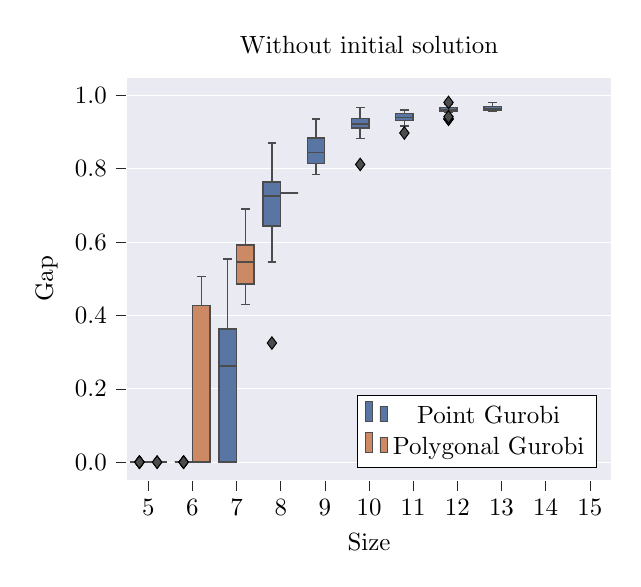
\begin{tikzpicture}[scale=0.9]

\definecolor{color0}{rgb}{0.917647058823529,0.917647058823529,0.949019607843137}
\definecolor{color1}{rgb}{0.347058823529412,0.458823529411765,0.641176470588235}
\definecolor{color2}{rgb}{0.798529411764706,0.536764705882353,0.389705882352941}

\begin{axis}[
axis background/.style={fill=color0},
axis line style={white},
tick align=outside,
title={Without initial solution},
x grid style={white},
xtick pos = left,
ytick pos = left,
xlabel={Size},
% xmajorticks=false,
xmin=-0.5, xmax=10.5,
xtick style={color=white!15!black},
xtick={0,1,2,3,4,5,6,7,8,9,10},
xticklabels={5,6,7,8,9,10,11,12,13,14,15},
y grid style={white},
ylabel={Gap},
ymajorgrids,
% ymajorticks=false,
ymin=-0.05, ymax=1.05,
ytick style={color=white!15!black},
ytick={-0.2,0,0.2,0.4,0.6,0.8,1,1.2},
yticklabels={−0.2,0.0,0.2,0.4,0.6,0.8,1.0,1.2},
legend pos = south east
]
\path [draw=white!29.8039215686275!black, fill=color1, semithick]
(axis cs:-0.396,0)
--(axis cs:-0.004,0)
--(axis cs:-0.004,8.98248411138978e-07)
--(axis cs:-0.396,8.98248411138978e-07)
--(axis cs:-0.396,0)
--cycle;
\path [draw=white!29.8039215686275!black, fill=color2, semithick]
(axis cs:0.004,0)
--(axis cs:0.396,0)
--(axis cs:0.396,9.66489035941329e-08)
--(axis cs:0.004,9.66489035941329e-08)
--(axis cs:0.004,0)
--cycle;
\path [draw=white!29.8039215686275!black, fill=color1, semithick]
(axis cs:0.604,8.98986405268812e-10)
--(axis cs:0.996,8.98986405268812e-10)
--(axis cs:0.996,5.60540837060592e-08)
--(axis cs:0.604,5.60540837060592e-08)
--(axis cs:0.604,8.98986405268812e-10)
--cycle;
\path [draw=white!29.8039215686275!black, fill=color2, semithick]
(axis cs:1.004,0)
--(axis cs:1.396,0)
--(axis cs:1.396,0.427084438776731)
--(axis cs:1.004,0.427084438776731)
--(axis cs:1.004,0)
--cycle;
\path [draw=white!29.8039215686275!black, fill=color1, semithick]
(axis cs:1.604,4.49224810355924e-08)
--(axis cs:1.996,4.49224810355924e-08)
--(axis cs:1.996,0.3635628352316)
--(axis cs:1.604,0.3635628352316)
--(axis cs:1.604,4.49224810355924e-08)
--cycle;
\path [draw=white!29.8039215686275!black, fill=color2, semithick]
(axis cs:2.004,0.485064480157975)
--(axis cs:2.396,0.485064480157975)
--(axis cs:2.396,0.59178368299242)
--(axis cs:2.004,0.59178368299242)
--(axis cs:2.004,0.485064480157975)
--cycle;
\path [draw=white!29.8039215686275!black, fill=color1, semithick]
(axis cs:2.604,0.64367384405556)
--(axis cs:2.996,0.64367384405556)
--(axis cs:2.996,0.763509282158919)
--(axis cs:2.604,0.763509282158919)
--(axis cs:2.604,0.64367384405556)
--cycle;
\path [draw=white!29.8039215686275!black, fill=color2, semithick]
(axis cs:3.004,0.733231325585761)
--(axis cs:3.396,0.733231325585761)
--(axis cs:3.396,0.733231325585761)
--(axis cs:3.004,0.733231325585761)
--(axis cs:3.004,0.733231325585761)
--cycle;
\path [draw=white!29.8039215686275!black, fill=color1, semithick]
(axis cs:3.604,0.814772123183105)
--(axis cs:3.996,0.814772123183105)
--(axis cs:3.996,0.883787998313117)
--(axis cs:3.604,0.883787998313117)
--(axis cs:3.604,0.814772123183105)
--cycle;
\path [draw=white!29.8039215686275!black, fill=color1, semithick]
(axis cs:4.604,0.911082622376599)
--(axis cs:4.996,0.911082622376599)
--(axis cs:4.996,0.937129107128515)
--(axis cs:4.604,0.937129107128515)
--(axis cs:4.604,0.911082622376599)
--cycle;
\path [draw=white!29.8039215686275!black, fill=color1, semithick]
(axis cs:5.604,0.931197050840517)
--(axis cs:5.996,0.931197050840517)
--(axis cs:5.996,0.95069453328678)
--(axis cs:5.604,0.95069453328678)
--(axis cs:5.604,0.931197050840517)
--cycle;
\path [draw=white!29.8039215686275!black, fill=color1, semithick]
(axis cs:6.604,0.957223620144976)
--(axis cs:6.996,0.957223620144976)
--(axis cs:6.996,0.966526130549437)
--(axis cs:6.604,0.966526130549437)
--(axis cs:6.604,0.957223620144976)
--cycle;
\path [draw=white!29.8039215686275!black, fill=color1, semithick]
(axis cs:7.604,0.960535638441675)
--(axis cs:7.996,0.960535638441675)
--(axis cs:7.996,0.969719696205704)
--(axis cs:7.604,0.969719696205704)
--(axis cs:7.604,0.960535638441675)
--cycle;
\draw[draw=white!29.8039215686275!black,fill=color1,line width=0.3pt] (axis cs:0,0) rectangle (axis cs:0,0);
\addlegendimage{ybar,ybar legend,draw=white!29.8039215686275!black,fill=color1,line width=0.3pt}
\addlegendentry{Point Gurobi}

\draw[draw=white!29.8039215686275!black,fill=color2,line width=0.3pt] (axis cs:0,0) rectangle (axis cs:0,0);
\addlegendimage{ybar,ybar legend,draw=white!29.8039215686275!black,fill=color2,line width=0.3pt}
\addlegendentry{Polygonal Gurobi}

\addplot [semithick, white!29.8039215686275!black]
table {%
-0.2 0
-0.2 0
};
\addplot [semithick, white!29.8039215686275!black]
table {%
-0.2 8.98248411138978e-07
-0.2 1.07793137211359e-06
};
\addplot [semithick, white!29.8039215686275!black]
table {%
-0.298 0
-0.102 0
};
\addplot [semithick, white!29.8039215686275!black]
table {%
-0.298 1.07793137211359e-06
-0.102 1.07793137211359e-06
};
\addplot [black, mark=diamond*, mark size=2.5, mark options={solid,fill=white!29.8039215686275!black}, only marks]
table {%
-0.2 1.29824871749342e-05
-0.2 5.09137094986383e-05
-0.2 4.65970322673504e-05
-0.2 8.38822928219561e-06
-0.2 2.18754724738788e-05
};
\addplot [semithick, white!29.8039215686275!black]
table {%
0.2 0
0.2 0
};
\addplot [semithick, white!29.8039215686275!black]
table {%
0.2 9.66489035941329e-08
0.2 2.11239141921176e-07
};
\addplot [semithick, white!29.8039215686275!black]
table {%
0.102 0
0.298 0
};
\addplot [semithick, white!29.8039215686275!black]
table {%
0.102 2.11239141921176e-07
0.298 2.11239141921176e-07
};
\addplot [black, mark=diamond*, mark size=2.5, mark options={solid,fill=white!29.8039215686275!black}, only marks]
table {%
0.2 6.98066581965961e-07
0.2 7.98566710418127e-07
};
\addplot [semithick, white!29.8039215686275!black]
table {%
0.8 8.98986405268812e-10
0.8 0
};
\addplot [semithick, white!29.8039215686275!black]
table {%
0.8 5.60540837060592e-08
0.8 1.28548312443731e-07
};
\addplot [semithick, white!29.8039215686275!black]
table {%
0.702 0
0.898 0
};
\addplot [semithick, white!29.8039215686275!black]
table {%
0.702 1.28548312443731e-07
0.898 1.28548312443731e-07
};
\addplot [black, mark=diamond*, mark size=2.5, mark options={solid,fill=white!29.8039215686275!black}, only marks]
table {%
0.8 1.84994910379735e-07
0.8 1.76228584193879e-06
0.8 1.89089629637651e-07
0.8 1.6573579259642e-05
};
\addplot [semithick, white!29.8039215686275!black]
table {%
1.2 0
1.2 0
};
\addplot [semithick, white!29.8039215686275!black]
table {%
1.2 0.427084438776731
1.2 0.506584603717493
};
\addplot [semithick, white!29.8039215686275!black]
table {%
1.102 0
1.298 0
};
\addplot [semithick, white!29.8039215686275!black]
table {%
1.102 0.506584603717493
1.298 0.506584603717493
};
\addplot [semithick, white!29.8039215686275!black]
table {%
1.8 4.49224810355924e-08
1.8 0
};
\addplot [semithick, white!29.8039215686275!black]
table {%
1.8 0.3635628352316
1.8 0.553935598584601
};
\addplot [semithick, white!29.8039215686275!black]
table {%
1.702 0
1.898 0
};
\addplot [semithick, white!29.8039215686275!black]
table {%
1.702 0.553935598584601
1.898 0.553935598584601
};
\addplot [semithick, white!29.8039215686275!black]
table {%
2.2 0.485064480157975
2.2 0.4299879448098
};
\addplot [semithick, white!29.8039215686275!black]
table {%
2.2 0.59178368299242
2.2 0.690374209276994
};
\addplot [semithick, white!29.8039215686275!black]
table {%
2.102 0.4299879448098
2.298 0.4299879448098
};
\addplot [semithick, white!29.8039215686275!black]
table {%
2.102 0.690374209276994
2.298 0.690374209276994
};
\addplot [semithick, white!29.8039215686275!black]
table {%
2.8 0.64367384405556
2.8 0.545940012982631
};
\addplot [semithick, white!29.8039215686275!black]
table {%
2.8 0.763509282158919
2.8 0.870066060994135
};
\addplot [semithick, white!29.8039215686275!black]
table {%
2.702 0.545940012982631
2.898 0.545940012982631
};
\addplot [semithick, white!29.8039215686275!black]
table {%
2.702 0.870066060994135
2.898 0.870066060994135
};
\addplot [black, mark=diamond*, mark size=2.5, mark options={solid,fill=white!29.8039215686275!black}, only marks]
table {%
2.8 0.32475511437517
};
\addplot [semithick, white!29.8039215686275!black]
table {%
3.2 0.733231325585761
3.2 0.733231325585761
};
\addplot [semithick, white!29.8039215686275!black]
table {%
3.2 0.733231325585761
3.2 0.733231325585761
};
\addplot [semithick, white!29.8039215686275!black]
table {%
3.102 0.733231325585761
3.298 0.733231325585761
};
\addplot [semithick, white!29.8039215686275!black]
table {%
3.102 0.733231325585761
3.298 0.733231325585761
};
\addplot [semithick, white!29.8039215686275!black]
table {%
3.8 0.814772123183105
3.8 0.784351801537088
};
\addplot [semithick, white!29.8039215686275!black]
table {%
3.8 0.883787998313117
3.8 0.935134035006384
};
\addplot [semithick, white!29.8039215686275!black]
table {%
3.702 0.784351801537088
3.898 0.784351801537088
};
\addplot [semithick, white!29.8039215686275!black]
table {%
3.702 0.935134035006384
3.898 0.935134035006384
};
\addplot [semithick, white!29.8039215686275!black]
table {%
4.8 0.911082622376599
4.8 0.8826097623491
};
\addplot [semithick, white!29.8039215686275!black]
table {%
4.8 0.937129107128515
4.8 0.966763998381816
};
\addplot [semithick, white!29.8039215686275!black]
table {%
4.702 0.8826097623491
4.898 0.8826097623491
};
\addplot [semithick, white!29.8039215686275!black]
table {%
4.702 0.966763998381816
4.898 0.966763998381816
};
\addplot [black, mark=diamond*, mark size=2.5, mark options={solid,fill=white!29.8039215686275!black}, only marks]
table {%
4.8 0.811672415051922
};
\addplot [semithick, white!29.8039215686275!black]
table {%
5.8 0.931197050840517
5.8 0.916618461882156
};
\addplot [semithick, white!29.8039215686275!black]
table {%
5.8 0.95069453328678
5.8 0.959971186623284
};
\addplot [semithick, white!29.8039215686275!black]
table {%
5.702 0.916618461882156
5.898 0.916618461882156
};
\addplot [semithick, white!29.8039215686275!black]
table {%
5.702 0.959971186623284
5.898 0.959971186623284
};
\addplot [black, mark=diamond*, mark size=2.5, mark options={solid,fill=white!29.8039215686275!black}, only marks]
table {%
5.8 0.897352149204807
};
\addplot [semithick, white!29.8039215686275!black]
table {%
6.8 0.957223620144976
6.8 0.952548250808465
};
\addplot [semithick, white!29.8039215686275!black]
table {%
6.8 0.966526130549437
6.8 0.976224753807576
};
\addplot [semithick, white!29.8039215686275!black]
table {%
6.702 0.952548250808465
6.898 0.952548250808465
};
\addplot [semithick, white!29.8039215686275!black]
table {%
6.702 0.976224753807576
6.898 0.976224753807576
};
\addplot [black, mark=diamond*, mark size=2.5, mark options={solid,fill=white!29.8039215686275!black}, only marks]
table {%
6.8 0.934726371531291
6.8 0.936081252579736
6.8 0.941545015216774
6.8 0.980634403859014
};
\addplot [semithick, white!29.8039215686275!black]
table {%
7.8 0.960535638441675
7.8 0.955584655172253
};
\addplot [semithick, white!29.8039215686275!black]
table {%
7.8 0.969719696205704
7.8 0.98081273161623
};
\addplot [semithick, white!29.8039215686275!black]
table {%
7.702 0.955584655172253
7.898 0.955584655172253
};
\addplot [semithick, white!29.8039215686275!black]
table {%
7.702 0.98081273161623
7.898 0.98081273161623
};
\addplot [semithick, white!29.8039215686275!black]
table {%
-0.396 6.47559959525002e-09
-0.004 6.47559959525002e-09
};
\addplot [semithick, white!29.8039215686275!black]
table {%
0.004 5.62300078787279e-09
0.396 5.62300078787279e-09
};
\addplot [semithick, white!29.8039215686275!black]
table {%
0.604 7.8854303590535e-09
0.996 7.8854303590535e-09
};
\addplot [semithick, white!29.8039215686275!black]
table {%
1.004 3.06197933335541e-07
1.396 3.06197933335541e-07
};
\addplot [semithick, white!29.8039215686275!black]
table {%
1.604 0.2621128544767
1.996 0.2621128544767
};
\addplot [semithick, white!29.8039215686275!black]
table {%
2.004 0.545292886483461
2.396 0.545292886483461
};
\addplot [semithick, white!29.8039215686275!black]
table {%
2.604 0.725537028460715
2.996 0.725537028460715
};
\addplot [semithick, white!29.8039215686275!black]
table {%
3.004 0.733231325585761
3.396 0.733231325585761
};
\addplot [semithick, white!29.8039215686275!black]
table {%
3.604 0.843811399535309
3.996 0.843811399535309
};
\addplot [semithick, white!29.8039215686275!black]
table {%
4.604 0.922513105681542
4.996 0.922513105681542
};
\addplot [semithick, white!29.8039215686275!black]
table {%
5.604 0.939368569402608
5.996 0.939368569402608
};
\addplot [semithick, white!29.8039215686275!black]
table {%
6.604 0.960431872154416
6.996 0.960431872154416
};
\addplot [semithick, white!29.8039215686275!black]
table {%
7.604 0.963897224583103
7.996 0.963897224583103
};
\end{axis}

\end{tikzpicture}
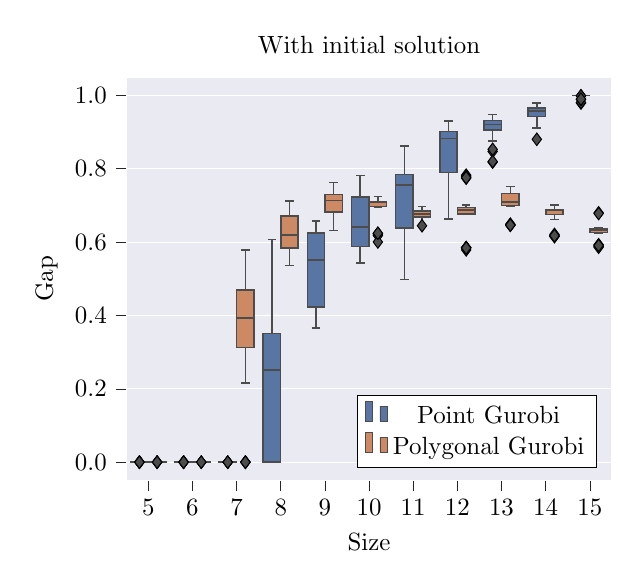
\begin{tikzpicture}[scale=0.9]

\definecolor{color0}{rgb}{0.917647058823529,0.917647058823529,0.949019607843137}
\definecolor{color1}{rgb}{0.347058823529412,0.458823529411765,0.641176470588235}
\definecolor{color2}{rgb}{0.798529411764706,0.536764705882353,0.389705882352941}

\begin{axis}[
axis background/.style={fill=color0},
axis line style={white},
tick align=outside,
title={With initial solution},
x grid style={white},
xtick pos = left,
ytick pos = left,
xlabel={Size},
% xmajorticks=false,
xmin=-0.5, xmax=10.5,
xtick style={color=white!15!black},
xtick={0,1,2,3,4,5,6,7,8,9,10},
xticklabels={5,6,7,8,9,10,11,12,13,14,15},
y grid style={white},
ylabel={Gap},
ymajorgrids,
% ymajorticks=false,
ymin=-0.05, ymax=1.05,
ytick style={color=white!15!black},
ytick={-0.2,0,0.2,0.4,0.6,0.8,1,1.2},
yticklabels={−0.2,0.0,0.2,0.4,0.6,0.8,1.0,1.2},
legend pos = south east
]
\path [draw=white!29.8039215686275!black, fill=color1, semithick]
(axis cs:-0.396,0)
--(axis cs:-0.004,0)
--(axis cs:-0.004,1.47310892137565e-06)
--(axis cs:-0.396,1.47310892137565e-06)
--(axis cs:-0.396,0)
--cycle;
\path [draw=white!29.8039215686275!black, fill=color2, semithick]
(axis cs:0.004,2.77774835246927e-09)
--(axis cs:0.396,2.77774835246927e-09)
--(axis cs:0.396,9.44481807583901e-07)
--(axis cs:0.004,9.44481807583901e-07)
--(axis cs:0.004,2.77774835246927e-09)
--cycle;
\path [draw=white!29.8039215686275!black, fill=color1, semithick]
(axis cs:0.604,9.10555048450326e-09)
--(axis cs:0.996,9.10555048450326e-09)
--(axis cs:0.996,1.19399727940805e-07)
--(axis cs:0.604,1.19399727940805e-07)
--(axis cs:0.604,9.10555048450326e-09)
--cycle;
\path [draw=white!29.8039215686275!black, fill=color2, semithick]
(axis cs:1.004,7.65308911002938e-09)
--(axis cs:1.396,7.65308911002938e-09)
--(axis cs:1.396,1.04921941526862e-06)
--(axis cs:1.004,1.04921941526862e-06)
--(axis cs:1.004,7.65308911002938e-09)
--cycle;
\path [draw=white!29.8039215686275!black, fill=color1, semithick]
(axis cs:1.604,1.17585281204778e-08)
--(axis cs:1.996,1.17585281204778e-08)
--(axis cs:1.996,4.35838130055032e-07)
--(axis cs:1.604,4.35838130055032e-07)
--(axis cs:1.604,1.17585281204778e-08)
--cycle;
\path [draw=white!29.8039215686275!black, fill=color2, semithick]
(axis cs:2.004,0.313256682139162)
--(axis cs:2.396,0.313256682139162)
--(axis cs:2.396,0.469156736256413)
--(axis cs:2.004,0.469156736256413)
--(axis cs:2.004,0.313256682139162)
--cycle;
\path [draw=white!29.8039215686275!black, fill=color1, semithick]
(axis cs:2.604,2.30867382644028e-07)
--(axis cs:2.996,2.30867382644028e-07)
--(axis cs:2.996,0.351350494279072)
--(axis cs:2.604,0.351350494279072)
--(axis cs:2.604,2.30867382644028e-07)
--cycle;
\path [draw=white!29.8039215686275!black, fill=color2, semithick]
(axis cs:3.004,0.583297259551904)
--(axis cs:3.396,0.583297259551904)
--(axis cs:3.396,0.671522249690064)
--(axis cs:3.004,0.671522249690064)
--(axis cs:3.004,0.583297259551904)
--cycle;
\path [draw=white!29.8039215686275!black, fill=color1, semithick]
(axis cs:3.604,0.422921386954822)
--(axis cs:3.996,0.422921386954822)
--(axis cs:3.996,0.625186009811415)
--(axis cs:3.604,0.625186009811415)
--(axis cs:3.604,0.422921386954822)
--cycle;
\path [draw=white!29.8039215686275!black, fill=color2, semithick]
(axis cs:4.004,0.682605233383727)
--(axis cs:4.396,0.682605233383727)
--(axis cs:4.396,0.729601252167091)
--(axis cs:4.004,0.729601252167091)
--(axis cs:4.004,0.682605233383727)
--cycle;
\path [draw=white!29.8039215686275!black, fill=color1, semithick]
(axis cs:4.604,0.588436578228431)
--(axis cs:4.996,0.588436578228431)
--(axis cs:4.996,0.722257165758196)
--(axis cs:4.604,0.722257165758196)
--(axis cs:4.604,0.588436578228431)
--cycle;
\path [draw=white!29.8039215686275!black, fill=color2, semithick]
(axis cs:5.004,0.696675498210739)
--(axis cs:5.396,0.696675498210739)
--(axis cs:5.396,0.711194527272903)
--(axis cs:5.004,0.711194527272903)
--(axis cs:5.004,0.696675498210739)
--cycle;
\path [draw=white!29.8039215686275!black, fill=color1, semithick]
(axis cs:5.604,0.638910374443127)
--(axis cs:5.996,0.638910374443127)
--(axis cs:5.996,0.784571151233962)
--(axis cs:5.604,0.784571151233962)
--(axis cs:5.604,0.638910374443127)
--cycle;
\path [draw=white!29.8039215686275!black, fill=color2, semithick]
(axis cs:6.004,0.668956498690451)
--(axis cs:6.396,0.668956498690451)
--(axis cs:6.396,0.684499521413928)
--(axis cs:6.004,0.684499521413928)
--(axis cs:6.004,0.668956498690451)
--cycle;
\path [draw=white!29.8039215686275!black, fill=color1, semithick]
(axis cs:6.604,0.789628073761807)
--(axis cs:6.996,0.789628073761807)
--(axis cs:6.996,0.901809930506889)
--(axis cs:6.604,0.901809930506889)
--(axis cs:6.604,0.789628073761807)
--cycle;
\path [draw=white!29.8039215686275!black, fill=color2, semithick]
(axis cs:7.004,0.676840720073379)
--(axis cs:7.396,0.676840720073379)
--(axis cs:7.396,0.693733662035732)
--(axis cs:7.004,0.693733662035732)
--(axis cs:7.004,0.676840720073379)
--cycle;
\path [draw=white!29.8039215686275!black, fill=color1, semithick]
(axis cs:7.604,0.90617170825011)
--(axis cs:7.996,0.90617170825011)
--(axis cs:7.996,0.930892131280505)
--(axis cs:7.604,0.930892131280505)
--(axis cs:7.604,0.90617170825011)
--cycle;
\path [draw=white!29.8039215686275!black, fill=color2, semithick]
(axis cs:8.004,0.699249616752808)
--(axis cs:8.396,0.699249616752808)
--(axis cs:8.396,0.732098544830697)
--(axis cs:8.004,0.732098544830697)
--(axis cs:8.004,0.699249616752808)
--cycle;
\path [draw=white!29.8039215686275!black, fill=color1, semithick]
(axis cs:8.604,0.942554309430122)
--(axis cs:8.996,0.942554309430122)
--(axis cs:8.996,0.965291065368416)
--(axis cs:8.604,0.965291065368416)
--(axis cs:8.604,0.942554309430122)
--cycle;
\path [draw=white!29.8039215686275!black, fill=color2, semithick]
(axis cs:9.004,0.675757570879794)
--(axis cs:9.396,0.675757570879794)
--(axis cs:9.396,0.688668248309925)
--(axis cs:9.004,0.688668248309925)
--(axis cs:9.004,0.675757570879794)
--cycle;
\path [draw=white!29.8039215686275!black, fill=color1, semithick]
(axis cs:9.604,1)
--(axis cs:9.996,1)
--(axis cs:9.996,1)
--(axis cs:9.604,1)
--(axis cs:9.604,1)
--cycle;
\path [draw=white!29.8039215686275!black, fill=color2, semithick]
(axis cs:10.004,0.62571903360804)
--(axis cs:10.396,0.62571903360804)
--(axis cs:10.396,0.63662665159059)
--(axis cs:10.004,0.63662665159059)
--(axis cs:10.004,0.62571903360804)
--cycle;
\draw[draw=white!29.8039215686275!black,fill=color1,line width=0.3pt] (axis cs:0,0) rectangle (axis cs:0,0);
\addlegendimage{ybar,ybar legend,draw=white!29.8039215686275!black,fill=color1,line width=0.3pt}
\addlegendentry{Point Gurobi}

\draw[draw=white!29.8039215686275!black,fill=color2,line width=0.3pt] (axis cs:0,0) rectangle (axis cs:0,0);
\addlegendimage{ybar,ybar legend,draw=white!29.8039215686275!black,fill=color2,line width=0.3pt}
\addlegendentry{Polygonal Gurobi}

\addplot [semithick, white!29.8039215686275!black]
table {%
-0.2 0
-0.2 0
};
\addplot [semithick, white!29.8039215686275!black]
table {%
-0.2 1.47310892137565e-06
-0.2 1.70053680170047e-06
};
\addplot [semithick, white!29.8039215686275!black]
table {%
-0.298 0
-0.102 0
};
\addplot [semithick, white!29.8039215686275!black]
table {%
-0.298 1.70053680170047e-06
-0.102 1.70053680170047e-06
};
\addplot [black, mark=diamond*, mark size=2.5, mark options={solid,fill=white!29.8039215686275!black}, only marks]
table {%
-0.2 1.35381695780653e-05
-0.2 5.32877521969958e-05
-0.2 8.05781230070993e-05
-0.2 2.25804884183551e-05
-0.2 5.09066645978979e-06
};
\addplot [semithick, white!29.8039215686275!black]
table {%
0.2 2.77774835246927e-09
0.2 0
};
\addplot [semithick, white!29.8039215686275!black]
table {%
0.2 9.44481807583901e-07
0.2 1.32298661826542e-06
};
\addplot [semithick, white!29.8039215686275!black]
table {%
0.102 0
0.298 0
};
\addplot [semithick, white!29.8039215686275!black]
table {%
0.102 1.32298661826542e-06
0.298 1.32298661826542e-06
};
\addplot [black, mark=diamond*, mark size=2.5, mark options={solid,fill=white!29.8039215686275!black}, only marks]
table {%
0.2 5.21006015712029e-06
0.2 3.76087079820426e-06
0.2 3.94677796505576e-05
0.2 8.34496385290933e-05
};
\addplot [semithick, white!29.8039215686275!black]
table {%
0.8 9.10555048450326e-09
0.8 0
};
\addplot [semithick, white!29.8039215686275!black]
table {%
0.8 1.19399727940805e-07
0.8 1.19399727940805e-07
};
\addplot [semithick, white!29.8039215686275!black]
table {%
0.702 0
0.898 0
};
\addplot [semithick, white!29.8039215686275!black]
table {%
0.702 1.19399727940805e-07
0.898 1.19399727940805e-07
};
\addplot [black, mark=diamond*, mark size=2.5, mark options={solid,fill=white!29.8039215686275!black}, only marks]
table {%
0.8 9.59689138853021e-07
0.8 5.63919624534666e-06
0.8 3.98189580024089e-06
0.8 3.74215520092297e-07
0.8 7.85986139178192e-06
0.8 1.23492347646251e-05
};
\addplot [semithick, white!29.8039215686275!black]
table {%
1.2 7.65308911002938e-09
1.2 0
};
\addplot [semithick, white!29.8039215686275!black]
table {%
1.2 1.04921941526862e-06
1.2 1.47400442150587e-06
};
\addplot [semithick, white!29.8039215686275!black]
table {%
1.102 0
1.298 0
};
\addplot [semithick, white!29.8039215686275!black]
table {%
1.102 1.47400442150587e-06
1.298 1.47400442150587e-06
};
\addplot [black, mark=diamond*, mark size=2.5, mark options={solid,fill=white!29.8039215686275!black}, only marks]
table {%
1.2 2.92264484267872e-06
1.2 2.39393028369459e-05
1.2 7.37835826296178e-05
};
\addplot [semithick, white!29.8039215686275!black]
table {%
1.8 1.17585281204778e-08
1.8 0
};
\addplot [semithick, white!29.8039215686275!black]
table {%
1.8 4.35838130055032e-07
1.8 8.12358510076968e-07
};
\addplot [semithick, white!29.8039215686275!black]
table {%
1.702 0
1.898 0
};
\addplot [semithick, white!29.8039215686275!black]
table {%
1.702 8.12358510076968e-07
1.898 8.12358510076968e-07
};
\addplot [black, mark=diamond*, mark size=2.5, mark options={solid,fill=white!29.8039215686275!black}, only marks]
table {%
1.8 1.5995012052164e-06
1.8 2.88715361710891e-05
1.8 1.50527834413872e-05
1.8 5.44315320840887e-06
};
\addplot [semithick, white!29.8039215686275!black]
table {%
2.2 0.313256682139162
2.2 0.215846215248183
};
\addplot [semithick, white!29.8039215686275!black]
table {%
2.2 0.469156736256413
2.2 0.578751459336406
};
\addplot [semithick, white!29.8039215686275!black]
table {%
2.102 0.215846215248183
2.298 0.215846215248183
};
\addplot [semithick, white!29.8039215686275!black]
table {%
2.102 0.578751459336406
2.298 0.578751459336406
};
\addplot [black, mark=diamond*, mark size=2.5, mark options={solid,fill=white!29.8039215686275!black}, only marks]
table {%
2.2 4.90170752664652e-06
2.2 6.86027673802938e-05
2.2 0
2.2 9.23373906115479e-10
};
\addplot [semithick, white!29.8039215686275!black]
table {%
2.8 2.30867382644028e-07
2.8 0
};
\addplot [semithick, white!29.8039215686275!black]
table {%
2.8 0.351350494279072
2.8 0.606844362780089
};
\addplot [semithick, white!29.8039215686275!black]
table {%
2.702 0
2.898 0
};
\addplot [semithick, white!29.8039215686275!black]
table {%
2.702 0.606844362780089
2.898 0.606844362780089
};
\addplot [semithick, white!29.8039215686275!black]
table {%
3.2 0.583297259551904
3.2 0.53630683098447
};
\addplot [semithick, white!29.8039215686275!black]
table {%
3.2 0.671522249690064
3.2 0.712064892880936
};
\addplot [semithick, white!29.8039215686275!black]
table {%
3.102 0.53630683098447
3.298 0.53630683098447
};
\addplot [semithick, white!29.8039215686275!black]
table {%
3.102 0.712064892880936
3.298 0.712064892880936
};
\addplot [semithick, white!29.8039215686275!black]
table {%
3.8 0.422921386954822
3.8 0.365661045068991
};
\addplot [semithick, white!29.8039215686275!black]
table {%
3.8 0.625186009811415
3.8 0.657898312009179
};
\addplot [semithick, white!29.8039215686275!black]
table {%
3.702 0.365661045068991
3.898 0.365661045068991
};
\addplot [semithick, white!29.8039215686275!black]
table {%
3.702 0.657898312009179
3.898 0.657898312009179
};
\addplot [semithick, white!29.8039215686275!black]
table {%
4.2 0.682605233383727
4.2 0.6318132131685
};
\addplot [semithick, white!29.8039215686275!black]
table {%
4.2 0.729601252167091
4.2 0.762691090007046
};
\addplot [semithick, white!29.8039215686275!black]
table {%
4.102 0.6318132131685
4.298 0.6318132131685
};
\addplot [semithick, white!29.8039215686275!black]
table {%
4.102 0.762691090007046
4.298 0.762691090007046
};
\addplot [semithick, white!29.8039215686275!black]
table {%
4.8 0.588436578228431
4.8 0.543400551304206
};
\addplot [semithick, white!29.8039215686275!black]
table {%
4.8 0.722257165758196
4.8 0.781492171981855
};
\addplot [semithick, white!29.8039215686275!black]
table {%
4.702 0.543400551304206
4.898 0.543400551304206
};
\addplot [semithick, white!29.8039215686275!black]
table {%
4.702 0.781492171981855
4.898 0.781492171981855
};
\addplot [semithick, white!29.8039215686275!black]
table {%
5.2 0.696675498210739
5.2 0.695804401495872
};
\addplot [semithick, white!29.8039215686275!black]
table {%
5.2 0.711194527272903
5.2 0.724766380000275
};
\addplot [semithick, white!29.8039215686275!black]
table {%
5.102 0.695804401495872
5.298 0.695804401495872
};
\addplot [semithick, white!29.8039215686275!black]
table {%
5.102 0.724766380000275
5.298 0.724766380000275
};
\addplot [black, mark=diamond*, mark size=2.5, mark options={solid,fill=white!29.8039215686275!black}, only marks]
table {%
5.2 0.621621854751754
5.2 0.617782362510201
5.2 0.623807308761354
5.2 0.600297180424914
5.2 0.624032332802482
};
\addplot [semithick, white!29.8039215686275!black]
table {%
5.8 0.638910374443127
5.8 0.498590337234061
};
\addplot [semithick, white!29.8039215686275!black]
table {%
5.8 0.784571151233962
5.8 0.861883164147105
};
\addplot [semithick, white!29.8039215686275!black]
table {%
5.702 0.498590337234061
5.898 0.498590337234061
};
\addplot [semithick, white!29.8039215686275!black]
table {%
5.702 0.861883164147105
5.898 0.861883164147105
};
\addplot [semithick, white!29.8039215686275!black]
table {%
6.2 0.668956498690451
6.2 0.646587509676844
};
\addplot [semithick, white!29.8039215686275!black]
table {%
6.2 0.684499521413928
6.2 0.697264500175136
};
\addplot [semithick, white!29.8039215686275!black]
table {%
6.102 0.646587509676844
6.298 0.646587509676844
};
\addplot [semithick, white!29.8039215686275!black]
table {%
6.102 0.697264500175136
6.298 0.697264500175136
};
\addplot [black, mark=diamond*, mark size=2.5, mark options={solid,fill=white!29.8039215686275!black}, only marks]
table {%
6.2 0.644480415436732
};
\addplot [semithick, white!29.8039215686275!black]
table {%
6.8 0.789628073761807
6.8 0.662949357287658
};
\addplot [semithick, white!29.8039215686275!black]
table {%
6.8 0.901809930506889
6.8 0.929916802365185
};
\addplot [semithick, white!29.8039215686275!black]
table {%
6.702 0.662949357287658
6.898 0.662949357287658
};
\addplot [semithick, white!29.8039215686275!black]
table {%
6.702 0.929916802365185
6.898 0.929916802365185
};
\addplot [semithick, white!29.8039215686275!black]
table {%
7.2 0.676840720073379
7.2 0.675350397777501
};
\addplot [semithick, white!29.8039215686275!black]
table {%
7.2 0.693733662035732
7.2 0.700518970314745
};
\addplot [semithick, white!29.8039215686275!black]
table {%
7.102 0.675350397777501
7.298 0.675350397777501
};
\addplot [semithick, white!29.8039215686275!black]
table {%
7.102 0.700518970314745
7.298 0.700518970314745
};
\addplot [black, mark=diamond*, mark size=2.5, mark options={solid,fill=white!29.8039215686275!black}, only marks]
table {%
7.2 0.578607197836962
7.2 0.584592616847172
7.2 0.584929948739234
7.2 0.584815266176306
7.2 0.583930741899315
7.2 0.782404947450128
7.2 0.777258909995048
7.2 0.779874965633844
7.2 0.774108355382069
7.2 0.775585116921516
};
\addplot [semithick, white!29.8039215686275!black]
table {%
7.8 0.90617170825011
7.8 0.875944764311254
};
\addplot [semithick, white!29.8039215686275!black]
table {%
7.8 0.930892131280505
7.8 0.947542409296488
};
\addplot [semithick, white!29.8039215686275!black]
table {%
7.702 0.875944764311254
7.898 0.875944764311254
};
\addplot [semithick, white!29.8039215686275!black]
table {%
7.702 0.947542409296488
7.898 0.947542409296488
};
\addplot [black, mark=diamond*, mark size=2.5, mark options={solid,fill=white!29.8039215686275!black}, only marks]
table {%
7.8 0.847133767496126
7.8 0.817934678492407
7.8 0.819561079339476
7.8 0.852955691161731
};
\addplot [semithick, white!29.8039215686275!black]
table {%
8.2 0.699249616752808
8.2 0.698928009847033
};
\addplot [semithick, white!29.8039215686275!black]
table {%
8.2 0.732098544830697
8.2 0.75196324551946
};
\addplot [semithick, white!29.8039215686275!black]
table {%
8.102 0.698928009847033
8.298 0.698928009847033
};
\addplot [semithick, white!29.8039215686275!black]
table {%
8.102 0.75196324551946
8.298 0.75196324551946
};
\addplot [black, mark=diamond*, mark size=2.5, mark options={solid,fill=white!29.8039215686275!black}, only marks]
table {%
8.2 0.64639641904659
8.2 0.646913911191774
8.2 0.648844716299477
8.2 0.645928411019802
8.2 0.646253923707761
};
\addplot [semithick, white!29.8039215686275!black]
table {%
8.8 0.942554309430122
8.8 0.911636275270979
};
\addplot [semithick, white!29.8039215686275!black]
table {%
8.8 0.965291065368416
8.8 0.978985763193375
};
\addplot [semithick, white!29.8039215686275!black]
table {%
8.702 0.911636275270979
8.898 0.911636275270979
};
\addplot [semithick, white!29.8039215686275!black]
table {%
8.702 0.978985763193375
8.898 0.978985763193375
};
\addplot [black, mark=diamond*, mark size=2.5, mark options={solid,fill=white!29.8039215686275!black}, only marks]
table {%
8.8 0.880186013927618
};
\addplot [semithick, white!29.8039215686275!black]
table {%
9.2 0.675757570879794
9.2 0.660951425716328
};
\addplot [semithick, white!29.8039215686275!black]
table {%
9.2 0.688668248309925
9.2 0.700814385688795
};
\addplot [semithick, white!29.8039215686275!black]
table {%
9.102 0.660951425716328
9.298 0.660951425716328
};
\addplot [semithick, white!29.8039215686275!black]
table {%
9.102 0.700814385688795
9.298 0.700814385688795
};
\addplot [black, mark=diamond*, mark size=2.5, mark options={solid,fill=white!29.8039215686275!black}, only marks]
table {%
9.2 0.615695557216502
9.2 0.617449525502551
9.2 0.614856603992895
9.2 0.620890877643559
9.2 0.617449502132708
};
\addplot [semithick, white!29.8039215686275!black]
table {%
9.8 1
9.8 1
};
\addplot [semithick, white!29.8039215686275!black]
table {%
9.8 1
9.8 1
};
\addplot [semithick, white!29.8039215686275!black]
table {%
9.702 1
9.898 1
};
\addplot [semithick, white!29.8039215686275!black]
table {%
9.702 1
9.898 1
};
\addplot [black, mark=diamond*, mark size=2.5, mark options={solid,fill=white!29.8039215686275!black}, only marks]
table {%
9.8 0.97907124998238
9.8 0.980653787500368
9.8 0.988792265674311
9.8 0.99851904524003
9.8 0.998647261723464
9.8 0.989829745517829
};
\addplot [semithick, white!29.8039215686275!black]
table {%
10.2 0.62571903360804
10.2 0.625247605867215
};
\addplot [semithick, white!29.8039215686275!black]
table {%
10.2 0.63662665159059
10.2 0.63928107592984
};
\addplot [semithick, white!29.8039215686275!black]
table {%
10.102 0.625247605867215
10.298 0.625247605867215
};
\addplot [semithick, white!29.8039215686275!black]
table {%
10.102 0.63928107592984
10.298 0.63928107592984
};
\addplot [black, mark=diamond*, mark size=2.5, mark options={solid,fill=white!29.8039215686275!black}, only marks]
table {%
10.2 0.589711757089996
10.2 0.588095037209433
10.2 0.585879604451199
10.2 0.592868929598296
10.2 0.590630766181204
10.2 0.679665124462296
10.2 0.677718806087101
};
\addplot [semithick, white!29.8039215686275!black]
table {%
-0.396 3.4978630333614e-09
-0.004 3.4978630333614e-09
};
\addplot [semithick, white!29.8039215686275!black]
table {%
0.004 7.5047702830497e-08
0.396 7.5047702830497e-08
};
\addplot [semithick, white!29.8039215686275!black]
table {%
0.604 3.55689804933838e-08
0.996 3.55689804933838e-08
};
\addplot [semithick, white!29.8039215686275!black]
table {%
1.004 3.15970508806205e-07
1.396 3.15970508806205e-07
};
\addplot [semithick, white!29.8039215686275!black]
table {%
1.604 3.60766817512181e-08
1.996 3.60766817512181e-08
};
\addplot [semithick, white!29.8039215686275!black]
table {%
2.004 0.392577289964846
2.396 0.392577289964846
};
\addplot [semithick, white!29.8039215686275!black]
table {%
2.604 0.251215981686063
2.996 0.251215981686063
};
\addplot [semithick, white!29.8039215686275!black]
table {%
3.004 0.619171721623484
3.396 0.619171721623484
};
\addplot [semithick, white!29.8039215686275!black]
table {%
3.604 0.551595792131333
3.996 0.551595792131333
};
\addplot [semithick, white!29.8039215686275!black]
table {%
4.004 0.713334875473806
4.396 0.713334875473806
};
\addplot [semithick, white!29.8039215686275!black]
table {%
4.604 0.64134352700276
4.996 0.64134352700276
};
\addplot [semithick, white!29.8039215686275!black]
table {%
5.004 0.707629610395339
5.396 0.707629610395339
};
\addplot [semithick, white!29.8039215686275!black]
table {%
5.604 0.756192081981762
5.996 0.756192081981762
};
\addplot [semithick, white!29.8039215686275!black]
table {%
6.004 0.677009397005272
6.396 0.677009397005272
};
\addplot [semithick, white!29.8039215686275!black]
table {%
6.604 0.881973438607248
6.996 0.881973438607248
};
\addplot [semithick, white!29.8039215686275!black]
table {%
7.004 0.687240210845712
7.396 0.687240210845712
};
\addplot [semithick, white!29.8039215686275!black]
table {%
7.604 0.920928153870394
7.996 0.920928153870394
};
\addplot [semithick, white!29.8039215686275!black]
table {%
8.004 0.709493668226716
8.396 0.709493668226716
};
\addplot [semithick, white!29.8039215686275!black]
table {%
8.604 0.957960682284585
8.996 0.957960682284585
};
\addplot [semithick, white!29.8039215686275!black]
table {%
9.004 0.687565982773435
9.396 0.687565982773435
};
\addplot [semithick, white!29.8039215686275!black]
table {%
9.604 1
9.996 1
};
\addplot [semithick, white!29.8039215686275!black]
table {%
10.004 0.632483367113265
10.396 0.632483367113265
};
\end{axis}

\end{tikzpicture}


\caption{Final gap with and without initialization by using Gurobi.}
\label{fig:Fig4}
\end{figure}

% \DeclareUnicodeCharacter{2212}{−}
\usetikzlibrary{patterns,shapes.arrows}
\pgfplotsset{compat=newest}

\begin{figure}
    \centering
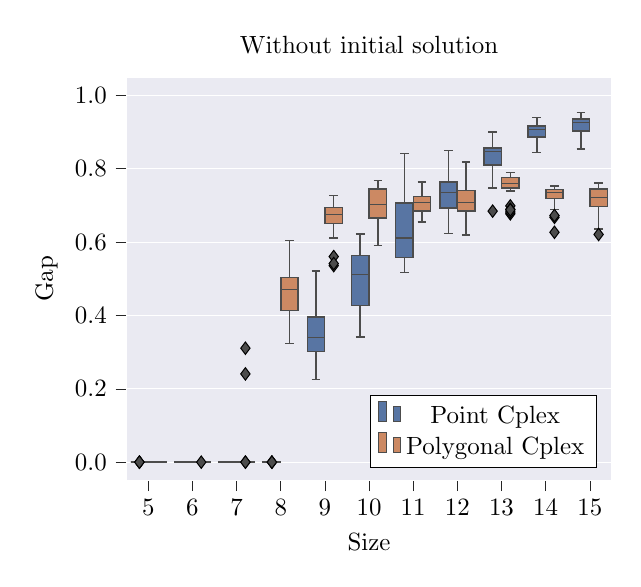
\begin{tikzpicture}[scale=0.9]

\definecolor{color0}{rgb}{0.917647058823529,0.917647058823529,0.949019607843137}
\definecolor{color1}{rgb}{0.347058823529412,0.458823529411765,0.641176470588235}
\definecolor{color2}{rgb}{0.798529411764706,0.536764705882353,0.389705882352941}

\begin{axis}[
axis background/.style={fill=color0},
axis line style={white},
tick align=outside,
title={Without initial solution},
x grid style={white},
xtick pos = left,
ytick pos = left,
xlabel={Size},
% xmajorticks=false,
xmin=-0.5, xmax=10.5,
xtick style={color=white!15!black},
xtick={0,1,2,3,4,5,6,7,8,9,10},
xticklabels={5,6,7,8,9,10,11,12,13,14,15},
y grid style={white},
ylabel={Gap},
ymajorgrids,
% ymajorticks=false,
ymin=-0.05, ymax=1.05,
ytick style={color=white!15!black},
ytick={-0.2,0,0.2,0.4,0.6,0.8,1,1.2},
yticklabels={−0.2,0.0,0.2,0.4,0.6,0.8,1.0,1.2},
legend pos = south east
]
\path [draw=white!29.8039215686275!black, fill=color1, semithick]
(axis cs:-0.396,0)
--(axis cs:-0.004,0)
--(axis cs:-0.004,0)
--(axis cs:-0.396,0)
--(axis cs:-0.396,0)
--cycle;
\path [draw=white!29.8039215686275!black, fill=color2, semithick]
(axis cs:0.004,0)
--(axis cs:0.396,0)
--(axis cs:0.396,7.27025579647183e-05)
--(axis cs:0.004,7.27025579647183e-05)
--(axis cs:0.004,0)
--cycle;
\path [draw=white!29.8039215686275!black, fill=color1, semithick]
(axis cs:0.604,0)
--(axis cs:0.996,0)
--(axis cs:0.996,4.87038618912926e-05)
--(axis cs:0.604,4.87038618912926e-05)
--(axis cs:0.604,0)
--cycle;
\path [draw=white!29.8039215686275!black, fill=color2, semithick]
(axis cs:1.004,5.4563466300783e-05)
--(axis cs:1.396,5.4563466300783e-05)
--(axis cs:1.396,8.5592993766572e-05)
--(axis cs:1.004,8.5592993766572e-05)
--(axis cs:1.004,5.4563466300783e-05)
--cycle;
\path [draw=white!29.8039215686275!black, fill=color1, semithick]
(axis cs:1.604,2.2523387185749e-05)
--(axis cs:1.996,2.2523387185749e-05)
--(axis cs:1.996,9.26447708859183e-05)
--(axis cs:1.604,9.26447708859183e-05)
--(axis cs:1.604,2.2523387185749e-05)
--cycle;
\path [draw=white!29.8039215686275!black, fill=color2, semithick]
(axis cs:2.004,9.08925141411829e-05)
--(axis cs:2.396,9.08925141411829e-05)
--(axis cs:2.396,9.92772438608017e-05)
--(axis cs:2.004,9.92772438608017e-05)
--(axis cs:2.004,9.08925141411829e-05)
--cycle;
\path [draw=white!29.8039215686275!black, fill=color1, semithick]
(axis cs:2.604,9.36992758361936e-05)
--(axis cs:2.996,9.36992758361936e-05)
--(axis cs:2.996,9.8387119197486e-05)
--(axis cs:2.604,9.8387119197486e-05)
--(axis cs:2.604,9.36992758361936e-05)
--cycle;
\path [draw=white!29.8039215686275!black, fill=color2, semithick]
(axis cs:3.004,0.412897054547102)
--(axis cs:3.396,0.412897054547102)
--(axis cs:3.396,0.503605725234685)
--(axis cs:3.004,0.503605725234685)
--(axis cs:3.004,0.412897054547102)
--cycle;
\path [draw=white!29.8039215686275!black, fill=color1, semithick]
(axis cs:3.604,0.302279475411954)
--(axis cs:3.996,0.302279475411954)
--(axis cs:3.996,0.395328744222783)
--(axis cs:3.604,0.395328744222783)
--(axis cs:3.604,0.302279475411954)
--cycle;
\path [draw=white!29.8039215686275!black, fill=color2, semithick]
(axis cs:4.004,0.650992665233004)
--(axis cs:4.396,0.650992665233004)
--(axis cs:4.396,0.693580884653997)
--(axis cs:4.004,0.693580884653997)
--(axis cs:4.004,0.650992665233004)
--cycle;
\path [draw=white!29.8039215686275!black, fill=color1, semithick]
(axis cs:4.604,0.426815371358812)
--(axis cs:4.996,0.426815371358812)
--(axis cs:4.996,0.563187996252681)
--(axis cs:4.604,0.563187996252681)
--(axis cs:4.604,0.426815371358812)
--cycle;
\path [draw=white!29.8039215686275!black, fill=color2, semithick]
(axis cs:5.004,0.66494903292594)
--(axis cs:5.396,0.66494903292594)
--(axis cs:5.396,0.744635483351167)
--(axis cs:5.004,0.744635483351167)
--(axis cs:5.004,0.66494903292594)
--cycle;
\path [draw=white!29.8039215686275!black, fill=color1, semithick]
(axis cs:5.604,0.557404615074999)
--(axis cs:5.996,0.557404615074999)
--(axis cs:5.996,0.706452416984265)
--(axis cs:5.604,0.706452416984265)
--(axis cs:5.604,0.557404615074999)
--cycle;
\path [draw=white!29.8039215686275!black, fill=color2, semithick]
(axis cs:6.004,0.685265561441549)
--(axis cs:6.396,0.685265561441549)
--(axis cs:6.396,0.723654575397984)
--(axis cs:6.004,0.723654575397984)
--(axis cs:6.004,0.685265561441549)
--cycle;
\path [draw=white!29.8039215686275!black, fill=color1, semithick]
(axis cs:6.604,0.69227945285344)
--(axis cs:6.996,0.69227945285344)
--(axis cs:6.996,0.764242981948201)
--(axis cs:6.604,0.764242981948201)
--(axis cs:6.604,0.69227945285344)
--cycle;
\path [draw=white!29.8039215686275!black, fill=color2, semithick]
(axis cs:7.004,0.684426855287346)
--(axis cs:7.396,0.684426855287346)
--(axis cs:7.396,0.740744625099486)
--(axis cs:7.004,0.740744625099486)
--(axis cs:7.004,0.684426855287346)
--cycle;
\path [draw=white!29.8039215686275!black, fill=color1, semithick]
(axis cs:7.604,0.809707964402874)
--(axis cs:7.996,0.809707964402874)
--(axis cs:7.996,0.856347510716666)
--(axis cs:7.604,0.856347510716666)
--(axis cs:7.604,0.809707964402874)
--cycle;
\path [draw=white!29.8039215686275!black, fill=color2, semithick]
(axis cs:8.004,0.747565302096636)
--(axis cs:8.396,0.747565302096636)
--(axis cs:8.396,0.776465307150937)
--(axis cs:8.004,0.776465307150937)
--(axis cs:8.004,0.747565302096636)
--cycle;
\path [draw=white!29.8039215686275!black, fill=color1, semithick]
(axis cs:8.604,0.886961612437911)
--(axis cs:8.996,0.886961612437911)
--(axis cs:8.996,0.916160241323283)
--(axis cs:8.604,0.916160241323283)
--(axis cs:8.604,0.886961612437911)
--cycle;
\path [draw=white!29.8039215686275!black, fill=color2, semithick]
(axis cs:9.004,0.719174723055696)
--(axis cs:9.396,0.719174723055696)
--(axis cs:9.396,0.743421800811077)
--(axis cs:9.004,0.743421800811077)
--(axis cs:9.004,0.719174723055696)
--cycle;
\path [draw=white!29.8039215686275!black, fill=color1, semithick]
(axis cs:9.604,0.902152649649257)
--(axis cs:9.996,0.902152649649257)
--(axis cs:9.996,0.935411833777553)
--(axis cs:9.604,0.935411833777553)
--(axis cs:9.604,0.902152649649257)
--cycle;
\path [draw=white!29.8039215686275!black, fill=color2, semithick]
(axis cs:10.004,0.696796392404108)
--(axis cs:10.396,0.696796392404108)
--(axis cs:10.396,0.745316195446882)
--(axis cs:10.004,0.745316195446882)
--(axis cs:10.004,0.696796392404108)
--cycle;
\draw[draw=white!29.8039215686275!black,fill=color1,line width=0.3pt] (axis cs:0,0) rectangle (axis cs:0,0);
\addlegendimage{ybar,ybar legend,draw=white!29.8039215686275!black,fill=color1,line width=0.3pt}
\addlegendentry{Point Cplex}

\draw[draw=white!29.8039215686275!black,fill=color2,line width=0.3pt] (axis cs:0,0) rectangle (axis cs:0,0);
\addlegendimage{ybar,ybar legend,draw=white!29.8039215686275!black,fill=color2,line width=0.3pt}
\addlegendentry{Polygonal Cplex}

\addplot [semithick, white!29.8039215686275!black]
table {%
-0.2 0
-0.2 0
};
\addplot [semithick, white!29.8039215686275!black]
table {%
-0.2 0
-0.2 0
};
\addplot [semithick, white!29.8039215686275!black]
table {%
-0.298 0
-0.102 0
};
\addplot [semithick, white!29.8039215686275!black]
table {%
-0.298 0
-0.102 0
};
\addplot [black, mark=diamond*, mark size=2.5, mark options={solid,fill=white!29.8039215686275!black}, only marks]
table {%
-0.2 2.05706758576122e-07
-0.2 1.50366414660575e-05
-0.2 6.3648789644588e-05
};
\addplot [semithick, white!29.8039215686275!black]
table {%
0.2 0
0.2 0
};
\addplot [semithick, white!29.8039215686275!black]
table {%
0.2 7.27025579647183e-05
0.2 9.68144899643098e-05
};
\addplot [semithick, white!29.8039215686275!black]
table {%
0.102 0
0.298 0
};
\addplot [semithick, white!29.8039215686275!black]
table {%
0.102 9.68144899643098e-05
0.298 9.68144899643098e-05
};
\addplot [semithick, white!29.8039215686275!black]
table {%
0.8 0
0.8 0
};
\addplot [semithick, white!29.8039215686275!black]
table {%
0.8 4.87038618912926e-05
0.8 9.12125484854416e-05
};
\addplot [semithick, white!29.8039215686275!black]
table {%
0.702 0
0.898 0
};
\addplot [semithick, white!29.8039215686275!black]
table {%
0.702 9.12125484854416e-05
0.898 9.12125484854416e-05
};
\addplot [semithick, white!29.8039215686275!black]
table {%
1.2 5.4563466300783e-05
1.2 3.16525355461071e-05
};
\addplot [semithick, white!29.8039215686275!black]
table {%
1.2 8.5592993766572e-05
1.2 9.57930399770383e-05
};
\addplot [semithick, white!29.8039215686275!black]
table {%
1.102 3.16525355461071e-05
1.298 3.16525355461071e-05
};
\addplot [semithick, white!29.8039215686275!black]
table {%
1.102 9.57930399770383e-05
1.298 9.57930399770383e-05
};
\addplot [black, mark=diamond*, mark size=2.5, mark options={solid,fill=white!29.8039215686275!black}, only marks]
table {%
1.2 0
};
\addplot [semithick, white!29.8039215686275!black]
table {%
1.8 2.2523387185749e-05
1.8 0
};
\addplot [semithick, white!29.8039215686275!black]
table {%
1.8 9.26447708859183e-05
1.8 9.96440668958393e-05
};
\addplot [semithick, white!29.8039215686275!black]
table {%
1.702 0
1.898 0
};
\addplot [semithick, white!29.8039215686275!black]
table {%
1.702 9.96440668958393e-05
1.898 9.96440668958393e-05
};
\addplot [semithick, white!29.8039215686275!black]
table {%
2.2 9.08925141411829e-05
2.2 8.35637743391164e-05
};
\addplot [semithick, white!29.8039215686275!black]
table {%
2.2 9.92772438608017e-05
2.2 9.97807942946948e-05
};
\addplot [semithick, white!29.8039215686275!black]
table {%
2.102 8.35637743391164e-05
2.298 8.35637743391164e-05
};
\addplot [semithick, white!29.8039215686275!black]
table {%
2.102 9.97807942946948e-05
2.298 9.97807942946948e-05
};
\addplot [black, mark=diamond*, mark size=2.5, mark options={solid,fill=white!29.8039215686275!black}, only marks]
table {%
2.2 7.69565093620003e-05
2.2 7.71987935127202e-05
2.2 0.310608844468141
2.2 0.240547964848536
};
\addplot [semithick, white!29.8039215686275!black]
table {%
2.8 9.36992758361936e-05
2.8 8.67393812443088e-05
};
\addplot [semithick, white!29.8039215686275!black]
table {%
2.8 9.8387119197486e-05
2.8 9.99763410417882e-05
};
\addplot [semithick, white!29.8039215686275!black]
table {%
2.702 8.67393812443088e-05
2.898 8.67393812443088e-05
};
\addplot [semithick, white!29.8039215686275!black]
table {%
2.702 9.99763410417882e-05
2.898 9.99763410417882e-05
};
\addplot [black, mark=diamond*, mark size=2.5, mark options={solid,fill=white!29.8039215686275!black}, only marks]
table {%
2.8 7.8649251372998e-05
2.8 8.33504100109573e-05
2.8 8.27365523673414e-05
};
\addplot [semithick, white!29.8039215686275!black]
table {%
3.2 0.412897054547102
3.2 0.324085590429452
};
\addplot [semithick, white!29.8039215686275!black]
table {%
3.2 0.503605725234685
3.2 0.604529539054347
};
\addplot [semithick, white!29.8039215686275!black]
table {%
3.102 0.324085590429452
3.298 0.324085590429452
};
\addplot [semithick, white!29.8039215686275!black]
table {%
3.102 0.604529539054347
3.298 0.604529539054347
};
\addplot [semithick, white!29.8039215686275!black]
table {%
3.8 0.302279475411954
3.8 0.225737793043267
};
\addplot [semithick, white!29.8039215686275!black]
table {%
3.8 0.395328744222783
3.8 0.520968814370186
};
\addplot [semithick, white!29.8039215686275!black]
table {%
3.702 0.225737793043267
3.898 0.225737793043267
};
\addplot [semithick, white!29.8039215686275!black]
table {%
3.702 0.520968814370186
3.898 0.520968814370186
};
\addplot [semithick, white!29.8039215686275!black]
table {%
4.2 0.650992665233004
4.2 0.610588442403033
};
\addplot [semithick, white!29.8039215686275!black]
table {%
4.2 0.693580884653997
4.2 0.727378104412863
};
\addplot [semithick, white!29.8039215686275!black]
table {%
4.102 0.610588442403033
4.298 0.610588442403033
};
\addplot [semithick, white!29.8039215686275!black]
table {%
4.102 0.727378104412863
4.298 0.727378104412863
};
\addplot [black, mark=diamond*, mark size=2.5, mark options={solid,fill=white!29.8039215686275!black}, only marks]
table {%
4.2 0.560420328395935
4.2 0.535826362555011
4.2 0.541434057140162
};
\addplot [semithick, white!29.8039215686275!black]
table {%
4.8 0.426815371358812
4.8 0.341073644365041
};
\addplot [semithick, white!29.8039215686275!black]
table {%
4.8 0.563187996252681
4.8 0.622183173190176
};
\addplot [semithick, white!29.8039215686275!black]
table {%
4.702 0.341073644365041
4.898 0.341073644365041
};
\addplot [semithick, white!29.8039215686275!black]
table {%
4.702 0.622183173190176
4.898 0.622183173190176
};
\addplot [semithick, white!29.8039215686275!black]
table {%
5.2 0.66494903292594
5.2 0.590610673885409
};
\addplot [semithick, white!29.8039215686275!black]
table {%
5.2 0.744635483351167
5.2 0.76769296188471
};
\addplot [semithick, white!29.8039215686275!black]
table {%
5.102 0.590610673885409
5.298 0.590610673885409
};
\addplot [semithick, white!29.8039215686275!black]
table {%
5.102 0.76769296188471
5.298 0.76769296188471
};
\addplot [semithick, white!29.8039215686275!black]
table {%
5.8 0.557404615074999
5.8 0.516441607753319
};
\addplot [semithick, white!29.8039215686275!black]
table {%
5.8 0.706452416984265
5.8 0.841749273444217
};
\addplot [semithick, white!29.8039215686275!black]
table {%
5.702 0.516441607753319
5.898 0.516441607753319
};
\addplot [semithick, white!29.8039215686275!black]
table {%
5.702 0.841749273444217
5.898 0.841749273444217
};
\addplot [semithick, white!29.8039215686275!black]
table {%
6.2 0.685265561441549
6.2 0.654808120425694
};
\addplot [semithick, white!29.8039215686275!black]
table {%
6.2 0.723654575397984
6.2 0.763135865522515
};
\addplot [semithick, white!29.8039215686275!black]
table {%
6.102 0.654808120425694
6.298 0.654808120425694
};
\addplot [semithick, white!29.8039215686275!black]
table {%
6.102 0.763135865522515
6.298 0.763135865522515
};
\addplot [semithick, white!29.8039215686275!black]
table {%
6.8 0.69227945285344
6.8 0.623950331168401
};
\addplot [semithick, white!29.8039215686275!black]
table {%
6.8 0.764242981948201
6.8 0.849562776250825
};
\addplot [semithick, white!29.8039215686275!black]
table {%
6.702 0.623950331168401
6.898 0.623950331168401
};
\addplot [semithick, white!29.8039215686275!black]
table {%
6.702 0.849562776250825
6.898 0.849562776250825
};
\addplot [semithick, white!29.8039215686275!black]
table {%
7.2 0.684426855287346
7.2 0.619246326359349
};
\addplot [semithick, white!29.8039215686275!black]
table {%
7.2 0.740744625099486
7.2 0.817650751184577
};
\addplot [semithick, white!29.8039215686275!black]
table {%
7.102 0.619246326359349
7.298 0.619246326359349
};
\addplot [semithick, white!29.8039215686275!black]
table {%
7.102 0.817650751184577
7.298 0.817650751184577
};
\addplot [semithick, white!29.8039215686275!black]
table {%
7.8 0.809707964402874
7.8 0.747803698646072
};
\addplot [semithick, white!29.8039215686275!black]
table {%
7.8 0.856347510716666
7.8 0.899743414742338
};
\addplot [semithick, white!29.8039215686275!black]
table {%
7.702 0.747803698646072
7.898 0.747803698646072
};
\addplot [semithick, white!29.8039215686275!black]
table {%
7.702 0.899743414742338
7.898 0.899743414742338
};
\addplot [black, mark=diamond*, mark size=2.5, mark options={solid,fill=white!29.8039215686275!black}, only marks]
table {%
7.8 0.684380518668612
};
\addplot [semithick, white!29.8039215686275!black]
table {%
8.2 0.747565302096636
8.2 0.739494646266489
};
\addplot [semithick, white!29.8039215686275!black]
table {%
8.2 0.776465307150937
8.2 0.789174636649203
};
\addplot [semithick, white!29.8039215686275!black]
table {%
8.102 0.739494646266489
8.298 0.739494646266489
};
\addplot [semithick, white!29.8039215686275!black]
table {%
8.102 0.789174636649203
8.298 0.789174636649203
};
\addplot [black, mark=diamond*, mark size=2.5, mark options={solid,fill=white!29.8039215686275!black}, only marks]
table {%
8.2 0.698640106582879
8.2 0.677011765826319
8.2 0.682056310502665
8.2 0.689310392129366
8.2 0.687791368675476
};
\addplot [semithick, white!29.8039215686275!black]
table {%
8.8 0.886961612437911
8.8 0.844311934006581
};
\addplot [semithick, white!29.8039215686275!black]
table {%
8.8 0.916160241323283
8.8 0.939785619098039
};
\addplot [semithick, white!29.8039215686275!black]
table {%
8.702 0.844311934006581
8.898 0.844311934006581
};
\addplot [semithick, white!29.8039215686275!black]
table {%
8.702 0.939785619098039
8.898 0.939785619098039
};
\addplot [semithick, white!29.8039215686275!black]
table {%
9.2 0.719174723055696
9.2 0.688538189887176
};
\addplot [semithick, white!29.8039215686275!black]
table {%
9.2 0.743421800811077
9.2 0.752225960187768
};
\addplot [semithick, white!29.8039215686275!black]
table {%
9.102 0.688538189887176
9.298 0.688538189887176
};
\addplot [semithick, white!29.8039215686275!black]
table {%
9.102 0.752225960187768
9.298 0.752225960187768
};
\addplot [black, mark=diamond*, mark size=2.5, mark options={solid,fill=white!29.8039215686275!black}, only marks]
table {%
9.2 0.667497978167803
9.2 0.672408764737592
9.2 0.626671754379948
};
\addplot [semithick, white!29.8039215686275!black]
table {%
9.8 0.902152649649257
9.8 0.853203471356631
};
\addplot [semithick, white!29.8039215686275!black]
table {%
9.8 0.935411833777553
9.8 0.953877633302632
};
\addplot [semithick, white!29.8039215686275!black]
table {%
9.702 0.853203471356631
9.898 0.853203471356631
};
\addplot [semithick, white!29.8039215686275!black]
table {%
9.702 0.953877633302632
9.898 0.953877633302632
};
\addplot [semithick, white!29.8039215686275!black]
table {%
10.2 0.696796392404108
10.2 0.635012960602927
};
\addplot [semithick, white!29.8039215686275!black]
table {%
10.2 0.745316195446882
10.2 0.761575965448512
};
\addplot [semithick, white!29.8039215686275!black]
table {%
10.102 0.635012960602927
10.298 0.635012960602927
};
\addplot [semithick, white!29.8039215686275!black]
table {%
10.102 0.761575965448512
10.298 0.761575965448512
};
\addplot [black, mark=diamond*, mark size=2.5, mark options={solid,fill=white!29.8039215686275!black}, only marks]
table {%
10.2 0.620747964710293
};
\addplot [semithick, white!29.8039215686275!black]
table {%
-0.396 0
-0.004 0
};
\addplot [semithick, white!29.8039215686275!black]
table {%
0.004 2.32234168284018e-05
0.396 2.32234168284018e-05
};
\addplot [semithick, white!29.8039215686275!black]
table {%
0.604 0
0.996 0
};
\addplot [semithick, white!29.8039215686275!black]
table {%
1.004 7.66346328030035e-05
1.396 7.66346328030035e-05
};
\addplot [semithick, white!29.8039215686275!black]
table {%
1.604 7.321056076593e-05
1.996 7.321056076593e-05
};
\addplot [semithick, white!29.8039215686275!black]
table {%
2.004 9.51047397985199e-05
2.396 9.51047397985199e-05
};
\addplot [semithick, white!29.8039215686275!black]
table {%
2.604 9.65681455578857e-05
2.996 9.65681455578857e-05
};
\addplot [semithick, white!29.8039215686275!black]
table {%
3.004 0.471224379534675
3.396 0.471224379534675
};
\addplot [semithick, white!29.8039215686275!black]
table {%
3.604 0.340171562773011
3.996 0.340171562773011
};
\addplot [semithick, white!29.8039215686275!black]
table {%
4.004 0.674982417498147
4.396 0.674982417498147
};
\addplot [semithick, white!29.8039215686275!black]
table {%
4.604 0.512246153211272
4.996 0.512246153211272
};
\addplot [semithick, white!29.8039215686275!black]
table {%
5.004 0.702799591122842
5.396 0.702799591122842
};
\addplot [semithick, white!29.8039215686275!black]
table {%
5.604 0.611223659787013
5.996 0.611223659787013
};
\addplot [semithick, white!29.8039215686275!black]
table {%
6.004 0.708042103434346
6.396 0.708042103434346
};
\addplot [semithick, white!29.8039215686275!black]
table {%
6.604 0.735716995662596
6.996 0.735716995662596
};
\addplot [semithick, white!29.8039215686275!black]
table {%
7.004 0.707936723265078
7.396 0.707936723265078
};
\addplot [semithick, white!29.8039215686275!black]
table {%
7.604 0.847152254855732
7.996 0.847152254855732
};
\addplot [semithick, white!29.8039215686275!black]
table {%
8.004 0.759953796189026
8.396 0.759953796189026
};
\addplot [semithick, white!29.8039215686275!black]
table {%
8.604 0.907349714682547
8.996 0.907349714682547
};
\addplot [semithick, white!29.8039215686275!black]
table {%
9.004 0.734647246430435
9.396 0.734647246430435
};
\addplot [semithick, white!29.8039215686275!black]
table {%
9.604 0.925762148040081
9.996 0.925762148040081
};
\addplot [semithick, white!29.8039215686275!black]
table {%
10.004 0.721311479879954
10.396 0.721311479879954
};
\end{axis}

\end{tikzpicture}
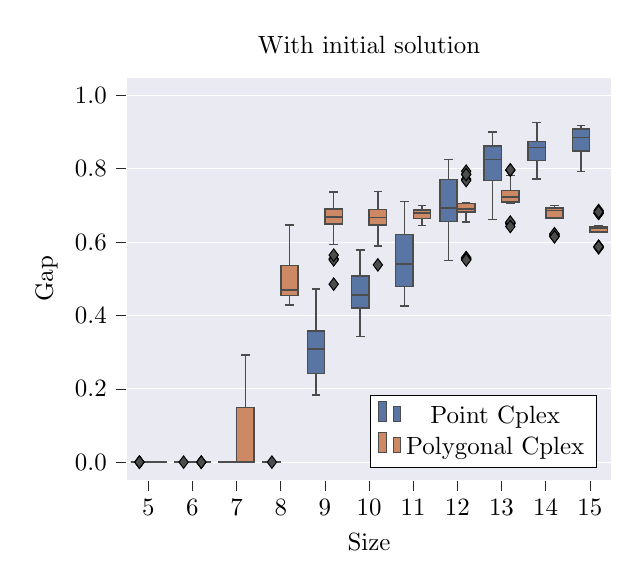
\begin{tikzpicture}[scale=0.9]

\definecolor{color0}{rgb}{0.917647058823529,0.917647058823529,0.949019607843137}
\definecolor{color1}{rgb}{0.347058823529412,0.458823529411765,0.641176470588235}
\definecolor{color2}{rgb}{0.798529411764706,0.536764705882353,0.389705882352941}

\begin{axis}[
axis background/.style={fill=color0},
axis line style={white},
tick align=outside,
title={With initial solution},
x grid style={white},
xtick pos = left,
ytick pos = left,
xlabel={Size},
% xmajorticks=false,
xmin=-0.5, xmax=10.5,
xtick style={color=white!15!black},
xtick={0,1,2,3,4,5,6,7,8,9,10},
xticklabels={5,6,7,8,9,10,11,12,13,14,15},
y grid style={white},
ylabel={Gap},
ymajorgrids,
% ymajorticks=false,
ymin=-0.05, ymax=1.05,
ytick style={color=white!15!black},
ytick={-0.2,0,0.2,0.4,0.6,0.8,1,1.2},
yticklabels={−0.2,0.0,0.2,0.4,0.6,0.8,1.0,1.2},
legend pos = south east
]
\path [draw=white!29.8039215686275!black, fill=color1, semithick]
(axis cs:-0.396,0)
--(axis cs:-0.004,0)
--(axis cs:-0.004,0)
--(axis cs:-0.396,0)
--(axis cs:-0.396,0)
--cycle;
\path [draw=white!29.8039215686275!black, fill=color2, semithick]
(axis cs:0.004,0)
--(axis cs:0.396,0)
--(axis cs:0.396,5.7934294239204e-05)
--(axis cs:0.004,5.7934294239204e-05)
--(axis cs:0.004,0)
--cycle;
\path [draw=white!29.8039215686275!black, fill=color1, semithick]
(axis cs:0.604,0)
--(axis cs:0.996,0)
--(axis cs:0.996,3.54313471470849e-05)
--(axis cs:0.604,3.54313471470849e-05)
--(axis cs:0.604,0)
--cycle;
\path [draw=white!29.8039215686275!black, fill=color2, semithick]
(axis cs:1.004,6.45096404809798e-05)
--(axis cs:1.396,6.45096404809798e-05)
--(axis cs:1.396,8.7784372133727e-05)
--(axis cs:1.004,8.7784372133727e-05)
--(axis cs:1.004,6.45096404809798e-05)
--cycle;
\path [draw=white!29.8039215686275!black, fill=color1, semithick]
(axis cs:1.604,4.94870778450103e-05)
--(axis cs:1.996,4.94870778450103e-05)
--(axis cs:1.996,8.76917391504856e-05)
--(axis cs:1.604,8.76917391504856e-05)
--(axis cs:1.604,4.94870778450103e-05)
--cycle;
\path [draw=white!29.8039215686275!black, fill=color2, semithick]
(axis cs:2.004,9.25144010399915e-05)
--(axis cs:2.396,9.25144010399915e-05)
--(axis cs:2.396,0.148404208405769)
--(axis cs:2.004,0.148404208405769)
--(axis cs:2.004,9.25144010399915e-05)
--cycle;
\path [draw=white!29.8039215686275!black, fill=color1, semithick]
(axis cs:2.604,9.15620929426491e-05)
--(axis cs:2.996,9.15620929426491e-05)
--(axis cs:2.996,9.87151895535199e-05)
--(axis cs:2.604,9.87151895535199e-05)
--(axis cs:2.604,9.15620929426491e-05)
--cycle;
\path [draw=white!29.8039215686275!black, fill=color2, semithick]
(axis cs:3.004,0.454465713215541)
--(axis cs:3.396,0.454465713215541)
--(axis cs:3.396,0.5359581957082)
--(axis cs:3.004,0.5359581957082)
--(axis cs:3.004,0.454465713215541)
--cycle;
\path [draw=white!29.8039215686275!black, fill=color1, semithick]
(axis cs:3.604,0.242301057571181)
--(axis cs:3.996,0.242301057571181)
--(axis cs:3.996,0.357397895598007)
--(axis cs:3.604,0.357397895598007)
--(axis cs:3.604,0.242301057571181)
--cycle;
\path [draw=white!29.8039215686275!black, fill=color2, semithick]
(axis cs:4.004,0.649499650948728)
--(axis cs:4.396,0.649499650948728)
--(axis cs:4.396,0.689628818146152)
--(axis cs:4.004,0.689628818146152)
--(axis cs:4.004,0.649499650948728)
--cycle;
\path [draw=white!29.8039215686275!black, fill=color1, semithick]
(axis cs:4.604,0.419656425481747)
--(axis cs:4.996,0.419656425481747)
--(axis cs:4.996,0.508055913619115)
--(axis cs:4.604,0.508055913619115)
--(axis cs:4.604,0.419656425481747)
--cycle;
\path [draw=white!29.8039215686275!black, fill=color2, semithick]
(axis cs:5.004,0.646299422242601)
--(axis cs:5.396,0.646299422242601)
--(axis cs:5.396,0.689351186045975)
--(axis cs:5.004,0.689351186045975)
--(axis cs:5.004,0.646299422242601)
--cycle;
\path [draw=white!29.8039215686275!black, fill=color1, semithick]
(axis cs:5.604,0.478776436875963)
--(axis cs:5.996,0.478776436875963)
--(axis cs:5.996,0.620571738879511)
--(axis cs:5.604,0.620571738879511)
--(axis cs:5.604,0.478776436875963)
--cycle;
\path [draw=white!29.8039215686275!black, fill=color2, semithick]
(axis cs:6.004,0.664895217362287)
--(axis cs:6.396,0.664895217362287)
--(axis cs:6.396,0.687723773554701)
--(axis cs:6.004,0.687723773554701)
--(axis cs:6.004,0.664895217362287)
--cycle;
\path [draw=white!29.8039215686275!black, fill=color1, semithick]
(axis cs:6.604,0.655766793955961)
--(axis cs:6.996,0.655766793955961)
--(axis cs:6.996,0.770350325432631)
--(axis cs:6.604,0.770350325432631)
--(axis cs:6.604,0.655766793955961)
--cycle;
\path [draw=white!29.8039215686275!black, fill=color2, semithick]
(axis cs:7.004,0.682489258432808)
--(axis cs:7.396,0.682489258432808)
--(axis cs:7.396,0.705601053237497)
--(axis cs:7.004,0.705601053237497)
--(axis cs:7.004,0.682489258432808)
--cycle;
\path [draw=white!29.8039215686275!black, fill=color1, semithick]
(axis cs:7.604,0.76823368125206)
--(axis cs:7.996,0.76823368125206)
--(axis cs:7.996,0.86236652724725)
--(axis cs:7.604,0.86236652724725)
--(axis cs:7.604,0.76823368125206)
--cycle;
\path [draw=white!29.8039215686275!black, fill=color2, semithick]
(axis cs:8.004,0.709785273590769)
--(axis cs:8.396,0.709785273590769)
--(axis cs:8.396,0.739943892056801)
--(axis cs:8.004,0.739943892056801)
--(axis cs:8.004,0.709785273590769)
--cycle;
\path [draw=white!29.8039215686275!black, fill=color1, semithick]
(axis cs:8.604,0.822062918156467)
--(axis cs:8.996,0.822062918156467)
--(axis cs:8.996,0.874325190288491)
--(axis cs:8.604,0.874325190288491)
--(axis cs:8.604,0.822062918156467)
--cycle;
\path [draw=white!29.8039215686275!black, fill=color2, semithick]
(axis cs:9.004,0.665511457486797)
--(axis cs:9.396,0.665511457486797)
--(axis cs:9.396,0.692673367626777)
--(axis cs:9.004,0.692673367626777)
--(axis cs:9.004,0.665511457486797)
--cycle;
\path [draw=white!29.8039215686275!black, fill=color1, semithick]
(axis cs:9.604,0.847756592367795)
--(axis cs:9.996,0.847756592367795)
--(axis cs:9.996,0.908691761436896)
--(axis cs:9.604,0.908691761436896)
--(axis cs:9.604,0.847756592367795)
--cycle;
\path [draw=white!29.8039215686275!black, fill=color2, semithick]
(axis cs:10.004,0.628003324878772)
--(axis cs:10.396,0.628003324878772)
--(axis cs:10.396,0.641543275080878)
--(axis cs:10.004,0.641543275080878)
--(axis cs:10.004,0.628003324878772)
--cycle;
\draw[draw=white!29.8039215686275!black,fill=color1,line width=0.3pt] (axis cs:0,0) rectangle (axis cs:0,0);
\addlegendimage{ybar,ybar legend,draw=white!29.8039215686275!black,fill=color1,line width=0.3pt}
\addlegendentry{Point Cplex}

\draw[draw=white!29.8039215686275!black,fill=color2,line width=0.3pt] (axis cs:0,0) rectangle (axis cs:0,0);
\addlegendimage{ybar,ybar legend,draw=white!29.8039215686275!black,fill=color2,line width=0.3pt}
\addlegendentry{Polygonal Cplex}

\addplot [semithick, white!29.8039215686275!black]
table {%
-0.2 0
-0.2 0
};
\addplot [semithick, white!29.8039215686275!black]
table {%
-0.2 0
-0.2 0
};
\addplot [semithick, white!29.8039215686275!black]
table {%
-0.298 0
-0.102 0
};
\addplot [semithick, white!29.8039215686275!black]
table {%
-0.298 0
-0.102 0
};
\addplot [black, mark=diamond*, mark size=2.5, mark options={solid,fill=white!29.8039215686275!black}, only marks]
table {%
-0.2 4.79879561028882e-05
-0.2 6.76596279743241e-05
-0.2 5.1814350660112e-08
};
\addplot [semithick, white!29.8039215686275!black]
table {%
0.2 0
0.2 0
};
\addplot [semithick, white!29.8039215686275!black]
table {%
0.2 5.7934294239204e-05
0.2 9.30330736526031e-05
};
\addplot [semithick, white!29.8039215686275!black]
table {%
0.102 0
0.298 0
};
\addplot [semithick, white!29.8039215686275!black]
table {%
0.102 9.30330736526031e-05
0.298 9.30330736526031e-05
};
\addplot [semithick, white!29.8039215686275!black]
table {%
0.8 0
0.8 0
};
\addplot [semithick, white!29.8039215686275!black]
table {%
0.8 3.54313471470849e-05
0.8 8.79093050705182e-05
};
\addplot [semithick, white!29.8039215686275!black]
table {%
0.702 0
0.898 0
};
\addplot [semithick, white!29.8039215686275!black]
table {%
0.702 8.79093050705182e-05
0.898 8.79093050705182e-05
};
\addplot [black, mark=diamond*, mark size=2.5, mark options={solid,fill=white!29.8039215686275!black}, only marks]
table {%
0.8 9.99360922345307e-05
};
\addplot [semithick, white!29.8039215686275!black]
table {%
1.2 6.45096404809798e-05
1.2 3.175594787271e-05
};
\addplot [semithick, white!29.8039215686275!black]
table {%
1.2 8.7784372133727e-05
1.2 9.74339621023725e-05
};
\addplot [semithick, white!29.8039215686275!black]
table {%
1.102 3.175594787271e-05
1.298 3.175594787271e-05
};
\addplot [semithick, white!29.8039215686275!black]
table {%
1.102 9.74339621023725e-05
1.298 9.74339621023725e-05
};
\addplot [black, mark=diamond*, mark size=2.5, mark options={solid,fill=white!29.8039215686275!black}, only marks]
table {%
1.2 1.40266920204902e-05
1.2 2.83114919285918e-07
1.2 1.58229352731319e-05
};
\addplot [semithick, white!29.8039215686275!black]
table {%
1.8 4.94870778450103e-05
1.8 8.37989407981285e-06
};
\addplot [semithick, white!29.8039215686275!black]
table {%
1.8 8.76917391504856e-05
1.8 9.49615033371926e-05
};
\addplot [semithick, white!29.8039215686275!black]
table {%
1.702 8.37989407981285e-06
1.898 8.37989407981285e-06
};
\addplot [semithick, white!29.8039215686275!black]
table {%
1.702 9.49615033371926e-05
1.898 9.49615033371926e-05
};
\addplot [semithick, white!29.8039215686275!black]
table {%
2.2 9.25144010399915e-05
2.2 7.68024341750953e-05
};
\addplot [semithick, white!29.8039215686275!black]
table {%
2.2 0.148404208405769
2.2 0.292418767115927
};
\addplot [semithick, white!29.8039215686275!black]
table {%
2.102 7.68024341750953e-05
2.298 7.68024341750953e-05
};
\addplot [semithick, white!29.8039215686275!black]
table {%
2.102 0.292418767115927
2.298 0.292418767115927
};
\addplot [semithick, white!29.8039215686275!black]
table {%
2.8 9.15620929426491e-05
2.8 8.24675904993515e-05
};
\addplot [semithick, white!29.8039215686275!black]
table {%
2.8 9.87151895535199e-05
2.8 9.99123573261483e-05
};
\addplot [semithick, white!29.8039215686275!black]
table {%
2.702 8.24675904993515e-05
2.898 8.24675904993515e-05
};
\addplot [semithick, white!29.8039215686275!black]
table {%
2.702 9.99123573261483e-05
2.898 9.99123573261483e-05
};
\addplot [black, mark=diamond*, mark size=2.5, mark options={solid,fill=white!29.8039215686275!black}, only marks]
table {%
2.8 6.62387791048563e-05
};
\addplot [semithick, white!29.8039215686275!black]
table {%
3.2 0.454465713215541
3.2 0.42877514488691
};
\addplot [semithick, white!29.8039215686275!black]
table {%
3.2 0.5359581957082
3.2 0.646241987572736
};
\addplot [semithick, white!29.8039215686275!black]
table {%
3.102 0.42877514488691
3.298 0.42877514488691
};
\addplot [semithick, white!29.8039215686275!black]
table {%
3.102 0.646241987572736
3.298 0.646241987572736
};
\addplot [semithick, white!29.8039215686275!black]
table {%
3.8 0.242301057571181
3.8 0.18246151758882
};
\addplot [semithick, white!29.8039215686275!black]
table {%
3.8 0.357397895598007
3.8 0.471757400210667
};
\addplot [semithick, white!29.8039215686275!black]
table {%
3.702 0.18246151758882
3.898 0.18246151758882
};
\addplot [semithick, white!29.8039215686275!black]
table {%
3.702 0.471757400210667
3.898 0.471757400210667
};
\addplot [semithick, white!29.8039215686275!black]
table {%
4.2 0.649499650948728
4.2 0.59371076557156
};
\addplot [semithick, white!29.8039215686275!black]
table {%
4.2 0.689628818146152
4.2 0.735939371427585
};
\addplot [semithick, white!29.8039215686275!black]
table {%
4.102 0.59371076557156
4.298 0.59371076557156
};
\addplot [semithick, white!29.8039215686275!black]
table {%
4.102 0.735939371427585
4.298 0.735939371427585
};
\addplot [black, mark=diamond*, mark size=2.5, mark options={solid,fill=white!29.8039215686275!black}, only marks]
table {%
4.2 0.554178949425584
4.2 0.485268667466051
4.2 0.55151920039961
4.2 0.564438668280057
};
\addplot [semithick, white!29.8039215686275!black]
table {%
4.8 0.419656425481747
4.8 0.34216941909607
};
\addplot [semithick, white!29.8039215686275!black]
table {%
4.8 0.508055913619115
4.8 0.577736297811641
};
\addplot [semithick, white!29.8039215686275!black]
table {%
4.702 0.34216941909607
4.898 0.34216941909607
};
\addplot [semithick, white!29.8039215686275!black]
table {%
4.702 0.577736297811641
4.898 0.577736297811641
};
\addplot [semithick, white!29.8039215686275!black]
table {%
5.2 0.646299422242601
5.2 0.589332705764908
};
\addplot [semithick, white!29.8039215686275!black]
table {%
5.2 0.689351186045975
5.2 0.738380530947279
};
\addplot [semithick, white!29.8039215686275!black]
table {%
5.102 0.589332705764908
5.298 0.589332705764908
};
\addplot [semithick, white!29.8039215686275!black]
table {%
5.102 0.738380530947279
5.298 0.738380530947279
};
\addplot [black, mark=diamond*, mark size=2.5, mark options={solid,fill=white!29.8039215686275!black}, only marks]
table {%
5.2 0.537771089752291
};
\addplot [semithick, white!29.8039215686275!black]
table {%
5.8 0.478776436875963
5.8 0.426215326864494
};
\addplot [semithick, white!29.8039215686275!black]
table {%
5.8 0.620571738879511
5.8 0.710103836683867
};
\addplot [semithick, white!29.8039215686275!black]
table {%
5.702 0.426215326864494
5.898 0.426215326864494
};
\addplot [semithick, white!29.8039215686275!black]
table {%
5.702 0.710103836683867
5.898 0.710103836683867
};
\addplot [semithick, white!29.8039215686275!black]
table {%
6.2 0.664895217362287
6.2 0.645726143777915
};
\addplot [semithick, white!29.8039215686275!black]
table {%
6.2 0.687723773554701
6.2 0.700286409107576
};
\addplot [semithick, white!29.8039215686275!black]
table {%
6.102 0.645726143777915
6.298 0.645726143777915
};
\addplot [semithick, white!29.8039215686275!black]
table {%
6.102 0.700286409107576
6.298 0.700286409107576
};
\addplot [semithick, white!29.8039215686275!black]
table {%
6.8 0.655766793955961
6.8 0.549840756016955
};
\addplot [semithick, white!29.8039215686275!black]
table {%
6.8 0.770350325432631
6.8 0.82505228105165
};
\addplot [semithick, white!29.8039215686275!black]
table {%
6.702 0.549840756016955
6.898 0.549840756016955
};
\addplot [semithick, white!29.8039215686275!black]
table {%
6.702 0.82505228105165
6.898 0.82505228105165
};
\addplot [semithick, white!29.8039215686275!black]
table {%
7.2 0.682489258432808
7.2 0.655351088548376
};
\addplot [semithick, white!29.8039215686275!black]
table {%
7.2 0.705601053237497
7.2 0.70733082714419
};
\addplot [semithick, white!29.8039215686275!black]
table {%
7.102 0.655351088548376
7.298 0.655351088548376
};
\addplot [semithick, white!29.8039215686275!black]
table {%
7.102 0.70733082714419
7.298 0.70733082714419
};
\addplot [black, mark=diamond*, mark size=2.5, mark options={solid,fill=white!29.8039215686275!black}, only marks]
table {%
7.2 0.55315366956145
7.2 0.55313750741786
7.2 0.557747994092342
7.2 0.555602822789429
7.2 0.551174467818606
7.2 0.771441833209409
7.2 0.78503103791821
7.2 0.793207739839825
7.2 0.767731094308904
7.2 0.784113318509764
};
\addplot [semithick, white!29.8039215686275!black]
table {%
7.8 0.76823368125206
7.8 0.661090067478999
};
\addplot [semithick, white!29.8039215686275!black]
table {%
7.8 0.86236652724725
7.8 0.89970827225639
};
\addplot [semithick, white!29.8039215686275!black]
table {%
7.702 0.661090067478999
7.898 0.661090067478999
};
\addplot [semithick, white!29.8039215686275!black]
table {%
7.702 0.89970827225639
7.898 0.89970827225639
};
\addplot [semithick, white!29.8039215686275!black]
table {%
8.2 0.709785273590769
8.2 0.706422441516495
};
\addplot [semithick, white!29.8039215686275!black]
table {%
8.2 0.739943892056801
8.2 0.781041199148268
};
\addplot [semithick, white!29.8039215686275!black]
table {%
8.102 0.706422441516495
8.298 0.706422441516495
};
\addplot [semithick, white!29.8039215686275!black]
table {%
8.102 0.781041199148268
8.298 0.781041199148268
};
\addplot [black, mark=diamond*, mark size=2.5, mark options={solid,fill=white!29.8039215686275!black}, only marks]
table {%
8.2 0.649876820387253
8.2 0.650960917016792
8.2 0.651803944231608
8.2 0.654457644037889
8.2 0.642413046852375
8.2 0.795928742776894
8.2 0.79692711176319
};
\addplot [semithick, white!29.8039215686275!black]
table {%
8.8 0.822062918156467
8.8 0.772089780055594
};
\addplot [semithick, white!29.8039215686275!black]
table {%
8.8 0.874325190288491
8.8 0.92565086544175
};
\addplot [semithick, white!29.8039215686275!black]
table {%
8.702 0.772089780055594
8.898 0.772089780055594
};
\addplot [semithick, white!29.8039215686275!black]
table {%
8.702 0.92565086544175
8.898 0.92565086544175
};
\addplot [semithick, white!29.8039215686275!black]
table {%
9.2 0.665511457486797
9.2 0.665045259101065
};
\addplot [semithick, white!29.8039215686275!black]
table {%
9.2 0.692673367626777
9.2 0.699943765900394
};
\addplot [semithick, white!29.8039215686275!black]
table {%
9.102 0.665045259101065
9.298 0.665045259101065
};
\addplot [semithick, white!29.8039215686275!black]
table {%
9.102 0.699943765900394
9.298 0.699943765900394
};
\addplot [black, mark=diamond*, mark size=2.5, mark options={solid,fill=white!29.8039215686275!black}, only marks]
table {%
9.2 0.617463329222346
9.2 0.615074064496967
9.2 0.620753552293813
9.2 0.622795615242875
9.2 0.614623884236097
};
\addplot [semithick, white!29.8039215686275!black]
table {%
9.8 0.847756592367795
9.8 0.792402705090793
};
\addplot [semithick, white!29.8039215686275!black]
table {%
9.8 0.908691761436896
9.8 0.917261839866825
};
\addplot [semithick, white!29.8039215686275!black]
table {%
9.702 0.792402705090793
9.898 0.792402705090793
};
\addplot [semithick, white!29.8039215686275!black]
table {%
9.702 0.917261839866825
9.898 0.917261839866825
};
\addplot [semithick, white!29.8039215686275!black]
table {%
10.2 0.628003324878772
10.2 0.6274900512503
};
\addplot [semithick, white!29.8039215686275!black]
table {%
10.2 0.641543275080878
10.2 0.645026553213214
};
\addplot [semithick, white!29.8039215686275!black]
table {%
10.102 0.6274900512503
10.298 0.6274900512503
};
\addplot [semithick, white!29.8039215686275!black]
table {%
10.102 0.645026553213214
10.298 0.645026553213214
};
\addplot [black, mark=diamond*, mark size=2.5, mark options={solid,fill=white!29.8039215686275!black}, only marks]
table {%
10.2 0.588000330484628
10.2 0.585902151766574
10.2 0.588492264160577
10.2 0.584246040465682
10.2 0.587062917068116
10.2 0.685947854717004
10.2 0.67956145364478
10.2 0.67873556569087
10.2 0.678245982579724
10.2 0.682223882442921
};
\addplot [semithick, white!29.8039215686275!black]
table {%
-0.396 0
-0.004 0
};
\addplot [semithick, white!29.8039215686275!black]
table {%
0.004 0
0.396 0
};
\addplot [semithick, white!29.8039215686275!black]
table {%
0.604 0
0.996 0
};
\addplot [semithick, white!29.8039215686275!black]
table {%
1.004 8.00729291887853e-05
1.396 8.00729291887853e-05
};
\addplot [semithick, white!29.8039215686275!black]
table {%
1.604 7.82948473541558e-05
1.996 7.82948473541558e-05
};
\addplot [semithick, white!29.8039215686275!black]
table {%
2.004 9.91279308316707e-05
2.396 9.91279308316707e-05
};
\addplot [semithick, white!29.8039215686275!black]
table {%
2.604 9.67787944896328e-05
2.996 9.67787944896328e-05
};
\addplot [semithick, white!29.8039215686275!black]
table {%
3.004 0.469828245202233
3.396 0.469828245202233
};
\addplot [semithick, white!29.8039215686275!black]
table {%
3.604 0.308712231222228
3.996 0.308712231222228
};
\addplot [semithick, white!29.8039215686275!black]
table {%
4.004 0.668109259979606
4.396 0.668109259979606
};
\addplot [semithick, white!29.8039215686275!black]
table {%
4.604 0.456204500621956
4.996 0.456204500621956
};
\addplot [semithick, white!29.8039215686275!black]
table {%
5.004 0.666964736766214
5.396 0.666964736766214
};
\addplot [semithick, white!29.8039215686275!black]
table {%
5.604 0.5403788703428
5.996 0.5403788703428
};
\addplot [semithick, white!29.8039215686275!black]
table {%
6.004 0.678623659591904
6.396 0.678623659591904
};
\addplot [semithick, white!29.8039215686275!black]
table {%
6.604 0.69234874303567
6.996 0.69234874303567
};
\addplot [semithick, white!29.8039215686275!black]
table {%
7.004 0.689958587553642
7.396 0.689958587553642
};
\addplot [semithick, white!29.8039215686275!black]
table {%
7.604 0.824500369132164
7.996 0.824500369132164
};
\addplot [semithick, white!29.8039215686275!black]
table {%
8.004 0.722502403361197
8.396 0.722502403361197
};
\addplot [semithick, white!29.8039215686275!black]
table {%
8.604 0.858059561960529
8.996 0.858059561960529
};
\addplot [semithick, white!29.8039215686275!black]
table {%
9.004 0.685568457152412
9.396 0.685568457152412
};
\addplot [semithick, white!29.8039215686275!black]
table {%
9.604 0.88531224834178
9.996 0.88531224834178
};
\addplot [semithick, white!29.8039215686275!black]
table {%
10.004 0.637205511808936
10.396 0.637205511808936
};
\end{axis}

\end{tikzpicture}


\caption{Final gap with and without initialization by using Cplex.}
\label{fig:Fig5}
\end{figure}

% \DeclareUnicodeCharacter{2212}{−}
% \usepgfplotslibrary{groupplots,dateplot}
\usetikzlibrary{patterns,shapes.arrows}
\pgfplotsset{compat=newest}

\begin{figure}[h!]
    \centering
    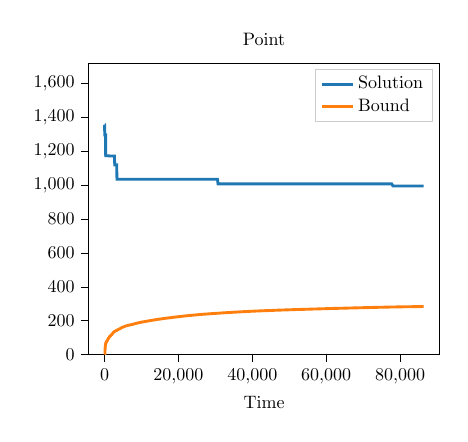
\begin{tikzpicture}[scale=0.65]

\definecolor{color0}{rgb}{0.12156862745098,0.466666666666667,0.705882352941177}
\definecolor{color1}{rgb}{1,0.498039215686275,0.0549019607843137}

\begin{axis}[
legend cell align={left},
legend style={fill opacity=0.8, draw opacity=1, text opacity=1, draw=white!80!black},
tick align=outside,
tick pos=left,
title={Point},
x grid style={white!69.0196078431373!black},
xlabel={Time},
xmin=-4307.6115, xmax=90668.044,
xtick style={color=black},
xtick={0, 20000, 40000, 60000, 80000},
scaled x ticks=false,
y grid style={white!69.0196078431373!black},
ymin=0,  ymax=1719.444425,
ytick style={color=black},
ytick={0, 200, ..., 1600},
scaled y ticks = false,
]
\addplot [ultra thick, color0]
table {%
11.8 1355.5956
14.42 1355.5956
22.86 1355.5956
31.41 1295.8849
39.63 1295.8849
49.85 1295.8849
59.61 1295.8849
68.38 1295.8849
76.52 1295.8849
84.82 1295.8849
95.31 1295.8849
127.03 1295.8849
161.71 1295.8849
196.19 1295.8849
230.97 1295.8849
266.42 1295.8849
299.44 1172.8275
338.56 1172.8275
371.74 1172.8275
405.64 1172.8275
444.93 1172.8275
479.18 1172.8275
518.23 1172.8275
555.24 1172.8275
590.72 1172.8275
626.21 1172.8275
661.29 1172.8275
696.37 1172.8275
731.15 1172.8275
769.34 1172.8275
808.77 1172.8275
843.51 1172.8275
879.9 1172.8275
914.16 1172.8275
955.44 1172.8275
990.83 1172.8275
1026.78 1172.8275
1066.47 1172.8275
1102.76 1172.8275
1140.56 1171.2427
1177.33 1171.2427
1211.66 1171.2427
1247.61 1171.2427
1284.19 1171.2427
1321.05 1171.2427
1357.9 1171.2427
1394.79 1171.2427
1433.2 1171.2427
1469.53 1171.2427
1505.89 1171.2427
1543.11 1171.2427
1584.55 1171.2427
1619.73 1171.2427
1656.1 1171.2427
1693.19 1171.2427
1729.58 1171.2427
1767.4 1171.2427
1802.87 1171.2427
1840.32 1171.2427
1880.81 1171.2427
1928.18 1171.2427
1965.81 1171.2427
2006.53 1171.2427
2043.9 1171.2427
2082.29 1171.2427
2119.38 1171.2427
2156.89 1171.2427
2194.65 1171.2427
2231.65 1171.2427
2270 1171.2427
2307.18 1171.2427
2347.19 1171.2427
2385.23 1171.2427
2424.01 1171.2427
2460.7 1171.2427
2502.38 1171.2427
2538.45 1171.2427
2573.77 1171.2427
2611.84 1171.2427
2656.94 1171.2427
2695.39 1136.4292
2736.45 1136.4292
2776.17 1119.1147
2814.49 1119.1147
2854.05 1119.1147
2893.92 1119.1147
2936.34 1119.1147
2974.81 1119.1147
3014.05 1119.1147
3052.65 1119.1147
3090.23 1119.1147
3126.94 1119.1147
3164.3 1119.1147
3202.72 1119.1147
3241.96 1119.1147
3281.45 1119.1147
3318.01 1066.0332
3356.37 1034.2717
3394.49 1034.2717
3433.98 1034.2717
3483.66 1034.2717
3637.69 1034.2717
3791.25 1034.2717
3947.49 1034.2717
4104.68 1034.2717
4254.6 1034.2717
4411.98 1034.2717
4560.27 1034.2717
4730.41 1034.2717
4882.46 1034.2717
5038.24 1034.2717
5207.34 1034.2717
5355.95 1034.2717
5508.94 1034.2717
5664.73 1034.2717
5820.74 1034.2717
5976.26 1034.2717
6129.91 1034.2717
6277.13 1034.2717
6430.33 1034.2717
6585.21 1034.2717
6735.83 1034.2717
6886.89 1034.2717
7038.03 1034.2717
7197.97 1034.2717
7347.65 1034.2717
7505.26 1034.2717
7657.17 1034.2717
7807.64 1034.2717
7956.97 1034.2717
8108.25 1034.2717
8258.69 1034.2717
8409.25 1034.2717
8557.64 1034.2717
8711.02 1034.2717
8873.57 1034.2717
9022.79 1034.2717
9171.03 1034.2717
9318.73 1034.2717
9466.08 1034.2717
9620.82 1034.2717
9767.35 1034.2717
9919.68 1034.2717
10073.53 1034.2717
10223.18 1034.2717
10402.73 1034.2717
10567.14 1034.2717
10733.3 1034.2717
10893.57 1034.2717
11051.22 1034.2717
11207.86 1034.2717
11369.9 1034.2717
11527.49 1034.2717
11686.93 1034.2717
11839.43 1034.2717
12001.86 1034.2717
12156.82 1034.2717
12312.08 1034.2717
12475.4 1034.2717
12630.95 1034.2717
12793.26 1034.2717
12944.47 1034.2717
13109.23 1034.2717
13273.66 1034.2717
13435.88 1034.2717
13588.21 1034.2717
13746.16 1034.2717
13903.01 1034.2717
14064.16 1034.2717
14224.99 1034.2717
14387.16 1034.2717
14548.33 1034.2717
14709.69 1034.2717
14880.11 1034.2717
15039.9 1034.2717
15193.6 1034.2717
15346.9 1034.2717
15505.6 1034.2717
15667.56 1034.2717
15839.18 1034.2717
16007.01 1034.2717
16171.56 1034.2717
16334.31 1034.2717
16495.19 1034.2717
16664.29 1034.2717
16825.92 1034.2717
16986.44 1034.2717
17147.89 1034.2717
17306.83 1034.2717
17469.43 1034.2717
17627.08 1034.2717
17780.82 1034.2717
17948.39 1034.2717
18108.99 1034.2717
18272.7 1034.2717
18431.93 1034.2717
18587.48 1034.2717
18751.7 1034.2717
18908.75 1034.2717
19057.19 1034.2717
19217.06 1034.2717
19378.77 1034.2717
19538.43 1034.2717
19702.93 1034.2717
19875.32 1034.2717
20037.98 1034.2717
20199.34 1034.2717
20387.65 1034.2717
20569.58 1034.2717
20753.36 1034.2717
20908.2 1034.2717
21066.04 1034.2717
21233.8 1034.2717
21400.64 1034.2717
21563.72 1034.2717
21720.98 1034.2717
21882.98 1034.2717
22039.83 1034.2717
22196.79 1034.2717
22356.42 1034.2717
22508.57 1034.2717
22656.14 1034.2717
22843.34 1034.2717
23007.98 1034.2717
23174.26 1034.2717
23337.5 1034.2717
23495.02 1034.2717
23659.89 1034.2717
23821.03 1034.2717
23989.66 1034.2717
24157.69 1034.2717
24322.92 1034.2717
24487.21 1034.2717
24653.66 1034.2717
24818.01 1034.2717
24978.67 1034.2717
25144.17 1034.2717
25316.87 1034.2717
25490.79 1034.2717
25642.18 1034.2717
25791.64 1034.2717
25949.51 1034.2717
26110.49 1034.2717
26273.49 1034.2717
26442.26 1034.2717
26593.03 1034.2717
26742 1034.2717
26892.89 1034.2717
27077.71 1034.2717
27244.77 1034.2717
27408.72 1034.2717
27573.81 1034.2717
27742.34 1034.2717
27902.34 1034.2717
28051.02 1034.2717
28211.35 1034.2717
28378.97 1034.2717
28558.72 1034.2717
28702.98 1034.2717
28877.82 1034.2717
29039.76 1034.2717
29210.83 1034.2717
29381.35 1034.2717
29545.94 1034.2717
29715.97 1034.2717
29877.26 1034.2717
30046.92 1034.2717
30213.2 1034.2717
30379.53 1034.2717
30550.7 1034.2717
30728.92 1006.6439
30916.79 1006.6439
31092.37 1006.6439
31263.54 1006.6439
31432.17 1006.6439
31597.35 1006.6439
31767.08 1006.6439
31939.07 1006.6439
32111.74 1006.6439
32301.54 1006.6439
32468.67 1006.6439
32643.78 1006.6439
32808.12 1006.6439
32973.38 1006.6439
33148.56 1006.6439
33308.54 1006.6439
33483.67 1006.6439
33647.74 1006.6439
33816.7 1006.6439
34014.65 1006.6439
34186.35 1006.6439
34365.49 1006.6439
34532.21 1006.6439
34702.94 1006.6439
34873.93 1006.6439
35035.5 1006.6439
35191.61 1006.6439
35349.78 1006.6439
35512.05 1006.6439
35681.13 1006.6439
35847.59 1006.6439
36019.71 1006.6439
36175.6 1006.6439
36340.75 1006.6439
36512.43 1006.6439
36716.22 1006.6439
36883.06 1006.6439
37040.55 1006.6439
37214.17 1006.6439
37377.49 1006.6439
37540.66 1006.6439
37705.85 1006.6439
37873.42 1006.6439
38037.31 1006.6439
38201.1 1006.6439
38366.92 1006.6439
38522.77 1006.6439
38672.92 1006.6439
38840.04 1006.6439
39007.57 1006.6439
39176.67 1006.6439
39330.52 1006.6439
39496.42 1006.6439
39661.06 1006.6439
39827.82 1006.6439
39988.48 1006.6439
40150.56 1006.6439
40318.77 1006.6439
40495.18 1006.6439
40662.47 1006.6439
40819.48 1006.6439
40987.29 1006.6439
41148.21 1006.6439
41315.43 1006.6439
41479.51 1006.6439
41651.87 1006.6439
41819.88 1006.6439
41976.74 1006.6439
42139.96 1006.6439
42299.46 1006.6439
42479.06 1006.6439
42659.98 1006.6439
42829.59 1006.6439
43028.21 1006.6439
43229.7 1006.6439
43420.45 1006.6439
43588.63 1006.6439
43770.34 1006.6439
43962.36 1006.6439
44161.24 1006.6439
44361.71 1006.6439
44511.27 1006.6439
44663.44 1006.6439
44834.07 1006.6439
45004.77 1006.6439
45157.03 1006.6439
45313.42 1006.6439
45468.14 1006.6439
45619.98 1006.6439
45777.28 1006.6439
45941.17 1006.6439
46098.06 1006.6439
46255.95 1006.6439
46428.31 1006.6439
46596.81 1006.6439
46760.47 1006.6439
46917.69 1006.6439
47080.39 1006.6439
47261.87 1006.6439
47450.15 1006.6439
47645.45 1006.6439
47839.11 1006.6439
48009.19 1006.6439
48178.66 1006.6439
48376.13 1006.6439
48567.41 1006.6439
48742.99 1006.6439
48927.16 1006.6439
49111.08 1006.6439
49298.19 1006.6439
49500.17 1006.6439
49651.15 1006.6439
49799.9 1006.6439
49949.12 1006.6439
50103.28 1006.6439
50260.01 1006.6439
50420.02 1006.6439
50571.75 1006.6439
50729.97 1006.6439
50885.69 1006.6439
51043.87 1006.6439
51201.28 1006.6439
51371.42 1006.6439
51552.06 1006.6439
51731.36 1006.6439
51924.95 1006.6439
52118.22 1006.6439
52303.16 1006.6439
52487.67 1006.6439
52682.55 1006.6439
52875.13 1006.6439
53065.32 1006.6439
53254.23 1006.6439
53445.84 1006.6439
53633.04 1006.6439
53823.22 1006.6439
54026.43 1006.6439
54216.87 1006.6439
54418.73 1006.6439
54595.81 1006.6439
54785.26 1006.6439
54980.79 1006.6439
55134.1 1006.6439
55286.45 1006.6439
55453.29 1006.6439
55623.58 1006.6439
55791.68 1006.6439
55963.2 1006.6439
56140.75 1006.6439
56310.88 1006.6439
56457.64 1006.6439
56632.26 1006.6439
56823.84 1006.6439
56987.06 1006.6439
57149.18 1006.6439
57318.31 1006.6439
57483.71 1006.6439
57644.73 1006.6439
57800.8 1006.6439
57962.59 1006.6439
58126.48 1006.6439
58287.47 1006.6439
58440.97 1006.6439
58596.97 1006.6439
58768.07 1006.6439
58949.57 1006.6439
59114.5 1006.6439
59261.43 1006.6439
59402.38 1006.6439
59560.49 1006.6439
59720.62 1006.6439
59874.39 1006.6439
60017.43 1006.6439
60164.15 1006.6439
60308.23 1006.6439
60447.07 1006.6439
60598 1006.6439
60765.9 1006.6439
60947.61 1006.6439
61144.84 1006.6439
61303.86 1006.6439
61465.62 1006.6439
61615.23 1006.6439
61771.92 1006.6439
61933.02 1006.6439
62112.15 1006.6439
62271.37 1006.6439
62431.59 1006.6439
62617.1 1006.6439
62802.77 1006.6439
62998.07 1006.6439
63185.59 1006.6439
63371.75 1006.6439
63534.62 1006.6439
63712.96 1006.6439
63887.94 1006.6439
64056.37 1006.6439
64216.05 1006.6439
64377.87 1006.6439
64539.99 1006.6439
64706.55 1006.6439
64877.18 1006.6439
65052.56 1006.6439
65236.6 1006.6439
65403.09 1006.6439
65566.84 1006.6439
65734.93 1006.6439
65905.87 1006.6439
66067.75 1006.6439
66229.69 1006.6439
66396.88 1006.6439
66555.03 1006.6439
66738.94 1006.6439
66890.48 1006.6439
67057.44 1006.6439
67224.27 1006.6439
67399.43 1006.6439
67579.32 1006.6439
67738.38 1006.6439
67903.9 1006.6439
68070.98 1006.6439
68261.71 1006.6439
68431.17 1006.6439
68600.06 1006.6439
68763.25 1006.6439
68956.78 1006.6439
69118.46 1006.6439
69273.04 1006.6439
69434.11 1006.6439
69598.58 1006.6439
69778.74 1006.6439
69930.21 1006.6439
70082.4 1006.6439
70230.67 1006.6439
70423.14 1006.6439
70579.58 1006.6439
70734.71 1006.6439
70884.76 1006.6439
71071.92 1006.6439
71247.31 1006.6439
71415.05 1006.6439
71581.06 1006.6439
71728.1 1006.6439
71911.35 1006.6439
72062.11 1006.6439
72214.78 1006.6439
72364.1 1006.6439
72524.91 1006.6439
72692.2 1006.6439
72839.41 1006.6439
72986.69 1006.6439
73142.67 1006.6439
73319.21 1006.6439
73466.25 1006.6439
73620.68 1006.6439
73791.31 1006.6439
73965.9 1006.6439
74140.26 1006.6439
74303.29 1006.6439
74462.66 1006.6439
74619.77 1006.6439
74811.59 1006.6439
74985.22 1006.6439
75150.73 1006.6439
75318.15 1006.6439
75500.64 1006.6439
75660.95 1006.6439
75810.59 1006.6439
75959.19 1006.6439
76115.57 1006.6439
76285.39 1006.6439
76445.39 1006.6439
76598.97 1006.6439
76754.38 1006.6439
76909.23 1006.6439
77097.95 1006.6439
77257.28 1006.6439
77415.87 1006.6439
77574.25 1006.6439
77751.49 1006.6439
77919.46 1000.3994
78085.25 994.1482
78242.21 994.1482
78409.42 994.1482
78585.34 994.1482
78755.79 994.1482
78916.83 994.1482
79077.4 994.1482
79244.82 994.1482
79423.39 994.1482
79596.42 994.1482
79767.18 994.1482
79945.21 994.1482
80122.48 994.1482
80275.3 994.1482
80440.76 994.1482
80607.66 994.1482
80781.54 994.1482
80948.05 994.1482
81143.23 994.1482
81318.4 994.1482
81530.33 994.1482
81741.03 994.1482
81937.54 994.1482
82124.51 994.1482
82332.62 994.1482
82552.29 994.1482
82772.51 994.1482
82979.35 994.1482
83158.34 994.1482
83329.25 994.1482
83498.39 994.1482
83662.58 994.1482
83825.19 994.1482
83995.65 994.1482
84174.46 994.1482
84335.82 994.1482
84515 994.1482
84696.13 994.1482
84866.75 994.1482
85036.4 994.1482
85207.33 994.1482
85371.6 994.1482
85538.25 994.1482
85741.15 994.1482
85941.1 994.1482
86144.35 994.1482
86351.08 994.1482
};
\addlegendentry{Solution}
\addplot [ultra thick, color1]
table {%
11.8 0
14.42 0
22.86 0
31.41 0
39.63 0
49.85 0
59.61 0
68.38 0
76.52 0
84.82 0
95.31 0
127.03 27.4958
161.71 40.1661
196.19 48.6544
230.97 54.4787
266.42 59.0156
299.44 65.8442
338.56 65.8442
371.74 68.0705
405.64 69.9943
444.93 72.6452
479.18 72.6452
518.23 75.4529
555.24 77.4169
590.72 78.8569
626.21 79.3824
661.29 80.6024
696.37 80.7026
731.15 82.5787
769.34 84.4552
808.77 86.0645
843.51 87.8538
879.9 88.7785
914.16 90.0476
955.44 91.8681
990.83 93.2549
1026.78 93.7869
1066.47 96.5203
1102.76 97.7329
1140.56 98.8022
1177.33 99.3027
1211.66 99.8392
1247.61 101.1446
1284.19 102.7638
1321.05 104.563
1357.9 104.7513
1394.79 105.9156
1433.2 106.939
1469.53 107.4144
1505.89 108.6038
1543.11 109.3027
1584.55 109.8858
1619.73 110.8492
1656.1 111.577
1693.19 113.2387
1729.58 114.3359
1767.4 115.2631
1802.87 116.0831
1840.32 116.76
1880.81 117.1692
1928.18 117.4745
1965.81 118.0534
2006.53 119.0591
2043.9 120.0068
2082.29 121.2698
2119.38 122.9861
2156.89 123.6441
2194.65 124.3621
2231.65 125.7179
2270 126.8119
2307.18 127.5658
2347.19 128.5491
2385.23 129.8714
2424.01 131.3917
2460.7 131.8158
2502.38 132.4031
2538.45 133.3437
2573.77 134.0831
2611.84 134.33
2656.94 135.2296
2695.39 135.6324
2736.45 136.1008
2776.17 136.5956
2814.49 137.0459
2854.05 137.5984
2893.92 138.1337
2936.34 138.6498
2974.81 139.0713
3014.05 139.463
3052.65 139.9104
3090.23 140.4141
3126.94 140.7299
3164.3 141.218
3202.72 141.7315
3241.96 142.3049
3281.45 142.7746
3318.01 142.9959
3356.37 143.259
3394.49 143.4276
3433.98 144.3968
3483.66 145.0799
3637.69 146.953
3791.25 148.4413
3947.49 150.3886
4104.68 151.8306
4254.6 153.3228
4411.98 155.4888
4560.27 157.7613
4730.41 159.7171
4882.46 161.0948
5038.24 162.52
5207.34 163.6436
5355.95 164.823
5508.94 166.468
5664.73 167.4229
5820.74 168.5687
5976.26 169.5985
6129.91 170.8299
6277.13 171.6175
6430.33 172.4116
6585.21 173.1459
6735.83 173.899
6886.89 174.7009
7038.03 175.2672
7197.97 176.0734
7347.65 176.8377
7505.26 177.3612
7657.17 178.2361
7807.64 179.2227
7956.97 180.2843
8108.25 181.3373
8258.69 181.9259
8409.25 182.7987
8557.64 183.7999
8711.02 184.7561
8873.57 185.6184
9022.79 186.4779
9171.03 186.7319
9318.73 187.8591
9466.08 188.5616
9620.82 189.0514
9767.35 189.738
9919.68 190.4783
10073.53 191.2491
10223.18 192.1463
10402.73 192.6183
10567.14 193.1708
10733.3 193.5816
10893.57 194.251
11051.22 194.9629
11207.86 195.639
11369.9 196.3101
11527.49 196.8759
11686.93 197.4871
11839.43 198.1431
12001.86 198.6534
12156.82 199.2413
12312.08 199.9135
12475.4 200.3555
12630.95 201.1338
12793.26 201.5819
12944.47 202.1111
13109.23 202.8083
13273.66 203.3539
13435.88 203.8951
13588.21 204.4412
13746.16 205.1735
13903.01 205.7284
14064.16 206.2686
14224.99 206.8818
14387.16 207.3886
14548.33 207.8219
14709.69 208.2179
14880.11 208.7507
15039.9 209.111
15193.6 209.542
15346.9 210.1687
15505.6 210.7689
15667.56 211.4113
15839.18 211.7148
16007.01 212.1758
16171.56 212.7072
16334.31 213.2444
16495.19 213.7893
16664.29 214.3659
16825.92 214.7792
16986.44 215.0796
17147.89 215.5603
17306.83 215.9973
17469.43 216.3331
17627.08 216.6858
17780.82 217.0038
17948.39 217.5467
18108.99 218.1681
18272.7 218.7966
18431.93 219.1684
18587.48 219.5027
18751.7 220.1597
18908.75 220.5082
19057.19 220.8854
19217.06 221.104
19378.77 221.4619
19538.43 221.8224
19702.93 222.2495
19875.32 222.7577
20037.98 223.1958
20199.34 223.5464
20387.65 223.9414
20569.58 224.3694
20753.36 224.8278
20908.2 225.3197
21066.04 225.7356
21233.8 226.1899
21400.64 226.5967
21563.72 227.1364
21720.98 227.5296
21882.98 227.7494
22039.83 228.1882
22196.79 228.5319
22356.42 228.8712
22508.57 229.163
22656.14 229.4236
22843.34 229.7083
23007.98 230.1042
23174.26 230.4449
23337.5 230.8795
23495.02 231.1771
23659.89 231.5015
23821.03 231.8612
23989.66 232.2735
24157.69 232.6387
24322.92 232.9163
24487.21 233.2851
24653.66 233.5306
24818.01 233.8499
24978.67 234.1818
25144.17 234.5572
25316.87 234.91
25490.79 235.2978
25642.18 235.6739
25791.64 235.9618
25949.51 236.2135
26110.49 236.5389
26273.49 236.7213
26442.26 237.041
26593.03 237.3206
26742 237.5743
26892.89 237.8695
27077.71 238.1849
27244.77 238.4011
27408.72 238.5836
27573.81 238.9363
27742.34 239.1473
27902.34 239.3853
28051.02 239.6287
28211.35 239.8383
28378.97 240.1367
28558.72 240.38
28702.98 240.6842
28877.82 240.965
29039.76 241.251
29210.83 241.5121
29381.35 241.7338
29545.94 241.9593
29715.97 242.2073
29877.26 242.4932
30046.92 242.7295
30213.2 243.0015
30379.53 243.1872
30550.7 243.4316
30728.92 243.6309
30916.79 243.8587
31092.37 244.0685
31263.54 244.41
31432.17 244.7644
31597.35 245.0419
31767.08 245.3068
31939.07 245.4272
32111.74 245.7413
32301.54 245.9988
32468.67 246.2252
32643.78 246.4332
32808.12 246.6389
32973.38 246.8502
33148.56 247.0045
33308.54 247.2642
33483.67 247.4989
33647.74 247.752
33816.7 247.9372
34014.65 248.1424
34186.35 248.4093
34365.49 248.6649
34532.21 248.8987
34702.94 249.0871
34873.93 249.3135
35035.5 249.6006
35191.61 249.8635
35349.78 250.0677
35512.05 250.2326
35681.13 250.3846
35847.59 250.607
36019.71 250.7875
36175.6 251.0193
36340.75 251.2025
36512.43 251.3828
36716.22 251.6414
36883.06 251.8952
37040.55 252.0762
37214.17 252.296
37377.49 252.4678
37540.66 252.6556
37705.85 252.8457
37873.42 253.1147
38037.31 253.348
38201.1 253.5073
38366.92 253.6816
38522.77 253.851
38672.92 254.0181
38840.04 254.1762
39007.57 254.385
39176.67 254.5691
39330.52 254.7515
39496.42 254.8711
39661.06 255.0715
39827.82 255.248
39988.48 255.3796
40150.56 255.5338
40318.77 255.7454
40495.18 255.8868
40662.47 256.0686
40819.48 256.2231
40987.29 256.4429
41148.21 256.5486
41315.43 256.7375
41479.51 256.9399
41651.87 257.0416
41819.88 257.2188
41976.74 257.3547
42139.96 257.4854
42299.46 257.6892
42479.06 257.7924
42659.98 257.98
42829.59 258.1138
43028.21 258.2896
43229.7 258.4429
43420.45 258.6216
43588.63 258.7346
43770.34 258.9366
43962.36 259.0692
44161.24 259.1767
44361.71 259.2961
44511.27 259.4018
44663.44 259.5381
44834.07 259.6437
45004.77 259.8269
45157.03 259.9298
45313.42 260.0889
45468.14 260.2618
45619.98 260.4881
45777.28 260.6184
45941.17 260.7713
46098.06 260.8877
46255.95 261.0434
46428.31 261.1668
46596.81 261.3085
46760.47 261.5042
46917.69 261.6046
47080.39 261.7589
47261.87 261.9133
47450.15 262.0363
47645.45 262.1671
47839.11 262.3286
48009.19 262.4228
48178.66 262.5029
48376.13 262.7
48567.41 262.8041
48742.99 262.9841
48927.16 263.0551
49111.08 263.2531
49298.19 263.3618
49500.17 263.5037
49651.15 263.6081
49799.9 263.724
49949.12 263.8663
50103.28 263.9841
50260.01 264.1326
50420.02 264.225
50571.75 264.3562
50729.97 264.4479
50885.69 264.5992
51043.87 264.7399
51201.28 264.8754
51371.42 265.0072
51552.06 265.1471
51731.36 265.2264
51924.95 265.3351
52118.22 265.4413
52303.16 265.5574
52487.67 265.7115
52682.55 265.8139
52875.13 265.9458
53065.32 266.0866
53254.23 266.1887
53445.84 266.2964
53633.04 266.379
53823.22 266.4922
54026.43 266.6099
54216.87 266.755
54418.73 266.8088
54595.81 266.9481
54785.26 267.0565
54980.79 267.1515
55134.1 267.2865
55286.45 267.3779
55453.29 267.5112
55623.58 267.6369
55791.68 267.8292
55963.2 267.9483
56140.75 268.0596
56310.88 268.1944
56457.64 268.2881
56632.26 268.3901
56823.84 268.4979
56987.06 268.5947
57149.18 268.7041
57318.31 268.787
57483.71 268.9095
57644.73 269.0078
57800.8 269.1016
57962.59 269.1988
58126.48 269.311
58287.47 269.4282
58440.97 269.5116
58596.97 269.6272
58768.07 269.7328
58949.57 269.8577
59114.5 269.9699
59261.43 270.0574
59402.38 270.1759
59560.49 270.2698
59720.62 270.3727
59874.39 270.4663
60017.43 270.5541
60164.15 270.6666
60308.23 270.7635
60447.07 270.8839
60598 270.978
60765.9 271.0497
60947.61 271.1869
61144.84 271.3037
61303.86 271.407
61465.62 271.4922
61615.23 271.5636
61771.92 271.725
61933.02 271.8167
62112.15 271.9208
62271.37 272.0202
62431.59 272.1304
62617.1 272.2344
62802.77 272.3272
62998.07 272.3991
63185.59 272.5159
63371.75 272.6033
63534.62 272.6652
63712.96 272.7386
63887.94 272.8551
64056.37 272.9571
64216.05 273.0329
64377.87 273.1205
64539.99 273.2361
64706.55 273.3413
64877.18 273.4555
65052.56 273.6035
65236.6 273.6652
65403.09 273.7535
65566.84 273.8325
65734.93 273.8998
65905.87 273.9907
66067.75 274.0857
66229.69 274.2197
66396.88 274.3147
66555.03 274.4545
66738.94 274.5663
66890.48 274.6556
67057.44 274.7477
67224.27 274.8439
67399.43 274.942
67579.32 275.0407
67738.38 275.1151
67903.9 275.1856
68070.98 275.259
68261.71 275.3367
68431.17 275.4283
68600.06 275.5285
68763.25 275.6186
68956.78 275.6943
69118.46 275.769
69273.04 275.8564
69434.11 275.9514
69598.58 276.0614
69778.74 276.1374
69930.21 276.1964
70082.4 276.3052
70230.67 276.3771
70423.14 276.4431
70579.58 276.5037
70734.71 276.6085
70884.76 276.7244
71071.92 276.8131
71247.31 276.8946
71415.05 276.9829
71581.06 277.0529
71728.1 277.1666
71911.35 277.2502
72062.11 277.3582
72214.78 277.4424
72364.1 277.5551
72524.91 277.6109
72692.2 277.7165
72839.41 277.8187
72986.69 277.9336
73142.67 278.0123
73319.21 278.0712
73466.25 278.1658
73620.68 278.2484
73791.31 278.332
73965.9 278.4308
74140.26 278.5126
74303.29 278.5865
74462.66 278.6738
74619.77 278.7648
74811.59 278.8567
74985.22 278.9503
75150.73 279.026
75318.15 279.1248
75500.64 279.1854
75660.95 279.2322
75810.59 279.338
75959.19 279.416
76115.57 279.4715
76285.39 279.5591
76445.39 279.6375
76598.97 279.7389
76754.38 279.791
76909.23 279.8505
77097.95 279.9393
77257.28 280.0046
77415.87 280.0825
77574.25 280.16
77751.49 280.2202
77919.46 280.3006
78085.25 280.3748
78242.21 280.4119
78409.42 280.4638
78585.34 280.5308
78755.79 280.603
78916.83 280.6955
79077.4 280.7628
79244.82 280.8309
79423.39 280.9084
79596.42 281.0013
79767.18 281.0706
79945.21 281.1364
80122.48 281.2059
80275.3 281.2511
80440.76 281.3275
80607.66 281.3724
80781.54 281.4357
80948.05 281.489
81143.23 281.5427
81318.4 281.5919
81530.33 281.6427
81741.03 281.7232
81937.54 281.7849
82124.51 281.851
82332.62 281.8963
82552.29 281.9671
82772.51 282.0166
82979.35 282.0723
83158.34 282.136
83329.25 282.2018
83498.39 282.299
83662.58 282.3432
83825.19 282.3902
83995.65 282.4555
84174.46 282.5086
84335.82 282.5602
84515 282.5949
84696.13 282.6479
84866.75 282.7092
85036.4 282.7691
85207.33 282.8432
85371.6 282.9162
85538.25 282.9611
85741.15 283.02
85941.1 283.1023
86144.35 283.2005
86351.08 283.2524
};
\addlegendentry{Bound}
\end{axis}

\end{tikzpicture}
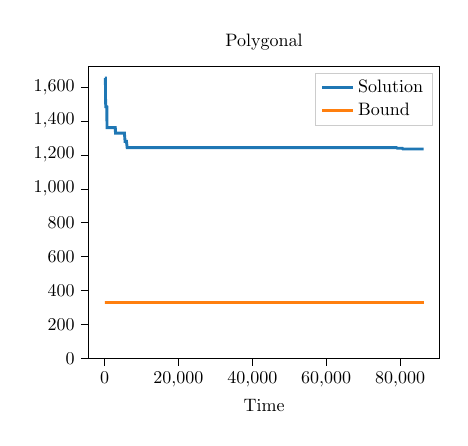
\begin{tikzpicture}[scale=0.65]

\definecolor{color0}{rgb}{0.12156862745098,0.466666666666667,0.705882352941177}
\definecolor{color1}{rgb}{1,0.498039215686275,0.0549019607843137}

\begin{axis}[
legend cell align={left},
legend style={fill opacity=0.8, draw opacity=1, text opacity=1, draw=white!80!black},
tick align=outside,
tick pos=left,
title={Polygonal},
x grid style={white!69.0196078431373!black},
xlabel={Time},
xmin=-4307.6115, xmax=90668.044,
xtick style={color=black},
xtick={0, 20000, 40000, 60000, 80000},
scaled x ticks=false,
y grid style={white!69.0196078431373!black},
ymin=0, ymax=1719.444425,
ytick style={color=black},
ytick={0, 200, ..., 1600},
scaled y ticks = false,
]
\addplot [ultra thick, color0]
table {%
74.57 1653.3316
93.74 1653.3316
109.8 1653.3316
120.56 1653.3316
131.35 1653.3316
139.06 1653.3316
152.7 1653.3316
164.09 1653.3316
171.46 1653.3316
182.73 1653.3316
192.44 1653.3316
221.85 1653.3316
252.6 1520.0428
279.86 1520.0428
310.38 1483.9327
340.76 1483.9327
372.7 1483.9327
403.61 1483.9327
433.52 1483.9327
465.69 1483.9327
499.19 1483.9327
535.14 1483.9327
568.79 1483.9327
604.12 1483.9327
642.45 1385.9091
680.07 1360.83
716.82 1360.83
756.22 1360.83
795.63 1360.83
833.99 1360.83
871.41 1360.83
916.46 1360.83
954.31 1360.83
989.12 1360.83
1023.24 1360.83
1059.21 1360.83
1096.7 1360.83
1138.91 1360.83
1181.9 1360.83
1224.1 1360.83
1260.64 1360.83
1297.44 1360.83
1340.24 1360.83
1384.61 1360.83
1434.69 1360.83
1474.52 1360.83
1516.59 1360.83
1560.64 1360.83
1602.65 1360.83
1646.03 1360.83
1686.81 1360.83
1726.61 1360.83
1765.45 1360.83
1809.92 1360.83
1855.88 1360.83
1904.55 1360.83
1954.08 1360.83
1995.92 1360.83
2041.32 1360.83
2082.12 1360.83
2123.78 1360.83
2169.9 1360.83
2213.48 1360.83
2254.13 1360.83
2302.64 1360.83
2350.37 1360.83
2405.67 1360.83
2458.89 1360.83
2509.3 1360.83
2553.56 1360.83
2598.32 1360.83
2636.78 1360.83
2682.47 1360.83
2724.68 1360.83
2766.96 1360.83
2810.35 1360.83
2861.35 1360.83
2900.4 1360.83
2948.31 1328.048
2991.63 1328.048
3042.49 1328.048
3085.73 1328.048
3139.95 1328.048
3186.29 1328.048
3236.99 1328.048
3281.33 1328.048
3319.97 1328.048
3361.69 1328.048
3400.17 1328.048
3447.48 1328.048
3493.26 1328.048
3542.63 1328.048
3581.03 1328.048
3618.06 1328.048
3661.96 1328.048
3704.1 1328.048
3744.83 1328.048
3796.28 1328.048
3840.52 1328.048
3885.84 1328.048
3939.52 1328.048
4097.14 1328.048
4291.94 1328.048
4469.15 1328.048
4652.73 1328.048
4818.51 1328.048
4988.17 1328.048
5176.55 1328.048
5370.65 1328.048
5546.23 1279.4325
5733.48 1279.4325
5922.03 1279.4325
6113.14 1242.5617
6315.29 1242.5617
6519.19 1242.5617
6725.85 1242.5617
6906.69 1242.5617
7087.49 1242.5617
7270.21 1242.5617
7438.23 1242.5617
7640.62 1242.5617
7807.86 1242.5617
7986.27 1242.5617
8163.27 1242.5617
8353.68 1242.5617
8539.34 1242.5617
8730.07 1242.5617
8897.77 1242.5617
9082.41 1242.5617
9264.67 1242.5617
9458.53 1242.5617
9649.62 1242.5617
9844.37 1242.5617
10043.52 1242.5617
10252.82 1242.5617
10476.3 1242.5617
10716.64 1242.5617
10926.37 1242.5617
11150.09 1242.5617
11367.07 1242.5617
11572.44 1242.5617
11801.25 1242.5617
12006.94 1242.5617
12219.29 1242.5617
12438.23 1242.5617
12644.8 1242.5617
12882.34 1242.5617
13128.43 1242.5617
13329.91 1242.5617
13545.32 1242.5617
13772.1 1242.5617
13994 1242.5617
14275.62 1242.5617
14465.05 1242.5617
14680.7 1242.5617
14887.53 1242.5617
15117.71 1242.5617
15320.75 1242.5617
15541.77 1242.5617
15798.18 1242.5617
16016.33 1242.5617
16258.06 1242.5617
16480.75 1242.5617
16697.1 1242.5617
16911.75 1242.5617
17161.78 1242.5617
17375.86 1242.5617
17576.9 1242.5617
17768.77 1242.5617
18004.5 1242.5617
18232.58 1242.5617
18464.11 1242.5617
18702.04 1242.5617
18987.31 1242.5617
19214.84 1242.5617
19457.24 1242.5617
19723.85 1242.5617
19902.04 1242.5617
20064.51 1242.5617
20264.99 1242.5617
20532.76 1242.5617
20761.59 1242.5617
20948.65 1242.5617
21114.61 1242.5617
21289.2 1242.5617
21486.91 1242.5617
21668.74 1242.5617
21915.07 1242.5617
22156.36 1242.5617
22359.83 1242.5617
22599.66 1242.5617
22856.13 1242.5617
23084.63 1242.5617
23330.19 1242.5617
23564.78 1242.5617
23729.72 1242.5617
23926.39 1242.5617
24135.04 1242.5617
24369.19 1242.5617
24614.17 1242.5617
24821.65 1242.5617
25041.35 1242.5617
25263.32 1242.5617
25480.51 1242.5617
25710.51 1242.5617
25947.28 1242.5617
26155.98 1242.5617
26399.78 1242.5617
26629.29 1242.5617
26833.7 1242.5617
27074.85 1242.5617
27277.06 1242.5617
27461.18 1242.5617
27727.88 1242.5617
27971.11 1242.5617
28203.34 1242.5617
28430.86 1242.5617
28628.3 1242.5617
28808.83 1242.5617
28973.29 1242.5617
29151.52 1242.5617
29348.99 1242.5617
29590.9 1242.5617
29788.43 1242.5617
29996.29 1242.5617
30221.03 1242.5617
30406.17 1242.5617
30602.28 1242.5617
30820.47 1242.5617
31039.24 1242.5617
31261.28 1242.5617
31464.23 1242.5617
31663.66 1242.5617
31847.83 1242.5617
32050.92 1242.5617
32251.15 1242.5617
32459.63 1242.5617
32662.95 1242.5617
32857.25 1242.5617
33042.1 1242.5617
33253.5 1242.5617
33441.29 1242.5617
33637.23 1242.5617
33842.59 1242.5617
34060.14 1242.5617
34265.41 1242.5617
34464.26 1242.5617
34670.28 1242.5617
34879.25 1242.5617
35115.17 1242.5617
35326.09 1242.5617
35538.63 1242.5617
35761.42 1242.5617
36002.25 1242.5617
36229.81 1242.5617
36430.17 1242.5617
36682.82 1242.5617
36937.03 1242.5617
37147.71 1242.5617
37350.84 1242.5617
37532.65 1242.5617
37751.09 1242.5617
37991.99 1242.5617
38188.42 1242.5617
38407.72 1242.5617
38619.31 1242.5617
38837.55 1242.5617
39060.29 1242.5617
39251.49 1242.5617
39468.84 1242.5617
39729.69 1242.5617
39908.6 1242.5617
40111.84 1242.5617
40290.42 1242.5617
40480.69 1242.5617
40684.93 1242.5617
40874.61 1242.5617
41033.61 1242.5617
41226.83 1242.5617
41425.32 1242.5617
41637.11 1242.5617
41825.08 1242.5617
42052.15 1242.5617
42256.94 1242.5617
42465.03 1242.5617
42680.95 1242.5617
42928.84 1242.5617
43161.44 1242.5617
43407.53 1242.5617
43633.95 1242.5617
43912.05 1242.5617
44182.61 1242.5617
44403.77 1242.5617
44628.39 1242.5617
44830.03 1242.5617
45028.67 1242.5617
45174.69 1242.5617
45415.93 1242.5617
45681.42 1242.5617
45929.58 1242.5617
46160.82 1242.5617
46398.24 1242.5617
46679.25 1242.5617
46897.98 1242.5617
47164.34 1242.5617
47420.93 1242.5617
47717.12 1242.5617
47962.22 1242.5617
48176.97 1242.5617
48398.28 1242.5617
48599.88 1242.5617
48842.72 1242.5617
49079.77 1242.5617
49276.71 1242.5617
49479.62 1242.5617
49636.6 1242.5617
49856.15 1242.5617
50086.72 1242.5617
50355.84 1242.5617
50594.73 1242.5617
50830.91 1242.5617
51083.53 1242.5617
51351.32 1242.5617
51586.17 1242.5617
51840.93 1242.5617
52116.16 1242.5617
52360.85 1242.5617
52564.34 1242.5617
52798.99 1242.5617
53053.9 1242.5617
53300.64 1242.5617
53547.78 1242.5617
53832.08 1242.5617
54086.13 1242.5617
54339.02 1242.5617
54618.76 1242.5617
54863.48 1242.5617
55130.31 1242.5617
55366.14 1242.5617
55633.66 1242.5617
55889.79 1242.5617
56123.57 1242.5617
56364.04 1242.5617
56599.85 1242.5617
56784.91 1242.5617
56971.1 1242.5617
57168.06 1242.5617
57362.71 1242.5617
57586.32 1242.5617
57758.57 1242.5617
57953.91 1242.5617
58156.83 1242.5617
58383.02 1242.5617
58619.36 1242.5617
58895.95 1242.5617
59220.99 1242.5617
59483.25 1242.5617
59751.64 1242.5617
59985.05 1242.5617
60224.32 1242.5617
60455.19 1242.5617
60641.45 1242.5617
60866.94 1242.5617
61159.43 1242.5617
61379.02 1242.5617
61606.62 1242.5617
61821.67 1242.5617
62034.36 1242.5617
62249.33 1242.5617
62488.3 1242.5617
62736.1 1242.5617
62996.44 1242.5617
63263.91 1242.5617
63492.22 1242.5617
63703.42 1242.5617
63934.28 1242.5617
64204.21 1242.5617
64440.99 1242.5617
64659.72 1242.5617
64883.57 1242.5617
65088 1242.5617
65299.34 1242.5617
65484.77 1242.5617
65672.88 1242.5617
65870.72 1242.5617
66066.88 1242.5617
66289.4 1242.5617
66502.38 1242.5617
66736.59 1242.5617
66966.25 1242.5617
67162.91 1242.5617
67370.74 1242.5617
67553.52 1242.5617
67758.87 1242.5617
67947.74 1242.5617
68152.71 1242.5617
68326.36 1242.5617
68526.11 1242.5617
68747.9 1242.5617
69004.06 1242.5617
69269.62 1242.5617
69480.74 1242.5617
69719.38 1242.5617
69949.99 1242.5617
70210.48 1242.5617
70462.68 1242.5617
70667.95 1242.5617
70928.41 1242.5617
71175.84 1242.5617
71397.04 1242.5617
71616.71 1242.5617
71880.52 1242.5617
72106.67 1242.5617
72347.03 1242.5617
72568.45 1242.5617
72794.69 1242.5617
73058.46 1242.5617
73269.54 1242.5617
73434.88 1242.5617
73634.74 1242.5617
73845.98 1242.5617
74075.98 1242.5617
74283.77 1242.5617
74502.05 1242.5617
74736.26 1242.5617
74985.91 1242.5617
75196.68 1242.5617
75395.03 1242.5617
75647.1 1242.5617
75880.87 1242.5617
76107.39 1242.5617
76342.28 1242.5617
76562.32 1242.5617
76791.38 1242.5617
77001.47 1242.5617
77197.29 1242.5617
77384.41 1242.5617
77591.64 1242.5617
77769.8 1242.5617
77949.45 1242.5617
78177.48 1242.5617
78360.22 1242.5607
78568.15 1242.5607
78797.01 1242.5607
79019.82 1242.5607
79245.04 1238.8348
79474.59 1238.8348
79669.94 1238.8348
79882.06 1238.8348
80096.19 1238.8049
80316.34 1238.8049
80602.69 1238.8049
80800.53 1234.4645
81064.14 1234.4645
81361.92 1234.4645
81666.38 1234.4645
81911.98 1234.4645
82200.04 1234.4645
82532.43 1234.4645
82870.06 1234.4645
83155.82 1234.4645
83393.15 1234.4645
83679.66 1234.4645
83928.43 1234.4645
84157.2 1234.4645
84407.72 1234.4645
84666.86 1234.4645
84971.78 1234.4645
85213.32 1234.4645
85442.91 1234.4645
85687.39 1234.4645
85962.01 1234.4645
86236.98 1234.4645
86400.03 1234.4645
};
\addlegendentry{Solution}
\addplot [ultra thick, color1]
table {%
74.57 331.0751
93.74 331.0751
109.8 331.0751
120.56 331.0751
131.35 331.0751
139.06 331.0751
152.7 331.0751
164.09 331.0751
171.46 331.0751
182.73 331.0751
192.44 331.0751
221.85 331.0751
252.6 331.0751
279.86 331.0751
310.38 331.0751
340.76 331.0751
372.7 331.0751
403.61 331.0751
433.52 331.0751
465.69 331.0751
499.19 331.0751
535.14 331.0751
568.79 331.0751
604.12 331.0751
642.45 331.0751
680.07 331.0751
716.82 331.0751
756.22 331.0751
795.63 331.0751
833.99 331.0751
871.41 331.0751
916.46 331.0751
954.31 331.0751
989.12 331.0751
1023.24 331.0751
1059.21 331.0751
1096.7 331.0751
1138.91 331.0751
1181.9 331.0751
1224.1 331.0751
1260.64 331.0751
1297.44 331.0751
1340.24 331.0751
1384.61 331.0751
1434.69 331.0751
1474.52 331.0751
1516.59 331.0751
1560.64 331.0751
1602.65 331.0751
1646.03 331.0751
1686.81 331.0751
1726.61 331.0751
1765.45 331.0751
1809.92 331.0751
1855.88 331.0751
1904.55 331.0751
1954.08 331.0751
1995.92 331.0751
2041.32 331.0751
2082.12 331.0751
2123.78 331.0751
2169.9 331.0751
2213.48 331.0751
2254.13 331.0751
2302.64 331.0751
2350.37 331.0751
2405.67 331.0751
2458.89 331.0751
2509.3 331.0751
2553.56 331.0751
2598.32 331.0751
2636.78 331.0751
2682.47 331.0751
2724.68 331.0751
2766.96 331.0751
2810.35 331.0751
2861.35 331.0751
2900.4 331.0751
2948.31 331.0751
2991.63 331.0751
3042.49 331.0751
3085.73 331.0751
3139.95 331.0751
3186.29 331.0751
3236.99 331.0751
3281.33 331.0751
3319.97 331.0751
3361.69 331.0751
3400.17 331.0751
3447.48 331.0751
3493.26 331.0751
3542.63 331.0751
3581.03 331.0751
3618.06 331.0751
3661.96 331.0751
3704.1 331.0751
3744.83 331.0751
3796.28 331.0751
3840.52 331.0751
3885.84 331.0751
3939.52 331.0751
4097.14 331.0751
4291.94 331.0751
4469.15 331.0751
4652.73 331.0751
4818.51 331.0751
4988.17 331.0751
5176.55 331.0751
5370.65 331.0751
5546.23 331.0751
5733.48 331.0751
5922.03 331.0751
6113.14 331.0751
6315.29 331.0751
6519.19 331.0751
6725.85 331.0751
6906.69 331.0751
7087.49 331.0751
7270.21 331.0751
7438.23 331.0751
7640.62 331.0751
7807.86 331.0751
7986.27 331.0751
8163.27 331.0751
8353.68 331.0751
8539.34 331.0751
8730.07 331.0751
8897.77 331.0751
9082.41 331.0751
9264.67 331.0751
9458.53 331.0751
9649.62 331.0751
9844.37 331.0751
10043.52 331.0751
10252.82 331.0751
10476.3 331.0751
10716.64 331.0751
10926.37 331.0751
11150.09 331.0751
11367.07 331.0751
11572.44 331.0751
11801.25 331.0751
12006.94 331.0751
12219.29 331.0751
12438.23 331.0751
12644.8 331.0751
12882.34 331.0751
13128.43 331.0751
13329.91 331.0751
13545.32 331.0751
13772.1 331.0751
13994 331.0751
14275.62 331.0751
14465.05 331.0751
14680.7 331.0751
14887.53 331.0751
15117.71 331.0751
15320.75 331.0751
15541.77 331.0751
15798.18 331.0751
16016.33 331.0751
16258.06 331.0751
16480.75 331.0751
16697.1 331.0751
16911.75 331.0751
17161.78 331.0751
17375.86 331.0751
17576.9 331.0751
17768.77 331.0751
18004.5 331.0751
18232.58 331.0751
18464.11 331.0751
18702.04 331.0751
18987.31 331.0751
19214.84 331.0751
19457.24 331.0751
19723.85 331.0751
19902.04 331.0751
20064.51 331.0751
20264.99 331.0751
20532.76 331.0751
20761.59 331.0751
20948.65 331.0751
21114.61 331.0751
21289.2 331.0751
21486.91 331.0751
21668.74 331.0751
21915.07 331.0751
22156.36 331.0751
22359.83 331.0751
22599.66 331.0751
22856.13 331.0751
23084.63 331.0751
23330.19 331.0751
23564.78 331.0751
23729.72 331.0751
23926.39 331.0751
24135.04 331.0751
24369.19 331.0751
24614.17 331.0751
24821.65 331.0751
25041.35 331.0751
25263.32 331.0751
25480.51 331.0751
25710.51 331.0751
25947.28 331.0751
26155.98 331.0751
26399.78 331.0751
26629.29 331.0751
26833.7 331.0751
27074.85 331.0751
27277.06 331.0751
27461.18 331.0751
27727.88 331.0751
27971.11 331.0751
28203.34 331.0751
28430.86 331.0751
28628.3 331.0751
28808.83 331.0751
28973.29 331.0751
29151.52 331.0751
29348.99 331.0751
29590.9 331.0751
29788.43 331.0751
29996.29 331.0751
30221.03 331.0751
30406.17 331.0751
30602.28 331.0751
30820.47 331.0751
31039.24 331.0751
31261.28 331.0751
31464.23 331.0751
31663.66 331.0751
31847.83 331.0751
32050.92 331.0751
32251.15 331.0751
32459.63 331.0751
32662.95 331.0751
32857.25 331.0751
33042.1 331.0751
33253.5 331.0751
33441.29 331.0751
33637.23 331.0751
33842.59 331.0751
34060.14 331.0751
34265.41 331.0751
34464.26 331.0751
34670.28 331.0751
34879.25 331.0751
35115.17 331.0751
35326.09 331.0751
35538.63 331.0751
35761.42 331.0751
36002.25 331.0751
36229.81 331.0751
36430.17 331.0751
36682.82 331.0751
36937.03 331.0751
37147.71 331.0751
37350.84 331.0751
37532.65 331.0751
37751.09 331.0751
37991.99 331.0751
38188.42 331.0751
38407.72 331.0751
38619.31 331.0751
38837.55 331.0751
39060.29 331.0751
39251.49 331.0751
39468.84 331.0751
39729.69 331.0751
39908.6 331.0751
40111.84 331.0751
40290.42 331.0751
40480.69 331.0751
40684.93 331.0751
40874.61 331.0751
41033.61 331.0751
41226.83 331.0751
41425.32 331.0751
41637.11 331.0751
41825.08 331.0751
42052.15 331.0751
42256.94 331.0751
42465.03 331.0751
42680.95 331.0751
42928.84 331.0751
43161.44 331.0751
43407.53 331.0751
43633.95 331.0751
43912.05 331.0751
44182.61 331.0751
44403.77 331.0751
44628.39 331.0751
44830.03 331.0751
45028.67 331.0751
45174.69 331.0751
45415.93 331.0751
45681.42 331.0751
45929.58 331.0751
46160.82 331.0751
46398.24 331.0751
46679.25 331.0751
46897.98 331.0751
47164.34 331.0751
47420.93 331.0751
47717.12 331.0751
47962.22 331.0751
48176.97 331.0751
48398.28 331.0751
48599.88 331.0751
48842.72 331.0751
49079.77 331.0751
49276.71 331.0751
49479.62 331.0751
49636.6 331.0751
49856.15 331.0751
50086.72 331.0751
50355.84 331.0751
50594.73 331.0751
50830.91 331.0751
51083.53 331.0751
51351.32 331.0751
51586.17 331.0751
51840.93 331.0751
52116.16 331.0751
52360.85 331.0751
52564.34 331.0751
52798.99 331.0751
53053.9 331.0751
53300.64 331.0751
53547.78 331.0751
53832.08 331.0751
54086.13 331.0751
54339.02 331.0751
54618.76 331.0751
54863.48 331.0751
55130.31 331.0751
55366.14 331.0751
55633.66 331.0751
55889.79 331.0751
56123.57 331.0751
56364.04 331.0751
56599.85 331.0751
56784.91 331.0751
56971.1 331.0751
57168.06 331.0751
57362.71 331.0751
57586.32 331.0751
57758.57 331.0751
57953.91 331.0751
58156.83 331.0751
58383.02 331.0751
58619.36 331.0751
58895.95 331.0751
59220.99 331.0751
59483.25 331.0751
59751.64 331.0751
59985.05 331.0751
60224.32 331.0751
60455.19 331.0751
60641.45 331.0751
60866.94 331.0751
61159.43 331.0751
61379.02 331.0751
61606.62 331.0751
61821.67 331.0751
62034.36 331.0751
62249.33 331.0751
62488.3 331.0751
62736.1 331.0751
62996.44 331.0751
63263.91 331.0751
63492.22 331.0751
63703.42 331.0751
63934.28 331.0751
64204.21 331.0751
64440.99 331.0751
64659.72 331.0751
64883.57 331.0751
65088 331.0751
65299.34 331.0751
65484.77 331.0751
65672.88 331.0751
65870.72 331.0751
66066.88 331.0751
66289.4 331.0751
66502.38 331.0751
66736.59 331.0751
66966.25 331.0751
67162.91 331.0751
67370.74 331.0751
67553.52 331.0751
67758.87 331.0751
67947.74 331.0751
68152.71 331.0751
68326.36 331.0751
68526.11 331.0751
68747.9 331.0751
69004.06 331.0751
69269.62 331.0751
69480.74 331.0751
69719.38 331.0751
69949.99 331.0751
70210.48 331.0751
70462.68 331.0751
70667.95 331.0751
70928.41 331.0751
71175.84 331.0751
71397.04 331.0751
71616.71 331.0751
71880.52 331.0751
72106.67 331.0751
72347.03 331.0751
72568.45 331.0751
72794.69 331.0751
73058.46 331.0751
73269.54 331.0751
73434.88 331.0751
73634.74 331.0751
73845.98 331.0751
74075.98 331.0751
74283.77 331.0751
74502.05 331.0751
74736.26 331.0751
74985.91 331.0751
75196.68 331.0751
75395.03 331.0751
75647.1 331.0751
75880.87 331.0751
76107.39 331.0751
76342.28 331.0751
76562.32 331.0751
76791.38 331.0751
77001.47 331.0751
77197.29 331.0751
77384.41 331.0751
77591.64 331.0751
77769.8 331.0751
77949.45 331.0751
78177.48 331.0751
78360.22 331.0751
78568.15 331.0751
78797.01 331.0751
79019.82 331.0751
79245.04 331.0751
79474.59 331.0751
79669.94 331.0751
79882.06 331.0751
80096.19 331.0751
80316.34 331.0751
80602.69 331.0751
80800.53 331.0751
81064.14 331.0751
81361.92 331.0751
81666.38 331.0751
81911.98 331.0751
82200.04 331.0751
82532.43 331.0751
82870.06 331.0751
83155.82 331.0751
83393.15 331.0751
83679.66 331.0751
83928.43 331.0751
84157.2 331.0751
84407.72 331.0751
84666.86 331.0751
84971.78 331.0751
85213.32 331.0751
85442.91 331.0751
85687.39 331.0751
85962.01 331.0751
86236.98 331.0751
86400.03 331.0751
};
\addlegendentry{Bound}
\end{axis}

\end{tikzpicture}
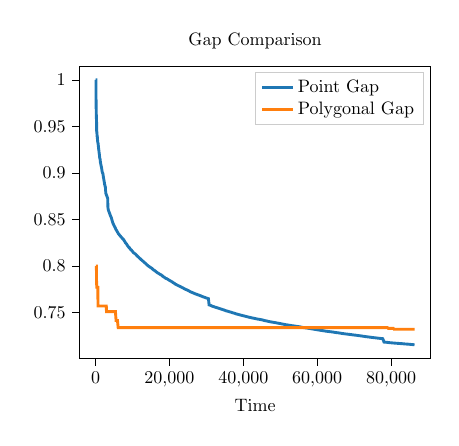
\begin{tikzpicture}[scale=0.65]

\definecolor{color0}{rgb}{0.12156862745098,0.466666666666667,0.705882352941177}
\definecolor{color1}{rgb}{1,0.498039215686275,0.0549019607843137}

\begin{axis}[
legend cell align={left},
legend style={fill opacity=0.8, draw opacity=1, text opacity=1, draw=white!80!black},
tick align=outside,
tick pos=left,
title={Gap Comparison},
x grid style={white!69.0196078431373!black},
xlabel={Time},
xmin=-4307.6115, xmax=90668.044,
xtick style={color=black},
xtick={0, 20000, 40000, 60000, 80000},
scaled x ticks=false,
y grid style={white!69.0196078431373!black},
ymin=0.70083432228716, ymax=1.01424598465299,
ytick style={color=black},
ytick={0.75, 0.8 , ..., 1.05},
scaled y ticks = false,
]
\addplot [ultra thick, color0]
table {%
11.8 1
14.42 1
22.86 1
31.41 1
39.63 1
49.85 1
59.61 1
68.38 1
76.52 1
84.82 1
95.31 1
127.03 0.978782220550606
161.71 0.969004886159257
196.19 0.962454690227504
230.97 0.957960232424963
266.42 0.95445922705018
299.44 0.943858581078633
338.56 0.943858581078633
371.74 0.941960347962509
405.64 0.940320038539342
444.93 0.938059774348743
479.18 0.938059774348743
518.23 0.93566581615796
555.24 0.93399123059444
590.72 0.93276342855194
626.21 0.932315366070458
661.29 0.931275144895562
696.37 0.931189710336772
731.15 0.929590071856262
769.34 0.927990092319629
808.77 0.926617938273105
843.51 0.925092308971268
879.9 0.924303872479116
914.16 0.923221786665132
955.44 0.921669554985708
990.83 0.920487113407556
1026.78 0.920033508764077
1066.47 0.917702901748126
1102.76 0.916668990111504
1140.56 0.915643273593082
1177.33 0.915215949691725
1211.66 0.914757889206054
1247.61 0.91364334650709
1284.19 0.912260883248194
1321.05 0.910724737067731
1357.9 0.910563967655892
1394.79 0.909569895291557
1433.2 0.908696122503047
1469.53 0.908290228831309
1505.89 0.907274726237355
1543.11 0.90667800960467
1584.55 0.906180162318194
1619.73 0.905357617170207
1656.1 0.904736225890671
1693.19 0.903317476386406
1729.58 0.902380693600054
1767.4 0.901589055795182
1802.87 0.900888944708044
1840.32 0.900311011543551
1880.81 0.899961639035189
1928.18 0.899700975724331
1965.81 0.899206714372692
2006.53 0.898348053738136
2043.9 0.897538913156086
2082.29 0.896460571323091
2119.38 0.89499520466595
2156.89 0.894433408208222
2194.65 0.893820384109971
2231.65 0.892662810192968
2270 0.891728759547445
2307.18 0.891085084244282
2347.19 0.890245548595522
2385.23 0.88911657677781
2424.01 0.887818553746376
2460.7 0.887456459707283
2502.38 0.886955026485971
2538.45 0.886151947841382
2573.77 0.885520652551346
2611.84 0.885309850810596
2656.94 0.884541777720365
2695.39 0.880650373996022
2736.45 0.88023820577648
2776.17 0.877943163466622
2814.49 0.87754079184198
2854.05 0.877047098032043
2893.92 0.876568773513564
2936.34 0.876107605413458
2974.81 0.875730968416374
3014.05 0.875380959610306
3052.65 0.874981179319689
3090.23 0.874531091406448
3126.94 0.874248904066759
3164.3 0.873812755743446
3202.72 0.873353910908328
3241.96 0.872841541622141
3281.45 0.872421834866435
3318.01 0.86586168235661
3356.37 0.861488040328281
3394.49 0.861325027069773
3433.98 0.860387942549332
3483.66 0.859727477799112
3637.69 0.857916444972825
3791.25 0.856477461386597
3947.49 0.854594687256743
4104.68 0.85320046947045
4254.6 0.851757715114897
4411.98 0.849663487843668
4560.27 0.847466289563951
4730.41 0.845575297090697
4882.46 0.844243248655068
5038.24 0.84286527418279
5207.34 0.841778905871639
5355.95 0.840638586553224
5508.94 0.839048095389248
5664.73 0.838124837022999
5820.74 0.837017004332614
5976.26 0.836021327858047
6129.91 0.8348307316153
6277.13 0.834069229584451
6430.33 0.83330144293806
6585.21 0.832591474754651
6735.83 0.831863329529368
6886.89 0.831088001344328
7038.03 0.83054046630107
7197.97 0.829760980601132
7347.65 0.829022006499839
7505.26 0.828515853232763
7657.17 0.827669943980871
7807.64 0.826716036028057
7956.97 0.825689613280533
8108.25 0.824671505562803
8258.69 0.824102409453918
8409.25 0.823258530616278
8557.64 0.822290506450094
8711.02 0.821365991160736
8873.57 0.820532264394356
9022.79 0.819701244846978
9171.03 0.819455661408893
9318.73 0.818365812387596
9466.08 0.817686590477144
9620.82 0.817213020524491
9767.35 0.816549171750518
9919.68 0.815833402383532
10073.53 0.815088143666698
10223.18 0.814220673349179
10402.73 0.81376431357447
10567.14 0.813230121253439
10733.3 0.812832933551213
10893.57 0.812185714836827
11051.22 0.811497404405438
11207.86 0.810843707702725
11369.9 0.810194845319658
11527.49 0.809647793708365
11686.93 0.809056846474674
11839.43 0.808422583736943
12001.86 0.807929193073735
12156.82 0.8073607737696
12312.08 0.806710847836212
12475.4 0.806283493979387
12630.95 0.805530983783081
12793.26 0.805097732056287
12944.47 0.804586067664812
13109.23 0.803911970133186
13273.66 0.803384449173268
13435.88 0.80286118241464
13588.21 0.802333178022757
13746.16 0.801625143567208
13903.01 0.801088630772746
14064.16 0.800566330878047
14224.99 0.799973449916497
14387.16 0.799483443277042
14548.33 0.799064501136403
14709.69 0.798681623020334
14880.11 0.798166477918713
15039.9 0.797818116844926
15193.6 0.797401398491325
15346.9 0.796795464866727
15505.6 0.79621515313626
15667.56 0.795594039747969
15839.18 0.795300596545376
16007.01 0.794854872273891
16171.56 0.794341080781771
16334.31 0.793821681478861
16495.19 0.793294837323694
16664.29 0.792737343581962
16825.92 0.792337738719913
16986.44 0.7920472927955
17147.89 0.791582521304605
17306.83 0.791160001767427
17469.43 0.790835328859912
17627.08 0.790494315951988
17780.82 0.790186853222417
17948.39 0.789661942795109
18108.99 0.789061133549337
18272.7 0.788453459569666
18431.93 0.78809397956069
18587.48 0.787770756949069
18751.7 0.787135527347408
18908.75 0.786798575267988
19057.19 0.786433874193793
19217.06 0.786222517738811
19378.77 0.785876477138454
19538.43 0.785527922691881
19702.93 0.785114975107605
19875.32 0.784623614858649
20037.98 0.784200031771149
20199.34 0.783861049277477
20387.65 0.783479138025337
20569.58 0.783065320263524
20753.36 0.782622109838256
20908.2 0.782146509471351
21066.04 0.781744390763085
21233.8 0.781305144479927
21400.64 0.780911824233419
21563.72 0.780390007770685
21720.98 0.780009836873618
21882.98 0.779797320181921
22039.83 0.77937306028967
22196.79 0.779040749157112
22356.42 0.778712692225843
22508.57 0.778430561331225
22656.14 0.778178596591205
22843.34 0.777903330430486
23007.98 0.777520549000809
23174.26 0.777191138460039
23337.5 0.776770939396292
23495.02 0.776483200690882
23659.89 0.776169550032163
23821.03 0.775821769076733
23989.66 0.775423131078613
24157.69 0.775070032371571
24322.92 0.774801630944751
24487.21 0.774445051527563
24653.66 0.774207686432878
24818.01 0.773898966780199
24978.67 0.773578064642008
25144.17 0.773215103922886
25316.87 0.77287399432857
25490.79 0.772499044496722
25642.18 0.772135406972849
25791.64 0.771857046847555
25949.51 0.771613687196507
26110.49 0.771299069673858
26273.49 0.771122713693123
26442.26 0.770813607294872
26593.03 0.770543272140193
26742 0.770297978761287
26892.89 0.770012560529308
27077.71 0.769707611645953
27244.77 0.769498575664402
27408.72 0.769322122997274
27573.81 0.768981110089351
27742.34 0.768777101800233
27902.34 0.768546988185019
28051.02 0.768311653504587
28211.35 0.76810899882497
28378.97 0.767820486628417
28558.72 0.767585248634377
28702.98 0.767291128627033
28877.82 0.767019633235638
29039.76 0.76674311015181
29210.83 0.766490661979826
29381.35 0.766276308246663
29545.94 0.766058280430568
29715.97 0.76581849817606
29877.26 0.765542071778625
30046.92 0.765313601832091
30213.2 0.765050614843276
30379.53 0.764871068211573
30550.7 0.764634766667211
30728.92 0.757977076104072
30916.79 0.757750779595446
31092.37 0.757542364285921
31263.54 0.757203118202971
31432.17 0.756851057260666
31597.35 0.756575388774521
31767.08 0.756312237127747
31939.07 0.756192631773758
32111.74 0.755880604849441
32301.54 0.755624804362297
32468.67 0.755399898613601
32643.78 0.755193271423986
32808.12 0.754988929054256
32973.38 0.754779023644806
33148.56 0.75462574203251
33308.54 0.754367756065477
33483.67 0.754134605097195
33647.74 0.753883175569832
33816.7 0.753699197899078
34014.65 0.753495352229324
34186.35 0.753230213782649
34365.49 0.752976300755411
34532.21 0.752744043847084
34702.94 0.752556887296491
34873.93 0.752331981547795
35035.5 0.752046776422129
35191.61 0.751785611575255
35349.78 0.75158275930545
35512.05 0.751418947653684
35681.13 0.751267950861273
35847.59 0.751047018712377
36019.71 0.750867710021389
36175.6 0.750637439912962
36340.75 0.750455449042109
36512.43 0.750276339031111
36716.22 0.750019445804023
36883.06 0.749767320896695
37040.55 0.749587515505732
37214.17 0.749369166196706
37377.49 0.749198500085283
37540.66 0.74901193957466
37705.85 0.748823094244151
37873.42 0.748555869657582
38037.31 0.74832410944923
38201.1 0.748165860837184
38366.92 0.747992711225886
38522.77 0.747824429274344
38672.92 0.747658432142687
38840.04 0.747501375610581
39007.57 0.747293953701006
39176.67 0.747111068770198
39330.52 0.746929872619305
39496.42 0.746811061985276
39661.06 0.746611984635282
39827.82 0.746436649544094
39988.48 0.746305918110665
40150.56 0.746152735838364
40318.77 0.745942532408928
40495.18 0.745802065655988
40662.47 0.745621465545065
40819.48 0.745467985252779
40987.29 0.745249635943753
41148.21 0.745144633569031
41315.43 0.744956980318462
41479.51 0.744755916168568
41651.87 0.744654887393645
41819.88 0.744478856922493
41976.74 0.744343853869278
42139.96 0.744214016495804
42299.46 0.744011561585979
42479.06 0.743909042711131
42659.98 0.743722680880498
42829.59 0.743589763967178
43028.21 0.743415124255956
43229.7 0.74326283604361
43420.45 0.743085315472532
43588.63 0.742973061278174
43770.34 0.742772394488259
43962.36 0.74264066965488
44161.24 0.742533879160247
44361.71 0.742415267206209
44511.27 0.742310264831486
44663.44 0.742174864418291
44834.07 0.742069961383564
45004.77 0.741887970512711
45157.03 0.741785749657848
45313.42 0.741627699725792
45468.14 0.741455940874424
45619.98 0.741231134465723
45777.28 0.741101694452229
45941.17 0.740949803599863
46098.06 0.740834171845675
46255.95 0.740679499473448
46428.31 0.74055691391961
46596.81 0.740416149146684
46760.47 0.740221740776455
46917.69 0.740122003421468
47080.39 0.739968721809172
47261.87 0.739815340856881
47450.15 0.739693152663022
47645.45 0.739563215949553
47839.11 0.739402781857616
48009.19 0.739309203582319
48178.66 0.739229632246319
48376.13 0.73903383311616
48567.41 0.738930420181357
48742.99 0.738751608190344
48927.16 0.738681076793889
49111.08 0.738484383603775
49298.19 0.738376401029202
49500.17 0.738235437576287
49651.15 0.7381317266215
49799.9 0.738016591567286
49949.12 0.737875230754391
50103.28 0.737758208240272
50260.01 0.737610688347687
50420.02 0.7375188981923
50571.75 0.737388564118851
50729.97 0.737297469343429
50885.69 0.737147167930983
51043.87 0.737007396558008
51201.28 0.736872790864774
51371.42 0.736741860751354
51552.06 0.736602884098339
51731.36 0.736524107482298
51924.95 0.736416124907726
52118.22 0.736310625833028
52303.16 0.736195292098825
52487.67 0.736042209166519
52682.55 0.735940485011631
52875.13 0.735809455558217
53065.32 0.735669584845247
53254.23 0.735568158710344
53445.84 0.735461169535722
53633.04 0.735379114699846
53823.22 0.735266661825498
54026.43 0.735149738651374
54216.87 0.735005596318619
54418.73 0.734952151401305
54595.81 0.73481377078826
54785.26 0.734706086233672
54980.79 0.734611713238415
55134.1 0.734477604245156
55286.45 0.734386807489719
55453.29 0.734254387276375
55623.58 0.73412951690265
55791.68 0.733938486092252
55963.2 0.733820172158198
56140.75 0.733709606743755
56310.88 0.733575696430485
56457.64 0.733482614855164
56632.26 0.733381288060256
56823.84 0.733274199545639
56987.06 0.733178038430472
57149.18 0.733069360475934
57318.31 0.732987007620073
57483.71 0.732865316126189
57644.73 0.732767664911097
57800.8 0.732674483995781
57962.59 0.732577925520633
58126.48 0.732466466046236
58287.47 0.732350039572087
58440.97 0.732267190016251
58596.97 0.732152352982023
58768.07 0.732047449947295
58949.57 0.731923374293531
59114.5 0.731811914819133
59261.43 0.731724992323502
59402.38 0.731607274429418
59560.49 0.731513994174107
59720.62 0.731411773319244
59874.39 0.731318791083918
60017.43 0.731231570568301
60164.15 0.731119813073918
60308.23 0.731023552618756
60447.07 0.730903947264768
60598 0.730810468329466
60765.9 0.730739241553046
60947.61 0.730602947079896
61144.84 0.730486917965728
61303.86 0.730384299750885
61465.62 0.730299662075139
61615.23 0.730228733318704
61771.92 0.730068398566762
61933.02 0.729977303791341
62112.15 0.729873890856538
62271.37 0.729775146901501
62431.59 0.729665674227003
62617.1 0.729562360632196
62802.77 0.729470173116829
62998.07 0.729398747660419
63185.59 0.729282718546251
63371.75 0.729195895390614
63534.62 0.729134403933705
63712.96 0.72906148837737
63887.94 0.728945757283186
64056.37 0.728844430488279
64216.05 0.728769130772064
64377.87 0.728682108936437
64539.99 0.728567271902209
64706.55 0.728462766227461
64877.18 0.728349319953163
65052.56 0.728202296760553
65236.6 0.728141003983633
65403.09 0.728053286768042
65566.84 0.727974808171986
65734.93 0.727907952355346
65905.87 0.727817652299885
66067.75 0.727723279304628
66229.69 0.727590163711318
66396.88 0.727495790716062
66555.03 0.727356913403042
66738.94 0.727245851288624
66890.48 0.727157140673082
67057.44 0.727065648537681
67224.27 0.726970083462483
67399.43 0.726872630927382
67579.32 0.72677458235231
67738.38 0.726700673396024
67903.9 0.726630638699544
68070.98 0.726557723143209
68261.71 0.726480535967088
68431.17 0.726389540531662
68600.06 0.726290001856664
68763.25 0.726200496521163
68956.78 0.726125296144943
69118.46 0.726051089168672
69273.04 0.725964266013036
69434.11 0.725869893017779
69598.58 0.725760619023271
69778.74 0.725685120627066
69930.21 0.725626510030012
70082.4 0.725518428115444
70230.67 0.725447002659034
70423.14 0.725381438262329
70579.58 0.725321238225355
70734.71 0.725217129910587
70884.76 0.725101994856374
71071.92 0.725013880280802
71247.31 0.724932918184871
71415.05 0.72484520096928
71581.06 0.724775662972775
71728.1 0.724662713398452
71911.35 0.724579665162626
72062.11 0.724472377968018
72214.78 0.724388733692222
72364.1 0.724276777517849
72524.91 0.724221345800635
72692.2 0.724116442765908
72839.41 0.72401491729101
72986.69 0.723900775636747
73142.67 0.723822595060676
73319.21 0.723764083803617
73466.25 0.72367010816834
73620.68 0.723588053332464
73791.31 0.723505005096639
73965.9 0.723406857181571
74140.26 0.723325597065655
74303.29 0.723252184809345
74462.66 0.723165460993704
74619.77 0.723075061598248
74811.59 0.722983768142836
74985.22 0.722890785907509
75150.73 0.722815585531289
75318.15 0.722717437616222
75500.64 0.722657237579247
75660.95 0.722610746461584
75810.59 0.722505644746866
75959.19 0.722428159550761
76115.57 0.722373025853532
76285.39 0.722286004017906
76445.39 0.72220812146182
76598.97 0.722107390706882
76754.38 0.722055634569484
76909.23 0.721996527272455
77097.95 0.721908313356888
77257.28 0.721843444340148
77415.87 0.721766058484038
77574.25 0.721689069987907
77751.49 0.721629267310913
77919.46 0.719811307363839
78085.25 0.717974845199136
78242.21 0.717937526819442
78409.42 0.71788532132332
78585.34 0.717817926944896
78755.79 0.717745301957998
78916.83 0.717652257480323
79077.4 0.717584561336026
79244.82 0.717516060482733
79423.39 0.717438104298735
79596.42 0.717344657466563
79767.18 0.717274949549775
79945.21 0.717208762234846
80122.48 0.717138853140809
80275.3 0.717093387082529
80440.76 0.717016537373402
80607.66 0.716971373080995
80781.54 0.716907700481679
80948.05 0.716854086744813
81143.23 0.71680007065345
81318.4 0.71675058105019
81530.33 0.716699482028937
81741.03 0.716618508186204
81937.54 0.71655644500488
82124.51 0.716489955924076
82332.62 0.716444389277172
82552.29 0.716373172531017
82772.51 0.716323381161883
82979.35 0.716267353298029
83158.34 0.716203278344215
83329.25 0.716137091029285
83498.39 0.716039318886259
83662.58 0.715994858714224
83825.19 0.715947582060703
83995.65 0.715881897688896
84174.46 0.71582848512928
84335.82 0.715776581399031
84515 0.715741677146325
84696.13 0.715688365175333
84866.75 0.715626704348507
85036.4 0.715566451762423
85207.33 0.715491915591659
85371.6 0.715418485895765
85538.25 0.715373321603359
85741.15 0.71531407490352
85941.1 0.715231290465546
86144.35 0.715132512436275
86351.08 0.715080306940152
};
\addlegendentry{Point Gap}
\addplot [ultra thick, color1]
table {%
74.57 0.799752753773048
93.74 0.799752753773048
109.8 0.799752753773048
120.56 0.799752753773048
131.35 0.799752753773048
139.06 0.799752753773048
152.7 0.799752753773048
164.09 0.799752753773048
171.46 0.799752753773048
182.73 0.799752753773048
192.44 0.799752753773048
221.85 0.799752753773048
252.6 0.782193567181135
279.86 0.782193567181135
310.38 0.776893453456481
340.76 0.776893453456481
372.7 0.776893453456481
403.61 0.776893453456481
433.52 0.776893453456481
465.69 0.776893453456481
499.19 0.776893453456481
535.14 0.776893453456481
568.79 0.776893453456481
604.12 0.776893453456481
642.45 0.761113409241631
680.07 0.756710904374536
716.82 0.756710904374536
756.22 0.756710904374536
795.63 0.756710904374536
833.99 0.756710904374536
871.41 0.756710904374536
916.46 0.756710904374536
954.31 0.756710904374536
989.12 0.756710904374536
1023.24 0.756710904374536
1059.21 0.756710904374536
1096.7 0.756710904374536
1138.91 0.756710904374536
1181.9 0.756710904374536
1224.1 0.756710904374536
1260.64 0.756710904374536
1297.44 0.756710904374536
1340.24 0.756710904374536
1384.61 0.756710904374536
1434.69 0.756710904374536
1474.52 0.756710904374536
1516.59 0.756710904374536
1560.64 0.756710904374536
1602.65 0.756710904374536
1646.03 0.756710904374536
1686.81 0.756710904374536
1726.61 0.756710904374536
1765.45 0.756710904374536
1809.92 0.756710904374536
1855.88 0.756710904374536
1904.55 0.756710904374536
1954.08 0.756710904374536
1995.92 0.756710904374536
2041.32 0.756710904374536
2082.12 0.756710904374536
2123.78 0.756710904374536
2169.9 0.756710904374536
2213.48 0.756710904374536
2254.13 0.756710904374536
2302.64 0.756710904374536
2350.37 0.756710904374536
2405.67 0.756710904374536
2458.89 0.756710904374536
2509.3 0.756710904374536
2553.56 0.756710904374536
2598.32 0.756710904374536
2636.78 0.756710904374536
2682.47 0.756710904374536
2724.68 0.756710904374536
2766.96 0.756710904374536
2810.35 0.756710904374536
2861.35 0.756710904374536
2900.4 0.756710904374536
2948.31 0.750705471488982
2991.63 0.750705471488982
3042.49 0.750705471488982
3085.73 0.750705471488982
3139.95 0.750705471488982
3186.29 0.750705471488982
3236.99 0.750705471488982
3281.33 0.750705471488982
3319.97 0.750705471488982
3361.69 0.750705471488982
3400.17 0.750705471488982
3447.48 0.750705471488982
3493.26 0.750705471488982
3542.63 0.750705471488982
3581.03 0.750705471488982
3618.06 0.750705471488982
3661.96 0.750705471488982
3704.1 0.750705471488982
3744.83 0.750705471488982
3796.28 0.750705471488982
3840.52 0.750705471488982
3885.84 0.750705471488982
3939.52 0.750705471488982
4097.14 0.750705471488982
4291.94 0.750705471488982
4469.15 0.750705471488982
4652.73 0.750705471488982
4818.51 0.750705471488982
4988.17 0.750705471488982
5176.55 0.750705471488982
5370.65 0.750705471488982
5546.23 0.741232851283675
5733.48 0.741232851283675
5922.03 0.741232851283675
6113.14 0.73355439814377
6315.29 0.73355439814377
6519.19 0.73355439814377
6725.85 0.73355439814377
6906.69 0.73355439814377
7087.49 0.73355439814377
7270.21 0.73355439814377
7438.23 0.73355439814377
7640.62 0.73355439814377
7807.86 0.73355439814377
7986.27 0.73355439814377
8163.27 0.73355439814377
8353.68 0.73355439814377
8539.34 0.73355439814377
8730.07 0.73355439814377
8897.77 0.73355439814377
9082.41 0.73355439814377
9264.67 0.73355439814377
9458.53 0.73355439814377
9649.62 0.73355439814377
9844.37 0.73355439814377
10043.52 0.73355439814377
10252.82 0.73355439814377
10476.3 0.73355439814377
10716.64 0.73355439814377
10926.37 0.73355439814377
11150.09 0.73355439814377
11367.07 0.73355439814377
11572.44 0.73355439814377
11801.25 0.73355439814377
12006.94 0.73355439814377
12219.29 0.73355439814377
12438.23 0.73355439814377
12644.8 0.73355439814377
12882.34 0.73355439814377
13128.43 0.73355439814377
13329.91 0.73355439814377
13545.32 0.73355439814377
13772.1 0.73355439814377
13994 0.73355439814377
14275.62 0.73355439814377
14465.05 0.73355439814377
14680.7 0.73355439814377
14887.53 0.73355439814377
15117.71 0.73355439814377
15320.75 0.73355439814377
15541.77 0.73355439814377
15798.18 0.73355439814377
16016.33 0.73355439814377
16258.06 0.73355439814377
16480.75 0.73355439814377
16697.1 0.73355439814377
16911.75 0.73355439814377
17161.78 0.73355439814377
17375.86 0.73355439814377
17576.9 0.73355439814377
17768.77 0.73355439814377
18004.5 0.73355439814377
18232.58 0.73355439814377
18464.11 0.73355439814377
18702.04 0.73355439814377
18987.31 0.73355439814377
19214.84 0.73355439814377
19457.24 0.73355439814377
19723.85 0.73355439814377
19902.04 0.73355439814377
20064.51 0.73355439814377
20264.99 0.73355439814377
20532.76 0.73355439814377
20761.59 0.73355439814377
20948.65 0.73355439814377
21114.61 0.73355439814377
21289.2 0.73355439814377
21486.91 0.73355439814377
21668.74 0.73355439814377
21915.07 0.73355439814377
22156.36 0.73355439814377
22359.83 0.73355439814377
22599.66 0.73355439814377
22856.13 0.73355439814377
23084.63 0.73355439814377
23330.19 0.73355439814377
23564.78 0.73355439814377
23729.72 0.73355439814377
23926.39 0.73355439814377
24135.04 0.73355439814377
24369.19 0.73355439814377
24614.17 0.73355439814377
24821.65 0.73355439814377
25041.35 0.73355439814377
25263.32 0.73355439814377
25480.51 0.73355439814377
25710.51 0.73355439814377
25947.28 0.73355439814377
26155.98 0.73355439814377
26399.78 0.73355439814377
26629.29 0.73355439814377
26833.7 0.73355439814377
27074.85 0.73355439814377
27277.06 0.73355439814377
27461.18 0.73355439814377
27727.88 0.73355439814377
27971.11 0.73355439814377
28203.34 0.73355439814377
28430.86 0.73355439814377
28628.3 0.73355439814377
28808.83 0.73355439814377
28973.29 0.73355439814377
29151.52 0.73355439814377
29348.99 0.73355439814377
29590.9 0.73355439814377
29788.43 0.73355439814377
29996.29 0.73355439814377
30221.03 0.73355439814377
30406.17 0.73355439814377
30602.28 0.73355439814377
30820.47 0.73355439814377
31039.24 0.73355439814377
31261.28 0.73355439814377
31464.23 0.73355439814377
31663.66 0.73355439814377
31847.83 0.73355439814377
32050.92 0.73355439814377
32251.15 0.73355439814377
32459.63 0.73355439814377
32662.95 0.73355439814377
32857.25 0.73355439814377
33042.1 0.73355439814377
33253.5 0.73355439814377
33441.29 0.73355439814377
33637.23 0.73355439814377
33842.59 0.73355439814377
34060.14 0.73355439814377
34265.41 0.73355439814377
34464.26 0.73355439814377
34670.28 0.73355439814377
34879.25 0.73355439814377
35115.17 0.73355439814377
35326.09 0.73355439814377
35538.63 0.73355439814377
35761.42 0.73355439814377
36002.25 0.73355439814377
36229.81 0.73355439814377
36430.17 0.73355439814377
36682.82 0.73355439814377
36937.03 0.73355439814377
37147.71 0.73355439814377
37350.84 0.73355439814377
37532.65 0.73355439814377
37751.09 0.73355439814377
37991.99 0.73355439814377
38188.42 0.73355439814377
38407.72 0.73355439814377
38619.31 0.73355439814377
38837.55 0.73355439814377
39060.29 0.73355439814377
39251.49 0.73355439814377
39468.84 0.73355439814377
39729.69 0.73355439814377
39908.6 0.73355439814377
40111.84 0.73355439814377
40290.42 0.73355439814377
40480.69 0.73355439814377
40684.93 0.73355439814377
40874.61 0.73355439814377
41033.61 0.73355439814377
41226.83 0.73355439814377
41425.32 0.73355439814377
41637.11 0.73355439814377
41825.08 0.73355439814377
42052.15 0.73355439814377
42256.94 0.73355439814377
42465.03 0.73355439814377
42680.95 0.73355439814377
42928.84 0.73355439814377
43161.44 0.73355439814377
43407.53 0.73355439814377
43633.95 0.73355439814377
43912.05 0.73355439814377
44182.61 0.73355439814377
44403.77 0.73355439814377
44628.39 0.73355439814377
44830.03 0.73355439814377
45028.67 0.73355439814377
45174.69 0.73355439814377
45415.93 0.73355439814377
45681.42 0.73355439814377
45929.58 0.73355439814377
46160.82 0.73355439814377
46398.24 0.73355439814377
46679.25 0.73355439814377
46897.98 0.73355439814377
47164.34 0.73355439814377
47420.93 0.73355439814377
47717.12 0.73355439814377
47962.22 0.73355439814377
48176.97 0.73355439814377
48398.28 0.73355439814377
48599.88 0.73355439814377
48842.72 0.73355439814377
49079.77 0.73355439814377
49276.71 0.73355439814377
49479.62 0.73355439814377
49636.6 0.73355439814377
49856.15 0.73355439814377
50086.72 0.73355439814377
50355.84 0.73355439814377
50594.73 0.73355439814377
50830.91 0.73355439814377
51083.53 0.73355439814377
51351.32 0.73355439814377
51586.17 0.73355439814377
51840.93 0.73355439814377
52116.16 0.73355439814377
52360.85 0.73355439814377
52564.34 0.73355439814377
52798.99 0.73355439814377
53053.9 0.73355439814377
53300.64 0.73355439814377
53547.78 0.73355439814377
53832.08 0.73355439814377
54086.13 0.73355439814377
54339.02 0.73355439814377
54618.76 0.73355439814377
54863.48 0.73355439814377
55130.31 0.73355439814377
55366.14 0.73355439814377
55633.66 0.73355439814377
55889.79 0.73355439814377
56123.57 0.73355439814377
56364.04 0.73355439814377
56599.85 0.73355439814377
56784.91 0.73355439814377
56971.1 0.73355439814377
57168.06 0.73355439814377
57362.71 0.73355439814377
57586.32 0.73355439814377
57758.57 0.73355439814377
57953.91 0.73355439814377
58156.83 0.73355439814377
58383.02 0.73355439814377
58619.36 0.73355439814377
58895.95 0.73355439814377
59220.99 0.73355439814377
59483.25 0.73355439814377
59751.64 0.73355439814377
59985.05 0.73355439814377
60224.32 0.73355439814377
60455.19 0.73355439814377
60641.45 0.73355439814377
60866.94 0.73355439814377
61159.43 0.73355439814377
61379.02 0.73355439814377
61606.62 0.73355439814377
61821.67 0.73355439814377
62034.36 0.73355439814377
62249.33 0.73355439814377
62488.3 0.73355439814377
62736.1 0.73355439814377
62996.44 0.73355439814377
63263.91 0.73355439814377
63492.22 0.73355439814377
63703.42 0.73355439814377
63934.28 0.73355439814377
64204.21 0.73355439814377
64440.99 0.73355439814377
64659.72 0.73355439814377
64883.57 0.73355439814377
65088 0.73355439814377
65299.34 0.73355439814377
65484.77 0.73355439814377
65672.88 0.73355439814377
65870.72 0.73355439814377
66066.88 0.73355439814377
66289.4 0.73355439814377
66502.38 0.73355439814377
66736.59 0.73355439814377
66966.25 0.73355439814377
67162.91 0.73355439814377
67370.74 0.73355439814377
67553.52 0.73355439814377
67758.87 0.73355439814377
67947.74 0.73355439814377
68152.71 0.73355439814377
68326.36 0.73355439814377
68526.11 0.73355439814377
68747.9 0.73355439814377
69004.06 0.73355439814377
69269.62 0.73355439814377
69480.74 0.73355439814377
69719.38 0.73355439814377
69949.99 0.73355439814377
70210.48 0.73355439814377
70462.68 0.73355439814377
70667.95 0.73355439814377
70928.41 0.73355439814377
71175.84 0.73355439814377
71397.04 0.73355439814377
71616.71 0.73355439814377
71880.52 0.73355439814377
72106.67 0.73355439814377
72347.03 0.73355439814377
72568.45 0.73355439814377
72794.69 0.73355439814377
73058.46 0.73355439814377
73269.54 0.73355439814377
73434.88 0.73355439814377
73634.74 0.73355439814377
73845.98 0.73355439814377
74075.98 0.73355439814377
74283.77 0.73355439814377
74502.05 0.73355439814377
74736.26 0.73355439814377
74985.91 0.73355439814377
75196.68 0.73355439814377
75395.03 0.73355439814377
75647.1 0.73355439814377
75880.87 0.73355439814377
76107.39 0.73355439814377
76342.28 0.73355439814377
76562.32 0.73355439814377
76791.38 0.73355439814377
77001.47 0.73355439814377
77197.29 0.73355439814377
77384.41 0.73355439814377
77591.64 0.73355439814377
77769.8 0.73355439814377
77949.45 0.73355439814377
78177.48 0.73355439814377
78360.22 0.733554183711106
78568.15 0.733554183711106
78797.01 0.733554183711106
79019.82 0.733554183711106
79245.04 0.732752825477618
79474.59 0.732752825477618
79669.94 0.732752825477618
79882.06 0.732752825477618
80096.19 0.732746375155604
80316.34 0.732746375155604
80602.69 0.732746375155604
80800.53 0.7318067064707
81064.14 0.7318067064707
81361.92 0.7318067064707
81666.38 0.7318067064707
81911.98 0.7318067064707
82200.04 0.7318067064707
82532.43 0.7318067064707
82870.06 0.7318067064707
83155.82 0.7318067064707
83393.15 0.7318067064707
83679.66 0.7318067064707
83928.43 0.7318067064707
84157.2 0.7318067064707
84407.72 0.7318067064707
84666.86 0.7318067064707
84971.78 0.7318067064707
85213.32 0.7318067064707
85442.91 0.7318067064707
85687.39 0.7318067064707
85962.01 0.7318067064707
86236.98 0.7318067064707
86400.03 0.7318067064707
};
\addlegendentry{Polygonal Gap}
\end{axis}

\end{tikzpicture}
    \caption{Evolution of objective function and lower bound values of one  instance with 15 pointwise targets and drone endurance equal to 40 in 24 hours of CPU time.}
    \label{fig:Fig6}
\end{figure}











